\documentclass[11pt,a4paper]{article}
\usepackage[T1]{fontenc}
\usepackage[utf8]{inputenc}
\usepackage[magyar]{babel}
\usepackage{graphicx}
\usepackage{subcaption}
\usepackage{float}
\usepackage{amsmath}
\usepackage{amsthm}
\usepackage{anysize}
\usepackage{bm}
\usepackage{physics}
\DeclareGraphicsExtensions{.pdf,.png,.jpg,.svg}
\linespread{1.3}
\numberwithin{equation}{subsection}
\numberwithin{figure}{section}
\bibliographystyle{plain}
\usepackage{hyperref}
\usepackage{environ}
\selectlanguage{magyar}
\usepackage[hungarian]{algorithm2e}
\usepackage{multirow}



\newtheorem{definition}{Definíció}[section]
\newtheorem{theorem}{Tétel}[section]

\newcounter{nextsec}
\newcommand\nextsection{%
  \setcounter{nextsec}{\thesection}%
  \stepcounter{nextsec}%
  \thenextsec%
}

\setlength\parindent{20pt}

\title{}

\newlength{\figurewidth}
\setlength{\figurewidth}{5cm}

\newenvironment{bfigure}[1]{\begin{figure} [#1] \begin{bf}}{\end{bf} \end{figure}}
\newcommand{\icaption}[1]{\caption{\textit{\textmd {#1}}}}
\newcommand{\colorg}[1]{{\color{green}{#1}}}


\NewEnviron{bigequation}{%
    \begin{equation}
    \scalebox{1.5}{$\BODY$}
    \end{equation}
    }


\begin{document}

\pagestyle{empty}


\begin{titlepage}

\center

\textsc{\LARGE  Eötvös Loránd Tudományegyetem}\\[0.5cm]
\textsc{\LARGE Természettudományi Kar}\\[0.5cm]
\textsc{\LARGE Fizikai Intézet}\\[1.5cm]
\vspace{7mm}

{ \huge \bfseries Háromrészecske Bose-Einstein korrelációk  }\\[0.2cm]
{ \huge \bfseries vizsgálata a PHENIX kísérletben}\\[0.4cm] % Title of your document
\vspace{6mm}

\begin{center}
\LARGE \textit{Bagoly Attila}\\
\Large \textit{Fizikus MSc}\\
\end{center}

\begin{center}
\LARGE Témavezető: \\
\LARGE \textit{Csanád Máté}\\
\Large \textit{ELTE TTK Atomfizikai tanszék}\\
\end{center}

\vspace{4mm}
\begin{Large}
\textbf{2017. május 31.}
\end{Large}
\vspace{2mm}

\begin{figure}[H] 
\centerline{ 

\includegraphics[height=5.5cm]{pic/ELTE_logo.png} 
} 
\end{figure}

\vspace{-5mm}


\begin{figure}[H]
\centering

\includegraphics[scale=0.03]{pic/CoulombCorrCode.png}
\end{figure}

\end{titlepage}

%\section*{Abstract}
%Bose-Einstein correlations of identical hadrons reveal information about hadron
%creation from the sQGP formed in ultrarelativistic heavy ion collisions. The
%measurement of three particle correlations may in particular shed light on
%hadron creation mechanisms beyond thermal/chaotic emission. In my work I'm measuring three pion correlations as a function of momentum
%differences within the triplets in RHIC PHENIX experiment. I analyzed the shape of these functions through the assumption
%of Levy sources and a proper treatment of the Coulomb interaction within the
%triplets. We determine Levy parameters scale ($R$), shape ($\alpha$) and three
%particle correlation strength ($\lambda_3$), where the latter, together with two
%particle correlation strength $\lambda_2$, encodes information about hadron
%creation mechanisms. From a consistent analysis of two- and three-particle
%correlation strength we are able to establish an experimental measure of the thermalization and coherence in the source.

\newpage
\tableofcontents

\clearpage
\pagestyle{plain}
\setcounter{page}{1}



\section{Bevezetés}

\subsection{Nagyenergiás nehézion-fizika}



A nehézion-fizikában nagy rendszámú atommagok közel fénysebességen való ütköztetésével próbálunk információt szerezni az elemi részecskék világáról. Az atommagokat közel fénysebességre gyorsítjuk elektromágneses terek segítségével (LHC, RHIC a két legnagyobb energiájú gyorsító). A labor-rendszerből nézve Lorentz-kontrahált atommagokat összeütköztetünk,  az ütközés során lejátszódnak bizonyos valószínűséggel ``kemény'' folyamatok amelyek során részecskezáporok (jet) keletkeznek, melyek hadronokból, leptonokból és fotonokból állnak. A kemény folyamatok jellemzője, hogy a jetek párokban keletkeznek, majd az impulzusmegmaradás miatt ellenkező irányba haladnak, az ütközések során a legvalószínűbb egy jet-pár keletkezése. Egy ütközés során nem csak kemény folyamatok zajlanak, hanem a ``lágy'' folyamatok is, melyek során a részecskék nem jetekben keletkeznek. Az ütköző atommagok tömegközépponti energiájának növelésével nő a kemény folyamatok valószínűsége, és csökken a lágy folyamatoké. Az ütközési pont köré épített detektorok segítségével mérjük a keletkező részecskék eloszlásait és különböző fizikai paramétereit. Ezen adatok segítségével próbálunk következtetni az ütközés után lezajló jelenségekre.

Az ütközések jellemzésére definiálni szoktuk az impakt paramétert, amely a középpontok távolságát jelenti. Az impakt paraméter alapján centralitás osztályokba rendezzük az ütközéseket, ezen osztályokat a centrálistól periférikus fele haladva százalékosan adunk meg.

Másik fontos fogalom a nukleáris módosulási faktor, amely segítségével az ütközés folyamatát tudjuk jellemezni. Az ütközés centralitását ismerve ki tudjuk számolni az ütközésben résztvevő nukleonok számát. A teljes folyamatot elképzelhetjük bináris ütközések összegeként, amennyiben feltesszük, hogy a protonok páronként ütköznek és egymástól függetlenül zajlanak az események. Független p+p ütközésekből ismerjük egy ilyen esemény során keletkező részecskék számát. Nehézion ütközések esetén ezt a számot megszorozzuk az ütközés bináris eseményeinek számával, így megkapjuk a keletkező részecskék számát. Azonban ezt a számot közvetlenül is meghatározhatjuk két nehézion összeütköztetésével, az előbbivel vett arányt nevezzük a nukleáris módosulási faktornak. Például Au+Au ütközés esetén, ha a keletkező részecskék száma $N_{{\rm Au}}$, bináris ütközések száma $N_{{\rm bin}}$ és p+p ütközések esetén a keletkező részecskék száma $N_{{\rm p}}$ akkor a nukleáris módosulási faktor a következőképpen néz ki:
\begin{large}
\begin{equation}
R_{\rm AA}=\frac{N_{\rm Au}}{N_{\rm bin}N_{\rm p}},
\label{eq:e1}
\end{equation}
\end{large}
ennek értékére  $R_{\rm AA}=1$ várunk, mivel az Au+Au ütközéseket úgy képzeljük el, hogy az ütközésben résztvevő protonok páronként ütköztek.  

\begin{center}
\begin{figure}[H]
\centering
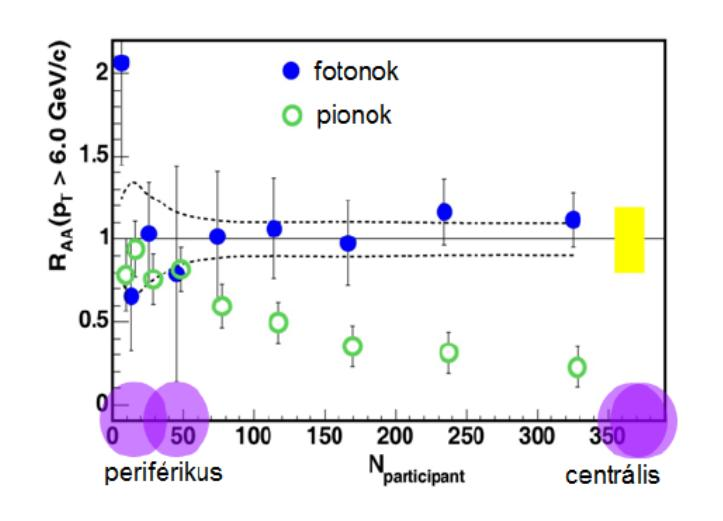
\includegraphics[scale=0.6]{pic/int/p1}
 \caption{Au+Au ütközések esetén a nukleáris módosulási faktor a nukleonszám függvényében pionokra és fotonokra. Az ábrán látható, hogy nagy centralitás esetén kevesebb nagyenergiás piont észlelünk mint p+p ütközések alapján várnánk, továbbá az erős kölcsönhatásban nem 
  fotonok száma a várttal egyezik. Ez utal az erősen kölcsönható közeg jelenlétére. Forrás: ~\cite{CsanadHabil}}
\label{fig:mmf}
\end{figure}
\end{center}

\subsection{Kvark-gluon plazma}

A RHIC gyorsítóban Au+Au ütközések során nagy nagy centralitásnál mérések során kevesebb nagyenergiás részecskét mértek a p+p ütközések alapján vártnál (\ref{fig:mmf} ábra), a jet-párok egyik tagja nem jelent meg. Azonban ezen tapasztalatoknak több kiváltó oka is lehet, a kérdés eldöntésére további kísérleteket végeztek. Az egyik volt a deutérium-arany ütközések elvégzése, azonban itt semmilyen centralitásnál nem volt jet-elnyomás. Ennek magyarázata, hogy ütközések esetén erősen kölcsönható közeg jöhet létre amely a jet-pár egyik tagját elnyeli (amely nagyobb utat tesz meg benne), azonban deutérium-arany ütközések során a létrejövő közeg mérete túl kicsi, hogy elnyelje azt.

Ezen közeg létrejöttét elméletileg a QCD magyarázza meg. Az elmélet szerint nagyon nagy energián megjelennek kvark szabadsági fokok, azaz a kvarkok hadronba zártsága megszűnik. A létrejövő közeg az erősen kölcsönható kvark-gluon plazma nevet viseli (sQGP). Ezen közegben nagyok a hatáskeresztmetszetek, ezért kicsi a szabad úthossz és gyors a termalizáció, ezért van értelme lokális egyensúlyról beszélni, így alkalmazhatóak rá a statisztikus fizika fogalmai (pl. hőmérséklet). Az ősrobbanást követő egy milliomod másodpercben az univerzumot is a kvark-gluon plazma alkotta ~\cite{SWeinberg}.

Az új közeg felfedezése után a RHIC gyorsítóban ezen közeg tulajdonságainak megismerését célzó kísérletek kezdődtek. Ezen kísérletek során kiderült, hogy a kvark-gluon plazma az eddig látott legtökéletesebb (viszkozitás mentes) folyadékként viselkedik, amely meglepő volt hisz nagyon kis viszkozitással rendelkező folyadékokat eddig nagyon alacsony hőmérsékleten tudtak csak előállítani. A kvarkfolyadék viszkozitására a gravitációs- és kvantumtérelméletek analógiájából (AdS/CFT) származik egy alsó becslés, eszerint a viszkozitás nem lehet kisebb mint $\hbar/4\pi$.

\begin{center}
\begin{figure}[H]
\centering
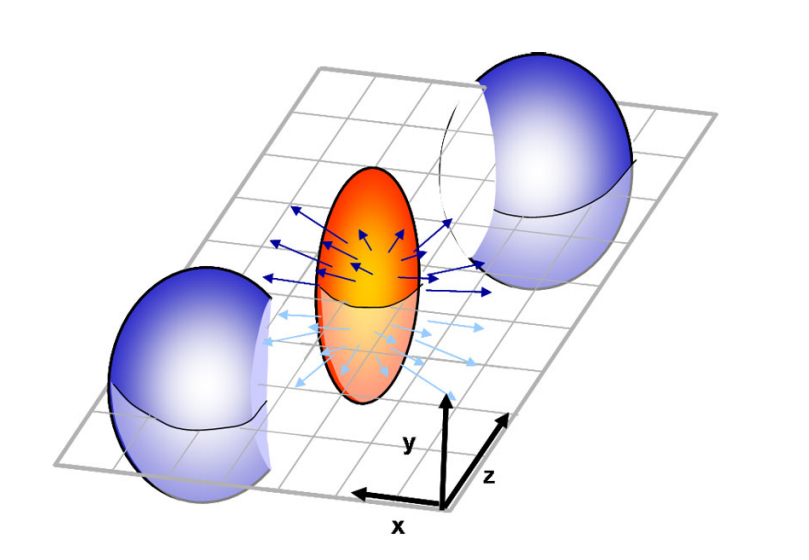
\includegraphics[scale=0.6]{pic/int/p2}
\caption{Két gömb ütközéseként létrejövő speciális ellipszoidális szimmetriával rendelkező kezdeti eloszlás kialakulása. Forrás: ~\cite{CsanadHabil}
}
\label{fig:ellip}
\end{figure}
\end{center}



Ultrarelativisztikus sebességre felgyorsított atommagok ütközése két Lorentz-kontrahált korong ütközéseként fogható fel, laborrendszerből nézve. Amint \aref{fig:ellip} ábra is szemlélteti, ez a létrejövő kvarkanyagban speciális kezdeti eloszlást eredményez, egy $\cos(2\varphi)$-szerinti aszimmetriát az eloszlásban, amely a tengelyszimmetriától való elliptikus eltérést jelenti.
A nyalábirányra merőlegesen bevezetjük a transzverz-síkot, ebben a síkban az kvarkanyag kezdeti eloszlását Fourier-sorba fejtjük a következőképpen:
\begin{large}
\begin{equation}
A(\varphi)= a_0+\sum_{n=1}^{\infty}\Big[a_n \cos(n\varphi)+b_n \sin(n\varphi)\Big]
\label{eq:e2}
\end{equation}
\end{large}
Ezen sorfejtés alapján látható, hogy az $a_2$ jellemzi az előbb említett aszimmetriát, amennyiben tökéletesen gömbszimmetrikusak lennének az atommagok és a keletkező ellipszis egyik nagytengelyén vennénk föl a a koordináta-rendszer x-tengelyét csupán ez a tag jelenne meg. Azonban mivel az atommagok véges nukleonszámmal rendelkeznek, melyeknek van valamilyen eloszlása a magon belül, a gömbszimmetria csupán első közelítésként fogható fel.

Az ütközés után létrejövő kvarkanyag robbanásszerűen tágul egész addig amíg a hőmérséklet le nem csökken egy bizonyos értékre, ekkor megszűnik ez a fázis és a kvarkokból hadronok keletkeznek amelyeket mérni is tudunk. Mivel a kvarkanyag folyadékszerűen viselkedik a kezdeti aszimmetriák nem tűnnek el, a kifagyás pillanatába is jelen vannak, ezért azok a keletkező hadronok eloszlásában is megjelennek. Az aszimmetriákat jellemző paramétereket az impulzustérben szokás definiálni. A részecskék eloszlását transzverz-síkban a $N(p_t, \varphi)$ függvénnyel jellemezzük, amely megmondja, hogy $[\varphi, \varphi+d\varphi]$ irányban $[p_t, p_t+dp_t]$ impulzus-tartományban mennyi részecske található. A függvény szögfüggését leválasztva, azt Fourier-sorba fejtve és 1-re normálva a következő alakban írhatjuk:
 \begin{large}
\begin{equation}
N(p_t, \varphi)= N(p_t)\bigg(1+\sum_{n=1}^{\infty}\Big[v_n \cos(n\varphi)+w_n \sin(n\varphi)\Big]\bigg)
\label{eq:e3}
\end{equation}
\end{large}
A Fourier-sor első komponensei játszanak fontosabb szerepet. Ezek közül is a $v_2$ együttható a leglényegesebb, mert ez a paraméter hordozza az ellipszoidális aszimmetriát, ezt az elliptikus folyás paraméterének nevezzük. Ezen aszimmetria a kifagyott hadronok és fotonok eloszlásában ~\cite{Adare:2011zr} is megjelenik, ezért a folyadékkép helyességét bizonyítja a kvark-gluon plazma esetén.
A Fourier-sor szinuszos részét nem szoktuk külön kezelni, mivel a mérések során a reakciósíkhoz képesti szög szerinti sort veszünk ($\sum v_n \cos[n(\varphi-\psi_n)])$, így a fenti szinuszos és koszinuszos tagok összevonva jelennek meg. Más mérési módszer esetén ugyan megjelenhetnek külön is a szinuszos tagok, de ekkor is szimmetria okokból ezen tagok eltűnnek.


\subsection{A PHENIX kísérlet}

A PHENIX (Pioneering
High Energy Nuclear Interaction eXperiment) kísérlet az Amerikai Egyesült Államok  Brookhaveni Nemzeti Laboratóriumában működő Relativisztikus nehézion-ütköztető (RHIC) egyik detektorrendszere, amelynek adatain 14 ország több száz kutatója dolgozik (PHENIX kollaboráció). A relativisztikus nehézion-ütköztető két, egyenként $3.8$ km kerületű gyorsítógyűrűből áll, amelyek összesen 6 különböző pontban metszik egymást. A metszéspontokba épültek a különböző detektorrendszerek, amelyek közül ma már csak a két legnagyobb, a PHENIX és a STAR rendszerek aktívak.

A PHENIX kísérlet detektorait ~\cite{Adcox:2003zm}, amelyet ~\aref{fig:phenix} ábra szemlélteti, két csoportba oszthatjuk: események globális tulajdonságait meghatározó, illetve az eseményekből kirepülő részecskék észlelését és tulajdonságait mérő detektorok.

\begin{figure}[H]
\centering
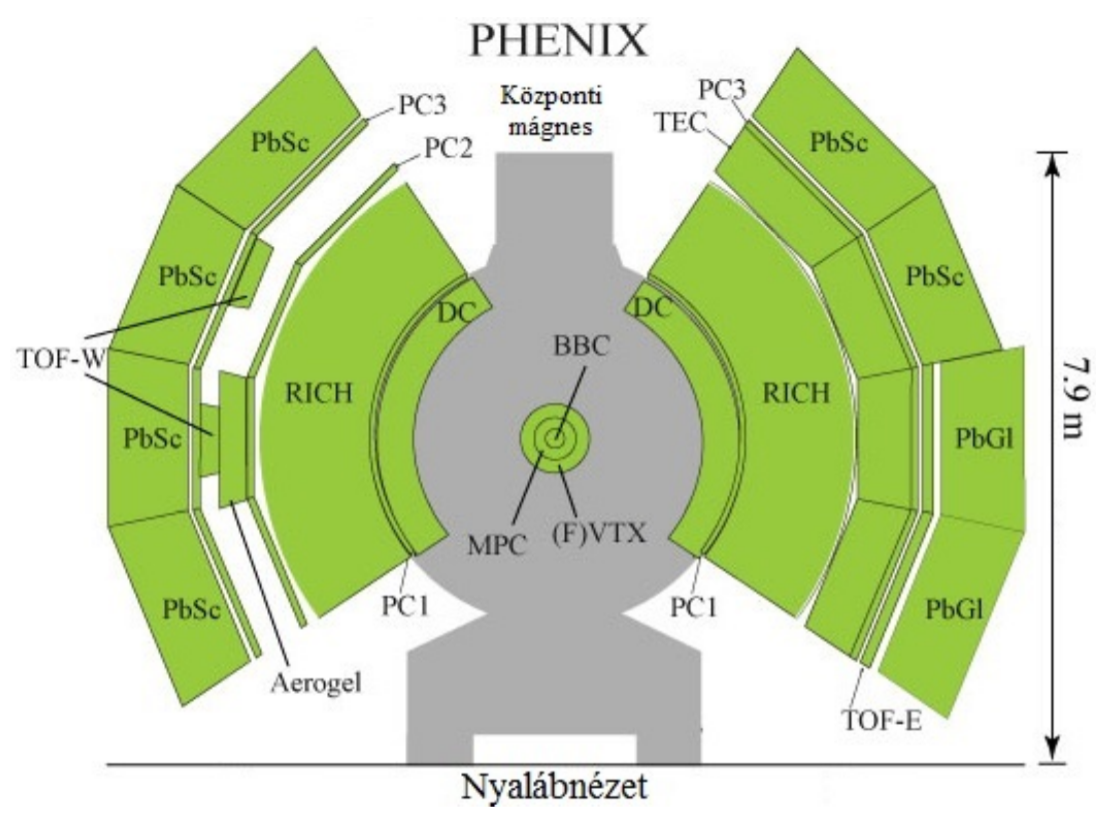
\includegraphics[scale=0.32]{pic/int/phenix1}
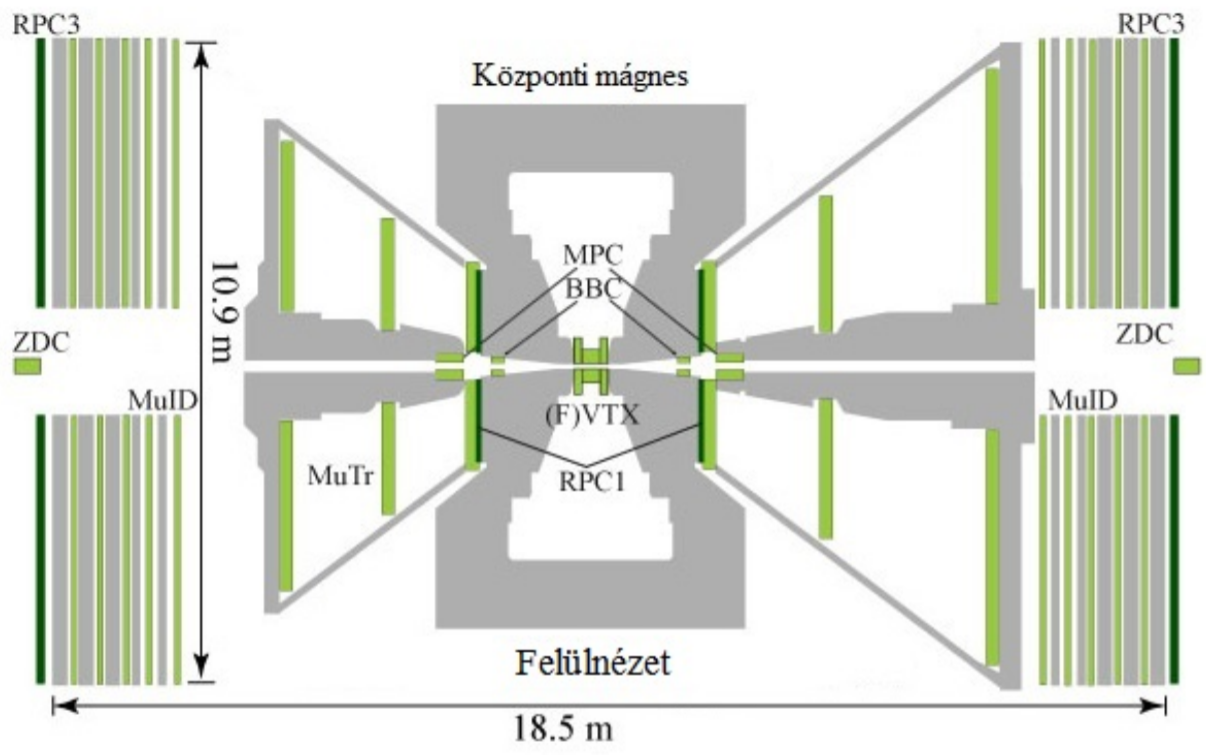
\includegraphics[scale=0.32]{pic/int/phenix2}
\caption{A PHENIX detektorrendszer. A baloldali ábra mutatja a detektorrendszer nyalábirányra merőleges metszetét, a jobboldali pedig nyalábiránnyal párhuzamosat.}
\label{fig:phenix}
\end{figure}

\subsubsection{Eseményjellemző detektorok}\label{sec:phenix1}

Az eseményjellemző detektorok meghatározzák egyrészt, hogy történt-e ütközés (jel a többi detektor számára, hogy mérni kell), másrészt az esemény fontos jellemzőit (ütközés pontos helye, geometriai elrendezése). Ilyen detektorok a Zero Degree Calorimeter (ZDC) és a Beam Beam Counter (BBC), melyek közül az analízis során a BBC detektort használtuk.

A BBC detektor két karból áll, melyek nyalábirányban helyezkednek el egymástól $288$ cm távolságra, mint ~\aref{fig:phenix} jobb oldali ábrán látható. A karokban leadott töltésből meghatározható az esemény centralitása, azaz, hogy a két ütköző atommag mennyire ``középen'' találta el egymást. A két detektor a beérkezési időt is méri, amelynek különbségéből meghatározható az ütközés nyalábiránnyal párhuzamosan vett helye (z-vertex, koordináta-rendszer z tengelyét nyalábiránnyal párhuzamosan vesszük fel). A detektor időfelbontása $40$ ps, amely centrális ütközés esetén $0.5$ cm z-vertex felbontást eredményez.
 
\subsubsection{Részecskeazonosító detektorok}\label{sec:phenix2}

A részecskék azonosítása a részecskék impulzusának és sebességének meghatározásával történik. A sebesség mérése érdekében el kell végezni a részecskék pályájának rekonstrukcióját, amely, az úgynevezett nyomkövető detektorok: a Drift Chamber (DC) és az első Pad Chamber (PC1) segítségével történik (mindkettő sokszálas proporcionális kamra). 

A DC detektorok a nyalábtól $2.02$ és $2.46$ méter távolságra helyezkednek el, és z irányba $180$ cm, transzverz irányba pedig $180^{\circ}$ tartományt fednek le. Ezek a detektorok transzverzális irányba ($\varphi$ szög) mérik a részecskék pályáját $1$ mrad szögfelbontással. A nyalábiránnyal párhuzamos mágneses tér hatására a részecskék pályája elgörbül, így DC detektor által mért görbületi sugárból a részecske transzverz impulzusa meghatározható.

A PC1 detektorok közvetlenül a DC detektorok mögött helyezkednek el, és mind a nyaláb mind transzverz irányban mérik a részecske pályáját ($z$ és $\varphi$). A PC1 detektor által mért $z$ koordinátából és a BBC detektor által meghatározott z-vertex pozícióból meghatározható a részecskék nyalábirányú impulzusa.

A részecskék impulzusa és pályája mellett meg kell határozni a repülési időt, amelyet az  ólom-szcintillátor elektromágneses kaloriméterek (PbSc) illetve repülésidő detektorok (TOF-E, TOF-W) segítségével tehetünk meg. Az elektromágneses kaloriméterek a detektorrendszer legszélén helyezkednek el, mivel ezek a berepülő részecskéket teljes energiájuk elnyerésével észlelik. A PbSc kaloriméterek segítségével pionok esetén körülbelül $400$ ps időfelbontás érhető el. A TOF-E repülésidő detektor a keleti szárnyban helyezkedik el közvetlenül a PbSc detektor előtt, azonban nem fedi le a teljes keleti oldalt. Ez a detektor fotoelektron-sokszorozókkal ellátott műanyag szcintillátorból áll, segítségével $140$ ps pontossággal mérhető a repülésidő. A TOF-W detektor a nyugati szárnyban, szintén a PbSc detektorok előtt helyezkedik el, valamint két különálló panelből áll. Ezen panelek sokréses ellenállás-kamra (resistive plate chamber) detektorok, amelyek $90$ ps felbontással képesek repülésidőt mérni.


A DC/PC1 detektorok által rekonstruált pályából meghatározható a részecske által megtett út ($L$), továbbá a TOF/PbSc és BBC detektorok segítségével mérhető a repülési idő ($t$), melyekből megkapjuk a részecskék sebességét. Továbbá a DC/PC1 detektorok a részecske impulzusát is meghatározza, így minden szükséges mennyiséget ismerünk a részecske azonosításához. Ezen mennyiségekkel az azonosításhoz szükséges tömegnégyzet a következőképpen alakul:

\begin{equation}
m^2=\frac{p^2}{c^2}\Bigg[\bigg(\frac{ct}{L}\bigg)^2-1\Bigg]
\label{eq:m2}
\end{equation}

\section{Bose-Einstein korrelációk}

Bose-Einstein korrelációk vizsgálatának megalapozói Robert Hanbury Brown és Richard Q. Twiss volt, ők 1956-ban publikált cikkükben ~\cite{HanburyBrown:1956bqd} vezették be a módszert, azonban munkájuk vegyes fogadtatásban részesült a tudományos közösség részéről. A módszer segítségével képesek voltak meghatározni a Sirius csillag átmérőjét a fotonok közötti korrelációk méréséből. Mérési elrendezésük két változtatható távolságra levő foton detektorból állt (ezek egy-egy fókuszáló tányér és fotoelektron-sokszorozóból álltak). A két detektor segítségével mérték a Sirius csillagból jövő fotonok közti korrelációt, különböző detektortávolságokon. Az így kapott pontokra elméleti megfontolásokból kapott korrelációs függvényt illesztettek, amely segítségével meghatározták a csillag átmérőjét. A két tudós tiszteletére a bozonok közti intenzitás korrelációt szokás Hanbury Brown és Twiss effektusnak nevezni (vagy röviden HBT effektus), az ilyen jellegű vizsgálódásokat pedig HBT analízisnek.

A HBT effektus részecskefizikai alkalmazásában jelentős szerepet játszott G. Goldhaber, S. Goldhaber, W.Y. Lee és A. Pais kutatása, akik proton-antiproton $1.05\;\mathrm{GeV/c}$ tömegközépponti energián történő ütköztetésekben keletkező pionokat vizsgáltak. Mérésük során azonos pionok között nem várt korrelációt tapasztaltak, melynek vizsgálatával felfedezték a $\rho^0$ rezonanciát, amely $4.5\cdot 10^{-24}$ másodperc alatt elbomlik két pionra ($\rho^0\rightarrow \pi^+\pi^-$), eredményüket 1960-ban publikálták ~\cite{Goldhaber:1960sf}. Később kiderült, hogy az általuk tapasztalt korrelációnak az oka, hogy a fotonokhoz hasonlóan a pionok is bozonok. Goldhaber és társai kutatása nyomán a részecskefizikában is beindult a HBT effektus vizsgálata. Későbbiekben kiderült, hogy az asztrofizikához hasonlóan ezek a korrelációk itt is információt hordoznak a forrás geometriájáról ~\cite{Padula:2004ba, CsanadHabil}. 


\subsection{Definíció}

Általánosan $n$ részecske közti korrelációs függvény a következőképpen definiálható ~\cite{Alt:1999cs, Csorgo:1999sj}:
\begin{equation}
C_n(p_1, p_2, \dots, p_n)=\frac{ N_n(p_1, p_2, \dots, p_n)  }{ N_1(p_1)N_1(p_2)\dots N_1(p_n)},
\label{eq:Cn}
\end{equation}
ahol $p_i=(p_i^0, \bm{p_i})$ 4-es impulzusmomentum, $ N_n(p_1, p_2, \dots, p_n)$ az $n$ részecske invariáns momentum eloszlás. A korrelációs függvény szemléletesen azt mondja meg, hogy milyen valószínűséggel keletkezik egy részecske n-es $p_1, p_2, \dots, p_n$ 4-es momentumokkal.

Az $n$ részecske invariáns impulzusmomentum eloszlás meghatározható a következő módon:
\begin{equation}
N_n(p_1, p_2, \dots, p_n) = \int \prod_{i=1}^{n}\mathcal{S}(p_i, x_i)\abs{\Psi_{p_1, {p_2}, \dots, {p_n}}({x_1}, {x_2}, \dots, {x_n})}^2\prod_{i=1}^{n}d^4 x_i,
\label{eq:Nn}
\end{equation}
ahol a $\Psi_{p_1, {p_2}, \dots, {p_n}}({x_1}, {x_2}, \dots, {x_n})$ az $n$ részecske hullámfüggvény, az $\mathcal{S}({p_i}, {x_i})$ pedig az úgynevezett forrásfüggvény, amely megadja annak a valószínűségét, hogy ${x_i}$ helyen keletkezik egy részecske ${p_i}$ impulzussal.

Az $n$ részecske hullámfüggvény meghatározásához nemrelativisztikus közelítést használunk HBT effektus vizsgálata során, így a függvényt a Schrödinger egyenlet megoldásából kapjuk (ügyelve, arra hogy mivel bozonjaink vannak, két részecske felcserélésére szimmetrikus legyen a hullámfüggvény):
\begin{equation}
i\hbar\frac{\partial \Psi(\bm{x_1},\dots, \bm{x_n},t )}{\partial t} = \Bigg[\sum_{i=1}^{n}\bigg(-\frac{\hbar^2}{2m_i}\Delta_i + V_i(\bm{x_i})\bigg) + \frac{1}{2}\sum_{i\neq j} V_{ij}(\bm{x_i},\bm{x_j})\Bigg]\Psi(\bm{x_1},\dots, \bm{x_n} ,t)
\label{eq:Sch0}
\end{equation}

A HBT effektus vizsgálatánál a különböző számítások könnyítése érdekében elhanyagoljuk az erős kölcsönhatást, amely tapasztalatok szerint pionok esetén megtehető, de már protonok esetén nem ~\cite{Pratt:1990zq}. Továbbá csak a párok közti Coulomb-kölcsönhatást vesszük figyelembe, elhanyagolva többi hadron által okozott töltésfelhőt. Így ~\aref{eq:Sch0} egyenlet a következő, egyszerűbb alakra egyszerűsödik:
\begin{equation}
i\hbar\frac{\partial \Psi(\bm{x_1},\dots, \bm{x_n},t )}{\partial t} = \Bigg[-\sum_{i=1}^{n}\frac{\hbar^2}{2m_i}\Delta_i + \frac{1}{2}\sum_{i\neq j} V_\mathcal{C}(\bm{x_i},\bm{x_j})\Bigg]\Psi(\bm{x_1},\dots, \bm{x_n} ,t)
\label{eq:Sch}
\end{equation}

Mivel energia saját állapotokkal dolgozunk, ezért  ~\aref{eq:Sch} egyenletet megoldó hullámfüggvény felírható:
\begin{equation}
\Psi_{p_1, {p_2}, \dots, {p_n}}(\bm{x_1},\dots, \bm{x_n},t )  
= \Psi_{\bm{p_1}, \bm{p_2}, \dots, \bm{p_n}}(\bm{x_1}, \bm{x_2}, \dots, \bm{x_n})\prod_{i=1}^ne^{-\frac{i}{\hbar}cp_i^0t},
\end{equation}
ahol $\Psi_{\bm{p_1}, \bm{p_2}, \dots, \bm{p_n}}(\bm{x_1}, \bm{x_2}, \dots, \bm{x_n})$ az időfüggetlen Schrödinger egyenlet megoldása:

\begin{equation}
\Bigg[-\sum_{i=1}^{n}\frac{\hbar^2}{2m_i}\Delta_i + \frac{1}{2}\sum_{i\neq j} V_\mathcal{C}(\bm{x_i},\bm{x_j})  
 - c\sum_{i=1}^n p_i^0
 \Bigg]\Psi_{\bm{p_1}, \bm{p_2}, \dots, \bm{p_n}}(\bm{x_1}, \bm{x_2}, \dots, \bm{x_n}) = 0
\end{equation}

Továbbá könnyedén belátható, hogy ~\aref{eq:Nn} egyenletben szereplő hullámfüggvény abszolút értéke szimmetrizációt elvégezve a következő lesz  (nemrelativisztikus közelítésben mondhatjuk, hogy $\bm{x_i} = (t,\bm{x_i})$) :
\begin{equation}
\abs{\Psi_{{p_1},{p_2}, \dots,{p_n}}({x_1}, {x_2}, \dots, {x_n})} = \frac{1}{\sqrt{n}}\abs{\sum_{(\alpha)}\Psi_{\bm{p_1}, \bm{p_2}, \dots, \bm{p_n}}(\bm{x_{\alpha_1}}, \bm{x_{\alpha_2}}, \dots, \bm{x_{\alpha_n}})}
\label{eq:Psin}
\end{equation}
ahol $\sum_{(\alpha)}$ az $(1,2,\dots,n)$ összes permutációjára való összegzés.


\subsection{Két nem kölcsönható részecske korrelációs függvénye}\label{sec:C20}

Két azonos részecske esetén, nem kölcsönható esetben ~\aref{eq:Sch} egyenlet könnyedén megoldható, megoldásai a jól
ismert síkhullámok. A kétrészecskés invariáns impulzuseloszlásban szereplő hullámfüggvény szimmetrizáció
elvégzése után a következő lesz:
\begin{equation}
\Psi_{{p_1}{p_2}({x_1},{x_2})} = \frac{1}{\sqrt{2}}\big({e^{{ip_1x_1}+i{p_2x_2}}+e^{i{p_2x_1}+i{p_1x_2}}}\big)
\end{equation}

Tömegközépponti koordináta rendszerben, azaz a következő változókra való áttérés után (ezen transzformáció esetén az integrálási mérték nem változik, hiszen $d^4x_1d^4x_2=d^4Rd^4r$):
\begin{equation}
{K}=\frac{p_1+p_2}{2},\;\;\;\;{k}=\frac{{p_1-p_2}}{2},\;\;\;\;{r}={x_1-x_2},\;\;\;\;{R}=\frac{{x_1+x_2}}{2}
\label{eq:CMF}
\end{equation}
\noindent
a hullámfüggvény abszolút értéke a következő alakra egyszerűsödik:
\begin{equation}
\abs{\Psi_{{p_1}{p_2}}({r},{R})} = \frac{1}{\sqrt{2}}\abs{e^{i{2KR}}(e^{i{kr}}+e^{-i{kr}})}=\sqrt{2}\abs{\cos{2{kr}}}
\end{equation}

Ebből következőleg a kétrészecske invariáns momentumeloszlásra a következő alak adódik):
\begin{equation}
N_2({p_1},{p_2})=\tilde{\mathcal{S}}(0, {p_1})\tilde{\mathcal{S}}(0, {p_2})+\frac{1}{2}\big(\tilde{\mathcal{S}}(2{k}, {p_1})\tilde{\mathcal{S^*}}(2{k}, {p_2})+\tilde{\mathcal{S^*}}(2{k},{ p_1})\tilde{\mathcal{S}}(2{k}, {p_2})\big),
\end{equation}
\noindent
ahol $\tilde{\mathcal{S}}$ a forrásfüggvény Fourier transzformáltja:
\begin{equation}
\tilde{\mathcal{S}}({q}, {k})=\int d^4x\mathcal{S}(x,k)e^{i{qx}}
\end{equation}

Az egyrészecske invariáns momentumeloszlásra pedig $N_1({p})=\tilde{\mathcal{S}}(0, {p})$ adódik. Ezekből ~\aref{eq:Cn} definíciót használva a kétrészecske korrelációs függvényre kapjuk a következő alakot:

\begin{equation}
C_2({p_1},{p_2}) = 1+ \frac{\tilde{\mathcal{S}}(2{k}, {p_1})\tilde{\mathcal{S^*}}(2{k}, {p_2})+\tilde{\mathcal{S^*}}(2\bm{k},{ p_1})\tilde{\mathcal{S}}(2\bm{k}, {p_2})}{2\tilde{\mathcal{S}}(0, {p_1})\tilde{\mathcal{S}}(0, {p_2})}
\end{equation}

Szokás alkalmazni a ${p_1}\approx {p_2}\approx {K} = p_1+p_2$ közelítést ($q\ll K$), amelyet az indokol, hogy a forrás Fourier transzformáltjának az egyes részecskék momentumától való függése sokkal simább mint a relatív momentumtól való függése ~\cite{Lisa:2005dd}. A kétrészecske korrelációs függvény ekkor: 
\begin{equation}
C_2({k}, {K})=1+\frac{\abs{\tilde{\mathcal{S}}({k},{K})}^2}{\abs{\tilde{\mathcal{S}}(0,{K})}^2}
\label{eq:C02}
\end{equation}

Ez az alak azt a fontos üzenetet hordozza, hogy a kétrészecske korrelációs függvény meghatározásával megkapjuk a forrásfüggvény Fourier transzformáltját. Tehát a korrelációs függvény méréssel a forrás függvényt meg tudjuk határozni. 


A korrelációs függvény a $k,K$ négyes impulzusok helyett hármas momentumokkal is kifejezhető, ugyanis a két négyesmomentum szorzata definíció és az egyes részecskék tömeghéj feltétele ($p_{i\mu}p^{\mu}_i=0$) alapján eltűnik, azaz:
\begin{equation}
0=kK=k_0K_0-\bm{kK}\Rightarrow k_0 = \frac{\bm{kK}}{K_0}
\label{eq:kK}
\end{equation}

A $p_1\approx p_2\approx K$ feltevés alapján a $K$ körülbelül tömeghéjon van, azaz $K_0 = \sqrt{m^2-\bm{K}^2}$, így a korrelációs függvény a $k,K$ négyes-momentumok helyett a $\bm{k},\bm{K}$ hármas-momentumok függvényeként is tekinthető. Ezen közelítés jogosságát ~\cite{Wiedemann:1999qn, Csorgo:1999sj} cikkek részletesen tárgyalják.

\subsection{Forrás függvény}
~\Aref{eq:Nn} egyenletben szereplő $\mathcal{S}({p},{x})$ függvényt nevezzük forrásfüggvénynek, ez megadja annak a valószínűségét, hogy ${x}$ helyen keletkezik egy ${p}$ impulzusú részecske. Az általunk vizsgált energiákon, az ütközés során kvark-gluon plazma keletkezik, amely robbanásszerűen tágul, melynek következtében csökken a hőmérséklete. Ha lokálisan a QGP elér egy bizonyos hőmérsékletet, akkor fázisátmenet történik, kifagynak a kvark szabadsági fokok és hadronok keletkeznek. A forrásfüggvényt épp ezen fázisátmenetek határozzák meg. 

A fázisátmenetet pillanatszerűnek tekinthetjük, mivel ha feltesszük, hogy ez nem teljesül, akkor mondhatjuk, hogy a forrásfüggvény felírható szorzat alakban: $\mathcal{S}({x}) = \mathcal{S}_T(\tau)\mathcal{S}(\bm{x})$. Az időfüggő részre feltehető továbbá (\cite{CsanadHabil}):
\begin{equation}
\mathcal{S}_T(\tau)=\frac{1}{(2\pi \Delta\tau)^\frac{3}{2}}e^{-\frac{(\tau-\tau_0)^2}{2\Delta\tau^2}}
\end{equation}

Térszerű részre kevés megszorítással élve, a kétrészecske korrelációs függvényre a következő alak adódik (\cite{CsanadHabil}):
\begin{equation}
C_2(k)=1+\lambda e^{-k_0\Delta\tau^2-k_{\mathrm{long}}R_{\mathrm{long}}^2-k_{\mathrm{side}}R_{\mathrm{side}}^2-k_{\mathrm{out}}R_{\mathrm{out}}^2},
\end{equation}
ahol az $R_{\mathrm{long}},R_{\mathrm{side}},R_{\mathrm{out}}$ az úgynevezett HBT sugarak. Továbbá adódik a HBT sugarak közti következő összefüggés (\cite{CsanadHabil}):
\begin{equation}
R_{\mathrm{out}}^2-R_{\mathrm{side}}^2\propto \Delta\tau^2
\end{equation}

Kísérleti tapasztalat továbbá, hogy $R_{\mathrm{out}}\approx R_{\mathrm{side}}$, ebből következőleg a $\Delta\tau\approx 0$, tehát, a  forrásfüggvény időfüggő része egy $\tau_0$-ra koncentrált Dirac-delta, azaz a fázisátmenet pillanatszerűen történik ~\cite{Ster:2010ia, Csorgo:1999sj, Csanad:2009wc}.

%~\Aref{eq:Psin} egyenletnél láttuk, hogy az invariáns momentum eloszlásban megjelenő hullámfüggvény időfüggetlen.


A forrásfüggvény alakjára elsődlegesen Gauss eloszlást alkalmaztak ~\cite{Csorgo:2005gd, Lisa:2005dd}, azonban a PHENIX kísérletben $\sqrt{s_{NN}}=200\;\mathrm{GeV}$ tömegközépponti energiájú arany-arany ütközések során bizonyítékot találtak nem gaussi, lassan lecsengő struktúrára ~\cite{Adler:2006as}. Egy magyarázat a lassan lecsengő viselkedésre lehet a Lévy repülés ~\cite{Csanad:2007fr}. A kvark-glon plazmából már kifagyott hadronok gáza tágul, így a rendszer egyre hidegebb, ritkább lesz, a hatáskeresztmetszetek egyre kisebbé válnak, megnövelve az átlagos szabad úthosszat. Ennek következtében egyre hosszabb lépések is megjelennek a hadronok véletlen bolyongás során. Ennek következtében eltávolodás eloszlása lassan lecsengő eloszlás lesz, melynek szórása már nem létezik. Ezen véletlen bolyongó hadronok aztán elbomolhatnak a vizsgált részecskékre, ezért járulékot adnak a forrásfüggvénybe. Ezen hadronok eltávolodása (QGP-ből való kifagyás helyétől), a centrális határeloszlás tétele alapján Lévy eloszláshoz tart, hiszen az összeadott lépések lassan lecsengő eloszlással rendelkező valószínűségi változónak tekinthető.

\subsubsection{Lévy eloszlás}

A forrásfüggvény alakjára munkám során három dimenziós Lévy eloszlást használtam. A Lévy eloszlás három dimenzióban a következő karakterisztikus függvény segítségével adható meg:
\begin{equation}
\Phi(\bm{q}, \alpha, R) = e^{-\abs{\bm{q}R}^\alpha}
\end{equation}
A karakterisztikus függvény Fourier transzformáltját kiszámolva (az integrálás csak numerikusan végezhető el) megkapható a Lévy eloszlás:
\begin{equation}
\mathcal{L}(\bm{r},\alpha,R) = \frac{1}{(2\pi)^3}\int d^3q \Phi(\bm{q}, \alpha, R)e^{i\bm{qr}}= \frac{1}{(2\pi)^3}\int e^{i\bm{qr}}e^{-\abs{\bm{q}R}^\alpha},
 \label{eq:Levyint}
\end{equation}
\noindent
ahol $0< \alpha \leq 2$ és $0<R$ a Lévy eloszlás paraméterei. Speciálisan, $\alpha=2$ esetén a Lévy eloszlás a normális eloszlás lesz:
\begin{equation}
\mathcal{N}(\bm{r},\sigma) = \mathcal{L}\bigg(\bm{r}, \frac{\sigma}{\sqrt{2}}\bigg) = \mathcal{L}\big(\bm{r}, 2^{-\frac{1}{\alpha}}\sigma\big)
\end{equation}

Mivel Lévy eloszlást használunk a forrás modellezésére, ezért a Lévy paraméterek a forrásról hordoznak információt, és magára a forrásra jellemzőek. Egy $\alpha, R$ paraméterű forrás esetén, a forrásfüggvényre a következő alakot használjuk:
\begin{equation}
\mathcal{S}(p,x; \alpha, R) =\mathcal{L}\big(\bm{x}, \alpha, 2^{-\frac{1}{\alpha}}R\big)
\end{equation}

A Lévy eloszlás skálaparamétertől való függésére ($R$ paraméter) teljesül a következő összefüggés:
\begin{equation}
\mathcal{L}(\bm{r}, \alpha, R) = \mathcal{L}\bigg(\frac{\bm{r}}{R}, \alpha, 1\bigg)R^{-3}\equiv \mathcal{L}\bigg(\frac{\bm{r}}{R}, \alpha\bigg)R^{-3}
\label{eq:LevyintR}
\end{equation}

Továbbá az eloszlás nem függ az $\bm{r}$ irányától, csak a nagyságától (belátható változócsere segítségével $\bm{q'}=\bm{Aq}$: $\abs{\bm{q}}=\abs{\bm{q'}}\bm{qr}=\abs{\bm{q}}\abs{\bm{r}}$, ekkor $d^3 q=d^3 q'$):
\begin{equation}
\mathcal{L}(\bm{r}, \alpha, R)=\mathcal{L}(\abs{\bm{r}}, \alpha, R)
\label{eq:LevyintO}
\end{equation}

Az egydimenziós Lévy eloszlás aszimptotikus viselkedéséből  ~\cite{LevyEff} kiindulva könnyedén meghatározható a háromdimenziós eloszlás viselkedése is. Nagy $r$ paraméter esetén, a Lévy eloszlás a következő sor segítségével kapható meg ($r>>1$):

\begin{equation}
\mathcal{L}(r,\alpha) \approx \frac{\alpha}{2\pi^2}\sum_{k=1}^{N}(-1)^{k+1}\frac{\Gamma(\alpha k)}{\Gamma(k)} \sin{\bigg(\frac{\pi\alpha k}{2}\bigg)}\frac{\alpha k+1}{r^{\alpha k+3}},
\end{equation}
ahol $\Gamma(x)$ a Gamma függvény:
\begin{equation}
 \Gamma (z)=\int _{0}^{\infty }x^{z-1}e^{-x}\,dx
 \label{eq:gamma}
\end{equation}

A kis $r$ viselkedés hasonló módon egy sor segítségével kapható ($r<<1$):
\begin{equation}
\mathcal{L}(r,\alpha) \approx -\frac{1}{2\pi^2\alpha}\sum_{k=0}^n\frac{\Gamma\big(\frac{k+3}{\alpha}\big)}{\Gamma(k+3)}\sin{\bigg(\frac{\pi(k+3)}{2}\bigg)}(k+2)(k+1)x^k
\end{equation} 

A Lévy eloszlás meghatározása során kis és nagy értékekre ezen aszimptotikus sorokat alkalmaztam, a köztes tartományban pedig 15 pontú adaptív Gauss Kronrod integrálási módszert alkalmaztam (részletek \aref{sec:GK} fejezetben), melyet GPU-ra párhuzamosítva CUDA-ban (részletek \aref{sec:CUDA} fejezetben), továbbá klasztere párhuzamosítva MapReduce programozási modellben implementáltam (részletek \aref{sec:MapReduce} fejezetben). Az integrálást sok paraméterre elvégeztem (felbontást úgy állítottam be, hogy két pont között lineáris interpoláció hibája a megengedett hiba alatt legyen), eredményekből egy Lévy táblázat készült, amelyhez egy könnyen használható olvasó interfész tartozik. Néhány $\alpha$ és $R$ paraméter esetén az eloszlást \aref{fig:Levy} ábrák szemléltetik.

\begin{figure}[H]
\centering
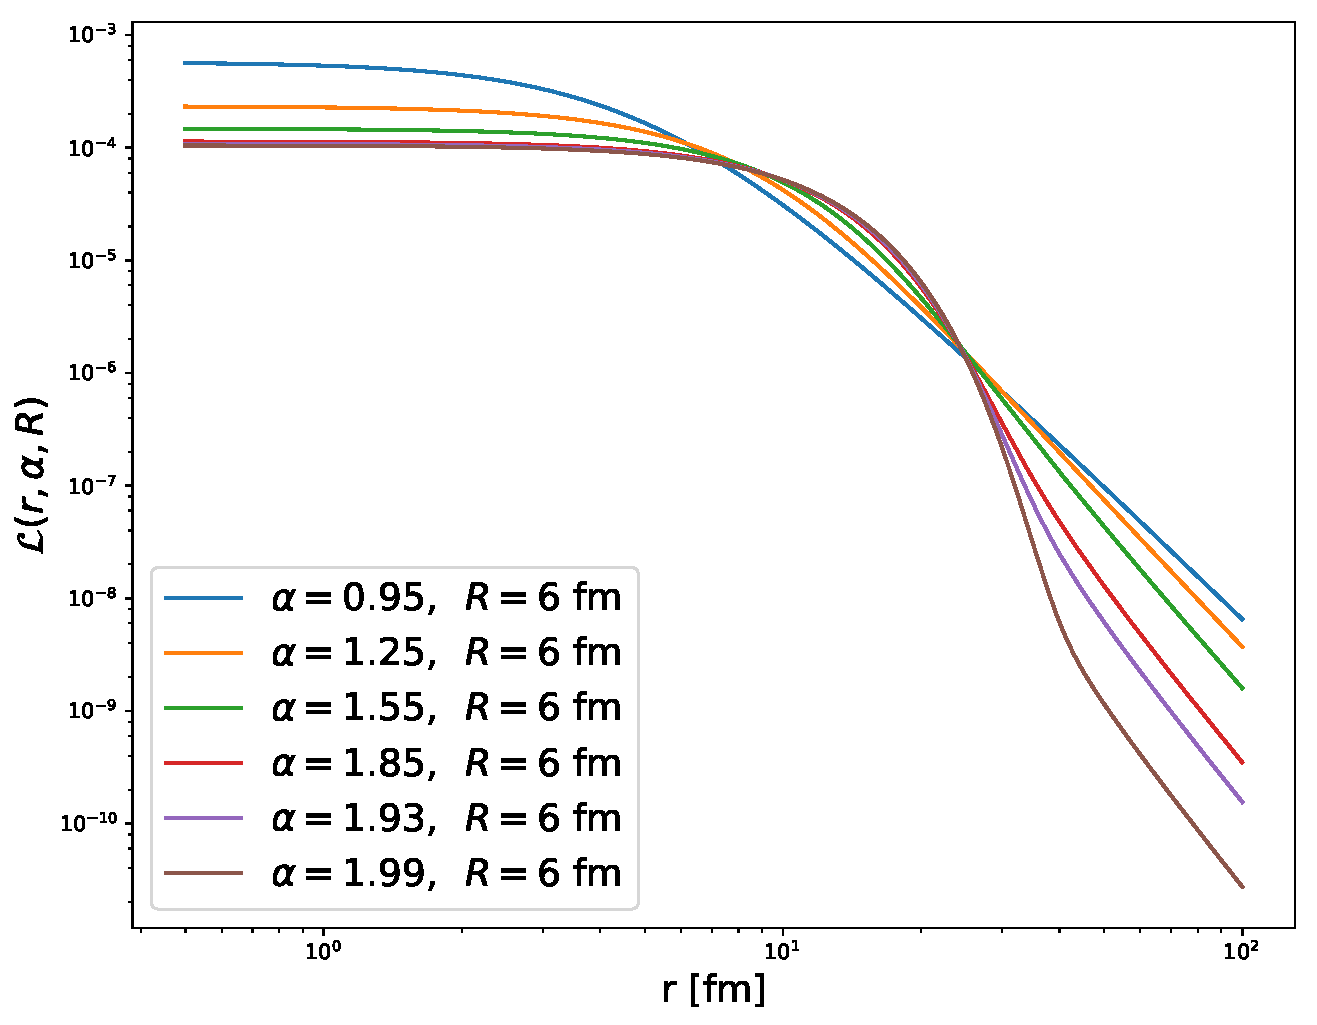
\includegraphics[scale=0.35]{pic/BEintro/Levy_alpha.pdf}
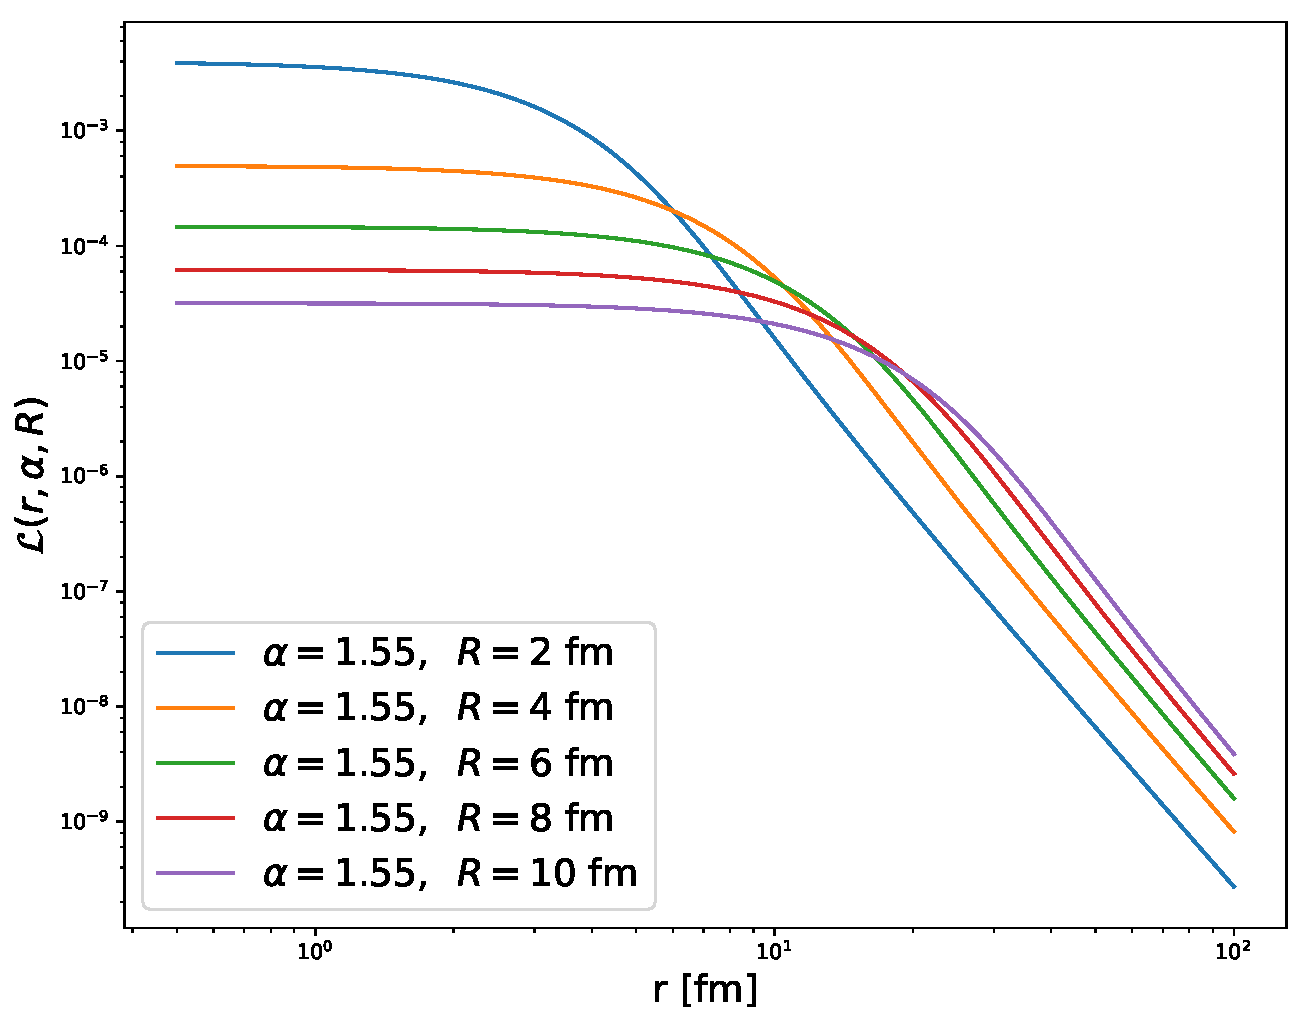
\includegraphics[scale=0.35]{pic/BEintro/Levy_R.pdf}
\caption{Háromdimenziós Lévy eloszlás sugárfüggése különböző $\alpha$ és $R$ paraméterek esetén.}
\label{fig:Levy}
\end{figure}

\subsection{A mag-glória modell}
A HBT effektus vizsgálata során nehéz ionokat ütköztetünk nagy energián. Az ütközés során létrejövő kvark-gluon plazma robbanásszerűen tágul (ezen tágulás leírására hidrodinamika alkalmazható), elérve egy kritikus hőmérsékletet fázisátmenet történik, hadronok fagynak ki pillanatszerűen. A hadronok közül munkánbana  töltött pionok közti korrelációt vizsgáltam, mivel ezen részecskékből keletkezik a legtöbb az ütközések során. A kirepülő pionokat az ütközési centrum köré épített detektorrendszerrel detektáljuk. Azonban pionok nem csak a forró kvarkanyag kifagyása során  keletkeznek, hanem később, instabil részecskék (pl. $\eta,\eta',\omega$) bomlásából is ~\cite{Bolz:1992hc}. Ezen jelenség leírására szolgál a mag-glória (core-halo) modell ~\cite{Csorgo:1994in,Csorgo:1999sj}, melynek szemléltetése ~\aref{fig:ch1} ábrán látható. A mag mérete $10$ femtométer alatti, míg a glória mérete több száz, vagy akár több ezer femtométer is lehet, mivel egyes hosszú élettartamú instabil részecskék ilyen távolságokra jutnak el mielőtt elbomlanának pionokra.
\begin{figure}[H]
\centering
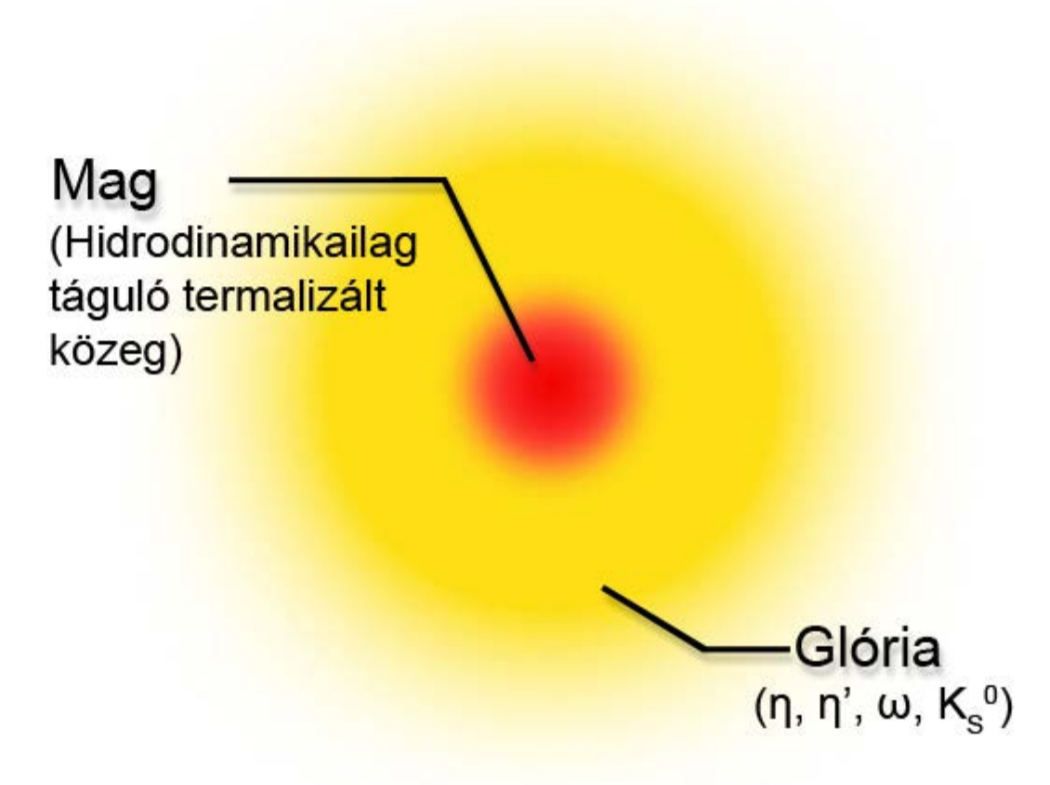
\includegraphics[scale=0.5]{pic/BEintro/CH1}
\caption{Mag-glória modell szemléltetése. Forrás \cite{Kofarago}}
\label{fig:ch1}
\end{figure}

Mivel ~\aref{eq:C02} összefüggés alapján a korrelációs függvény a forrás Fourier transzformáltjával áll kapcsolatban, továbbá a glóriában a pionok nagy $x$ távolságokon keletkeznek, ezért a glória  kis relatív impulzusú tartományban ad járulékot a korrelációs függvényhez. Ugyanakkor a detektor impulzusfelbontása véges, ezért az egymáshoz nagyon közeli impulzussal rendelkező részecskék nem megkülönböztethetőek, azaz bizonyos relatív impulzus alatti tartományban (felbonthatatlan régió) nem tudjuk megmérni a korrelációs függvényt. Ezt az effektust szemlélteti ~\aref{fig:ch2} ábra.

A mag-glória modellben feltételezünk egy magot valamint egy glóriát leíró forrásfüggvény lététezését. A teljes rendszert leíró forrásfüggvény pedig ezen kettő összege:
\begin{equation}
\mathcal{S}(x,p)=\mathcal{S}_M(x,p)+ \mathcal{S}_G(x,p)\Longrightarrow \mathcal{\tilde{S}}(k, K) = \mathcal{\tilde{S}}_M(k,K)+\mathcal{\tilde{S}}_G(k,k)
\end{equation}

Mivel a Fourier transzformált a nulla helyen megegyezik a függvény integráljával, továbbá a forrásfüggvény integrálja a keletkezett részecskék számát adja meg, ezért ha a magban keletkező részecskék száma $N_M$, a glóriában $N_G$, akkor:
\begin{equation}
\mathcal{\tilde{S}}_M(0,K) = N_M,\;\;\;\;\; 
\mathcal{\tilde{S}}_G(0,K) = N_G,\;\;\;\;\;
\mathcal{\tilde{S}}(0,K) = N_M+N_G
\end{equation}

A nagy (legalább $50$ fm) szélességű $\mathcal{S}_G$ keskeny $\mathcal{\tilde{S}}_G$ Fourier transzformáltat eredményez, melynek  szélessége maximálisan $4$ MeV. Ez a maximális szélesség a detektor véges felbontóképességéből adódó felbonthatatlan régióba esik tipikusan, ezért az mondható, hogy: $\mathcal{\tilde{S}}_G\approx 0$, azaz $\mathcal{\tilde{S}}=\mathcal{\tilde{S}}_M$. Ebből a kétrészecske korrelációs függvényre adódik:
\begin{equation}
C_2({k}, {K})=1+\frac{\abs{\tilde{\mathcal{S}}({k},{K})}^2}{\abs{\tilde{\mathcal{S}}(0,{K})}^2} =
1+\frac{\abs{\tilde{\mathcal{S}}_M({k},{K})}^2}{\Big(N_M+N_G\Big)^2}
 =
  1+\lambda_2\frac{\abs{\tilde{\mathcal{S}}_M({k},{K})}^2}{\abs{\tilde{\mathcal{S}}_M(0,{K})}^2},
 \label{eq:CHC2}
\end{equation}
ahol bevezettem a:
\begin{equation}
\lambda_2=\frac{N_M^2}{\Big(N_M+N_G\Big)^2} \equiv f_C^2
\label{eq:CHlambda2}
\end{equation}
jelölést. Az összefüggésben bevezettem egy új mennyiséget, a mag arányt arányát, amely megmondja, hogy az összes észlelt részecske, hányad része származik a magból:
\begin{equation}
f_C=\frac{N_M}{N_M+N_G}
\label{eq:fC}
\end{equation}

Tehát amíg ~\aref{eq:C02} egyenletben a $k\rightarrow 0$ esetben a korrelációs függvény $C_2(k,K)\rightarrow 2$, addig mag-glória modellben, a $2$ helyett a $1+\lambda_2$-höz tart a korrelációs függvény.

\begin{figure}[H]
\centering
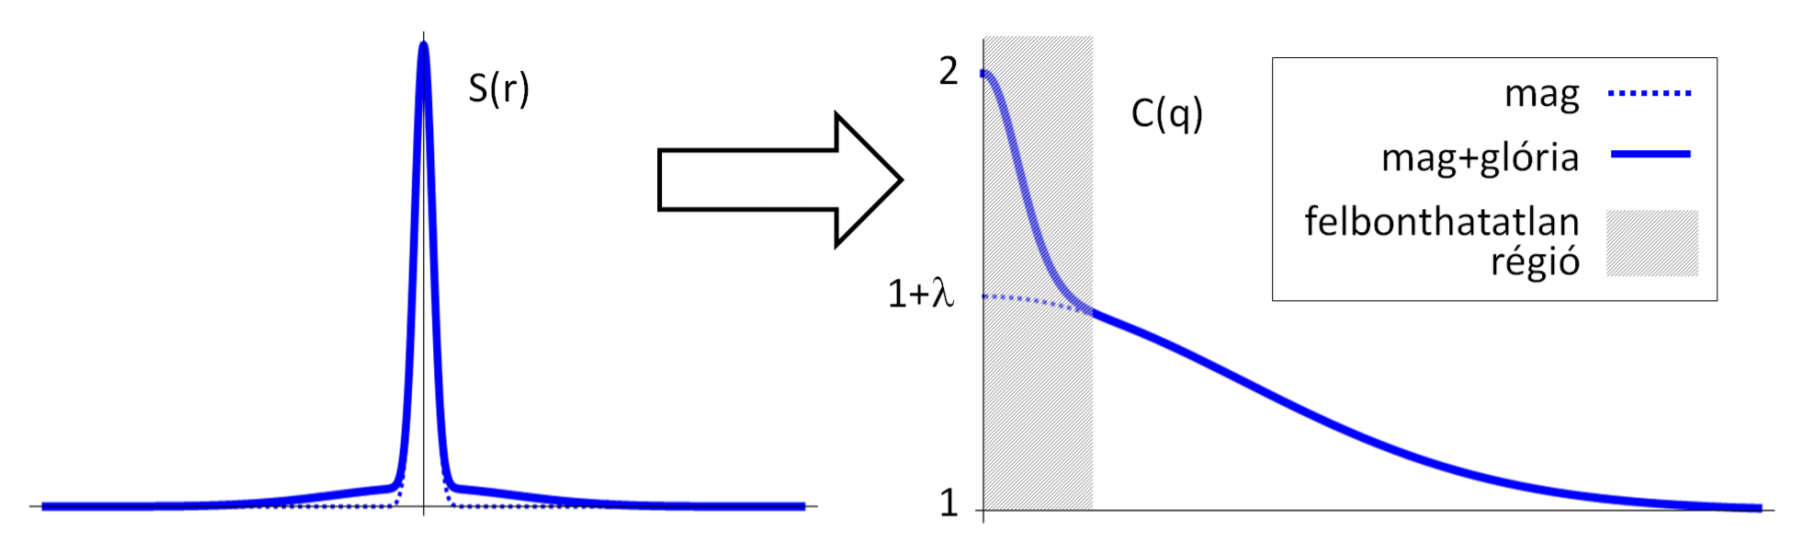
\includegraphics[scale=0.4]{pic/BEintro/CH2}
\caption{Keskeny magból és széles glóriából álló forráshoz tartozó korrelációs függvény. A glória keskeny csúcsot eredményez a korrelációs függvényben, amely a detektor véges felbontásának következtében nem látható. Forrás: ~\cite{CsanadHabil}}
\label{fig:ch2}
\end{figure}


\subsection{A korreláció erőssége}
A mag-glória modellnél láttuk, hogy a kétrészecske korrelációs függvény kis relatív impulzusokra tart ~\aref{eq:CHlambda2} egyenlet által definiált $\lambda_2$ paraméter által meghatározott $1+\lambda_2$ értékhez. Ezt a paramétert szokás kétrészecske korrelációs erősségnek nevezni.

Ebből kiindulva általánosan definiálhatjuk az $n$ részecske korrelációs erősséget:
\begin{equation}
\lambda_n = \lim_{k_1\rightarrow 0}\dots\lim_{k_n\rightarrow 0}C_n(k_1,\cdots,k_n)-1
\label{eq:lambdan}
\end{equation}

Mag-glória modell esetén az $n$ részecske korrelációs erősség kifejezhető ~\aref{eq:fC} összefüggéssel definiált magarány segítségével a következőképpen ~\cite{Csorgo:1997uf}:
\begin{equation}
\lambda_n =\sum_{j=1}^n\binom{n}{j}\alpha_j f_C^j
\label{eq:CHlambdan}
\end{equation}

Az egyenletben szereplő $\alpha_j$ paraméter a következőképpen határozható meg:
\begin{equation}
\alpha_n = n!-1-\sum_{j=1}^{n-1}\binom{n}{j}\alpha_j,
\label{eq:alphan}
\end{equation}
első néhány értéke: $\alpha_1=0,\;\alpha_2=1\;\alpha_3=2$.

\subsection{Parciális koherencia}

Az eddigiekben feltettük, hogy a forrás teljesen kaotikus, a kifagyott pionok fázisa teljesen véletlenszerű. Azonban előfordulhat, hogy a kifagyott részecskepárok fáziskülönbsége részben állandó, azaz a forrás részben koherens módon kelt részecskéket. Ezt az effektust nevezik parciális koherenciának ~\cite{Csorgo:1998tn, Csorgo:1999sj, Csorgo:1997uf}. Ekkor a momentum eloszlást másképp kell számolni, hiszen ~\aref{eq:Nn} összefüggésben már kihasználtuk, hogy a részecskék fázisa véletlenszerű, melynek következtében átlagolás során eltűnik. 

Az effektust mag-glória modellnél látottakhoz hasonló módon történő figyelembevétele érdekében bevezetjük a koherencia arányát, amely megadja, hogy a magból származó részecskék hányad része keletkezett koherens módon:
\begin{equation}
p_C = \frac{N_M^C}{N_M^C+N_M^I},
\end{equation}
ahol $N_M^C$ a magban keletkezett koherens részecskék száma, míg $N_M^I$ az inkoherens módon keltett részecskék száma.

Mag-glória modellnél láttuk, hogy amennyiben a részecskék nem csak közvetlenül a forró kvarkanyagból származnak, akkor az $n$ részecske korrelációs erősségek függeni fognak ~\aref{eq:fC} egyenlet által definiált magaránytól ~\aref{eq:CHlambdan} egyenlet által meghatározott módon. Ehhez hasonlóan, azt mondhatjuk, hogy amennyiben részecske keletkezés során van parciális koherencia, akkor az $n$ részecske korrelációs erősség függeni fog a magarány mellett a koherencia arányától a következő módon ~\cite{Csorgo:1998tn, Csorgo:1997uf}:

\begin{equation}
\lambda_n(f_C, p_C) = \sum_{j=2}^{n}\binom{n}{j}\alpha_j f_C^j\big[(1-p_C)^j+jp_C(1-p_C)^{j-1}\big],
\end{equation}
ahol az $\alpha_j$ paramétert ~\aref{eq:alphan} egyenlet határozza meg. Az egyenlet két- és háromrészecske esetén a következőkre egyszerűsödik:

\begin{equation}
\lambda_2 =  f_C^2\big[(1-p_C)^2+2p_C(1-p_C)\big]
\end{equation}

\begin{equation}
\lambda_3 =  2f_C^3\big[(1-p_C)^3+3p_C(1-p_C)^2\big]+3f_C^2\big[(1-p_C)^2+2p_C(1-p_C)\big]
\end{equation}

Ezen két egyenlet mutatja, hogy két- és háromrészecske korrelációk vizsgálatából amennyiben meghatározzuk a korrelációs erősségeket, meghatározható az $f_C$ és $p_C$ paraméter, azaz a magból származó részecskék aránya, illetve a magban koherens módon keletkezett részecskék aránya.

Koherencia létének vizsgálata érdekében vezessük be a következő paramétert:
\begin{equation}
\kappa_3 = \frac{\lambda_3-3\lambda_2}{2\sqrt{\lambda_2^3}}
\end{equation}
Ez a paraméter nem függ az $f_C$ értékétől, mag-glória modell esetén koherencia hiányában konstans $\kappa_3=1$ lesz. Amennyiben van parciális koherencia, ezen paraméter nem lesz konstans, függeni fog a $p_C$ paramétertől.


\section{Coulomb-korrekció számítása}
A Bose-Einstein analízis során kizárólag a Bose-Einstein statisztika következményeként megjelenő korrelációk vizsgálata a cél. Az analízis során töltött pionok közti korreláció vizsgálata a cél, mivel ezekből keletkezik a legtöbb. Azonban elektromos töltésük következtében fellép a Coulomb kölcsönhatás a részecskék között amely jelentősen torzítja a korrelációs függvényt. Az effektus kiküszöbölése érdekében definiálunk egy Coulomb-korrekciós faktort, amellyel a nyers korrelációs függvényt megszorozva megkapjuk a tiszta, csak Bose-Einstein statisztikából származó korrelációs függvényt.

A Coulomb-korrekciós faktor definiciója $n$ részecske esetén a következő ~\cite{Alt:2001dj}:

\begin{equation}
K(\bm{p}_1,\dots,\bm{p}_n)=
\frac{
\int \prod_{i=1}^n\mathcal{S}(\bm{p}_i, \bm{x}_i)
\abs{\Psi^{0}_{\bm{p_1},\dots,\bm{p_n}}(\bm{x_1},\dots,\bm{x_n})}\prod_{i=1}^n d^3 \bm{x}_i
}{\int \prod_{i=1}^n\mathcal{S}(\bm{p}_i, \bm{x}_i)
\abs{\Psi^\mathcal{C}\bm{p_1},\dots,\bm{p_n}}(\bm{x_1},\dots,\bm{x_n})\prod_{i=1}^n d^3 \bm{x}_i},
\label{eq:Kn}
\end{equation}
ahol a $\Psi^0$ szabad hullámfüggvény, a $\Psi^\mathcal{C}$ pedig a Coulomb hullámfüggvény.

\subsection{Coulomb-kölcsönhatás}
\subsubsection{Kétrészecske}
A kétrészecske Coulomb korrekció meghatározása érdekében meg kell oldanunk a kétrészecske Coulomb problémát. Mivel azonos részecskékről beszélünk a már bevezetett tömegközépponti koordinátákra áttérve (\ref{eq:CMF})  a hullámfüggvény:
\begin{equation}
\Psi^\mathcal{C}(\bm{r},\bm{R}) = \Psi(\bm{r})e^{i\bm{KR}},
\end{equation}
alakot ölti, ahol a relatív momentumtól függő hullámfüggvényre a Schrödinger egyenlet a következő lesz:
\begin{equation}
\bigg[-\frac{\hbar^2}{2\mu}\Delta_{\bm{r}}+V_\mathcal{C}(\bm{r})+\frac{\hbar^2\bm{k}^2}{2\mu}\bigg]\Psi(\bm{r})=0,
\end{equation}
ahol $\mu=\frac{m}{2}$ a redukált tömeg, $V_\mathcal{C}$ pedig a Coulomb potenciál \big($V_\mathcal{C}(\bm{r}) = -\frac{1}{4\pi\epsilon_0}\frac{e^2}{\abs{\bm{r}}}$\big).

Az egyenletet megoldva (\cite{Landau3}) valamint elvégezve a szimmetrizációt(részecskék felcserélésének szimmetriája: $\bm{r}\rightarrow -\bm{r}$) a következő adódik a hullámfüggvényre:
\begin{equation}
\Psi_{\bm{k}}(\bm{r}) = \frac{\mathcal{N}}{\sqrt{2}}\Big[e^{i\bm{kr}}F(-i\eta, 1, i(kr-\bm{kr})
+e^{-i\bm{kr}}F(-i\eta, 1, i(kr+\bm{kr})\Big]
\end{equation}
ahol $\mathcal{N}$ normálási tényező, $\eta=\frac{\mu\alpha}{2k}$ ($\alpha\approx \frac{1}{137}$ finomszerkezeti állandó), és $F(a,b,z)$ az úgynevezett elfajult hipergeometrikus függvény, amelyet az alábbi sor definiál:
\begin{equation}
F(a,b,z)=\sum_{k=0}^\infty\frac{a^{(k)}}{b^{(k)}n!}z^k,
\label{eq:Fserie}
\end{equation}
itt $a^{(0)}=1,\;a^{(k)}=a(a+1)\dots(a+k-1)$. Az így definiált $F(a,b,z)$ függvény kielégíti a 
\begin{equation}
zF''(a,b,z)+(b-z)F'(a,b,z)-aF(a,b,z)=0
\end{equation}
differenciálegyenletet ($'=\frac{d}{dz}$), valamint számunkra egy lényeges tulajdonsága:
\begin{equation}
F(a,b,z) = e^zF(b-a, b, -z)
\end{equation}

Numerikusan a hipergeometrikus függvény kiszámolása ~\aref{eq:Fserie} definició alapján történhet. Azonban $\abs{z}>>1$ esetén a felösszegzés nem végezhető el hatékonyan, mivel nagyon sokáig kell összegezni, hogy lássuk a konvergenciát (hogy a faktoriális legyőzze a hatványfüggvényt), és a faktoriális és hatványfüggvény következtében nagyon nagy számokkal kell dolgozni, amelyek kiesnek a számítógép által általánosan használt 64-bites dupla pontos lebegőpontos számábrázolási tartományából. A sor alak tipikusan $\abs{z}<30$ esetén alkalmazható. Ez a probléma orvosolható, a hipergeometrikus függvény aszimptotikus sorának alkalmazásával, amely a következőképpen néz ki ~\cite{NIST:DLMF}:
\begin{equation}
F(a,b,z)=\frac{\Gamma(b)e^zz^{a-b}}{\Gamma(a)}\sum_{k=0}^{\infty}\frac{(1-a)^{(k)}(b-a)^{(k)}}{k!}z^{-k}+\frac{\Gamma(b)(-z)^{-a}}{\Gamma(b-a)}\sum_{k=0}^\infty \frac{a^{(k)}(a-b+1)^{(k)}}{k!}(-z)^{-k}
\end{equation}

A hullámfüggvény egyre normáltságát megkövetelve az $\mathcal{N}$ normálási tényezőre 
\begin{equation}
\mathcal{N}=e^{-\frac{1}{2}\pi\eta}\Gamma(1+i\eta)
\end{equation}
érték adódik. A gamma függvényre vonatkozó $\Gamma(z)\Gamma(1-z)=\frac{\pi}{\sin(\pi z)}$, valamint $\Gamma(1+i\eta)^{*}=\Gamma(1-i\eta)$ azonosságok felhasználásával, a normálási tényező négyzetére a következő adódik:
\begin{equation}
\abs{\mathcal{N}}^2=\frac{2\pi\eta}{e^{2\pi\eta}-1},
\label{eq:Gamow}
\end{equation}
amely az úgynevezett Gamow-faktor.


\begin{figure}[H]
\centering
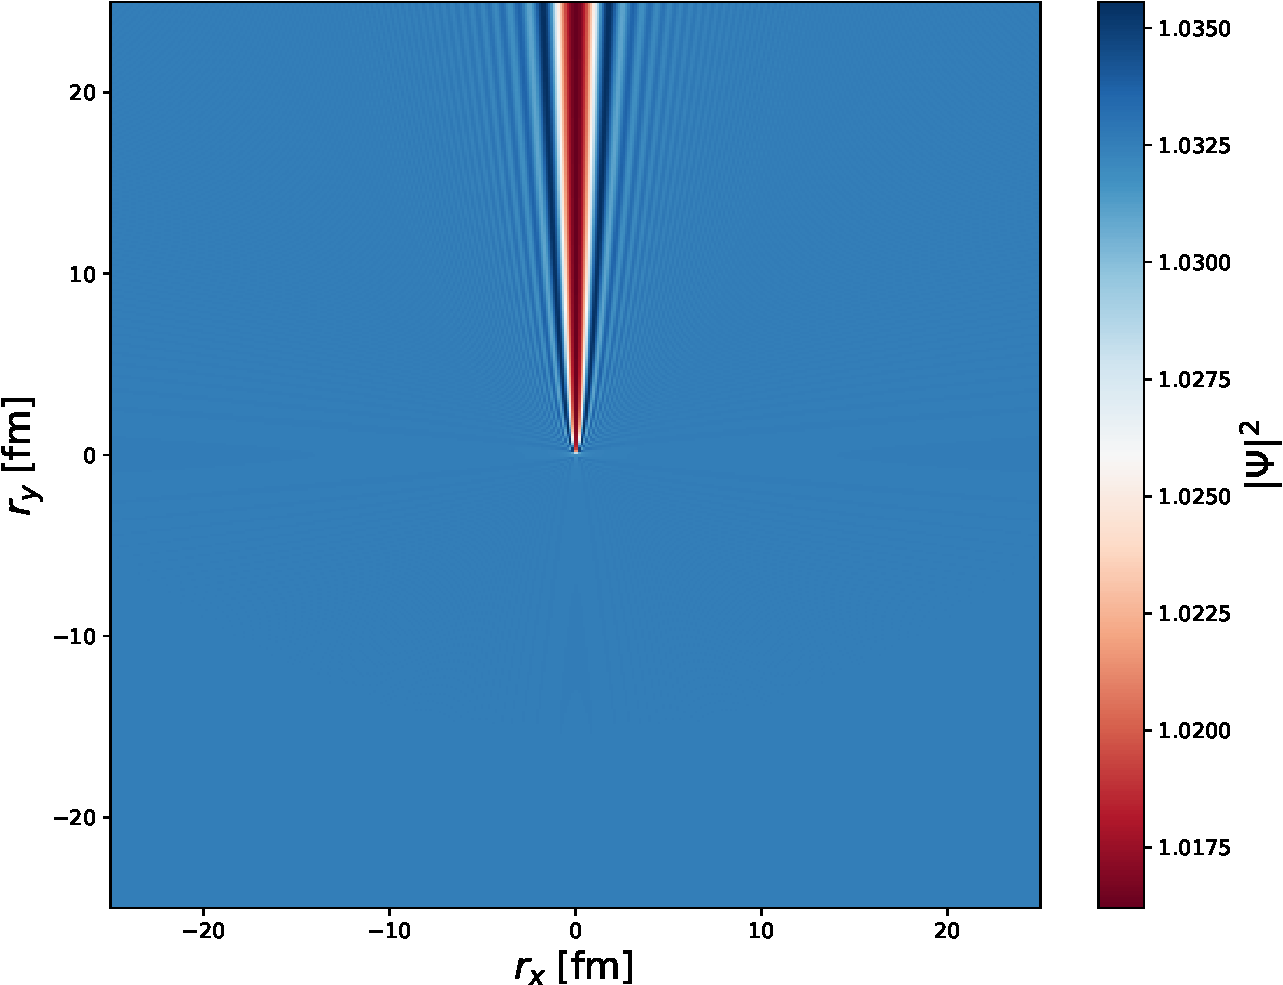
\includegraphics[scale=0.35]{pic/Coulomb/Psi2_rxry_nosym_AbsSQR-cropped.pdf}
\includegraphics[scale=0.35]{pic/Coulomb/Psi2_rxry_sym_AbsSQR-cropped.pdf}
\caption{A kétrészecske Coulomb hullámfüggvény $r_y=0$ metszete a $\bm{k}=(0,0,50)\;\mathrm{MeV}$ momentum esetén. Baloldali ábra a szimmetrizáció nélküli, míg a jobb oldali ábra a szimmetrizált  hullámfüggvényt mutatja. }
\end{figure}

\subsubsection{Háromrészecske}

A háromrészecske Coulomb korrekció meghatározásához a háromrészecske Coulomb problémát kellene megoldani, azaz a következő Schrödinger egyenletet ~\cite{Alt:1998nr}:
\begin{equation}
\Bigg[H_0+\sum_{i<j=1}^3V^{\mathcal{C}}_{ij}(\bm{r}_{ij})
-\sum_{i=1}^3\frac{\hbar^2 k^2_i}{2m_i}
\Bigg]\Psi_{\bm{k}_{12}, \bm{k}_{13}, \bm{k}_{23}}(\bm{r}_{12},\bm{r}_{13},\bm{r}_{23}) = 0,
\end{equation}
azzal az egyszerűsítéssel, hogy azonos részecskékről lévén szó teljesül: $m_i=m$ és $V^\mathcal{C}_{ij}(\bm{r}_{ij})=V^\mathcal{C}(\bm{r}_{ij})=-\frac{1}{4\pi\epsilon_0}\frac{e^2}{\abs{\bm{r}_{ij}}}$ ($\bm{r}_{ij},\;\bm{k}_{ij}$ a relatív változók). Azonban az egyenletnek csupán aszimptotikus egzakt megoldása van. Ezért Bose-Einstein korrelációk vizsgálata során a háromrészecske Coulomb kölcsönhatást úgy vesszük figyelemben, mint három független kétrészecske kölcsönhatást, azaz a hullámfüggvényt a következőképpen állítjuk elő : ~\cite{Alt:1998nr}
\begin{equation}
\Psi_{\bm{k}_{12}, \bm{k}_{13}, \bm{k}_{23}}(\bm{r}_{12},\bm{r}_{13},\bm{r}_{23})  \sim
\Psi_{\bm{k}_{12}}(\bm{r}_{12})\Psi_{\bm{k}_{13}}(\bm{r}_{13})\Psi_{\bm{k}_{23}}(\bm{r}_{23}),
\end{equation}

ahol $\Psi_{\bm{k}_{12}}(\bm{r}_{12})$ a kétrészecske Coulomb probléma megoldása. Tehát a következő Schrödinger egyenletet elégíti ki:
\begin{equation}
\Bigg[-\frac{\hbar^2}{2\mu}\Delta_{\bm{r}_{ij}}+V^\mathcal{C}(\bm{r}_{ij})-\frac{\hbar^2 \bm{k}^2_{ij}}{2\mu}
\Bigg]\Psi_{\bm{k}_{ij}}(\bm{r}_{ij})=0,
\end{equation}
ahol $\mu$ a redukált tömeg (pion tömeg fele), valamint a $\bm{k}_{ij}$ az $i,j$ részecskepár relatív momentumának a fele. Az egyenlet megoldása:

\begin{equation}
\Psi_{\bm{k}_{ij}}(\bm{r}_{kl}) = \mathcal{N}_{ij}e^{i\bm{k}_{ij}\bm{r}_{kl}}F(-i\eta_{ij},1,i(k_{ij}r_{kl}-\bm{k}_{ij}\bm{r}_{kl})),\;\;\;\;\;\;
\mathcal{N}_{ij}=e^{-\frac{\pi}{2}\eta_{ij}}\Gamma(1+i\eta_{ij}),
\end{equation}
ahol $\eta_{ij}=\frac{\mu\alpha}{2k_{ij}}$. Azonban annak érdekében, hogy ezt a megoldást használhassuk a háromrészecske hullámfüggvényben, a következő módosítást kell végrehajtani  ~\cite{Alt:1998nr,Biyajima:2003ey, Mizoguchi:2000km}:

\begin{equation}
\Psi_{\bm{k}_{ij}}(\bm{r}_{kl}) = \mathcal{N}_{ij}e^{i\frac{2}{3}\bm{k}_{ij}\bm{r}_{kl}}F(-i\eta_{ij},1,i(k_{ij}r_{kl}-\bm{k}_{ij}\bm{r}_{kl}))
\label{eq:Psikij}
\end{equation}
\Aref{eq:Psikij} egyenlet által megadott hullámfüggvényt a három relatív koordinátában véve és összeszorozva, valamint a szimmetrizációt elvégezve megkaphatjuk a háromrészecske Bose-Einstein korrelációk vizsgálatánál használt Coulomb hullámfüggvényt:
\begin{equation}
\begin{aligned}
\Psi_{\bm{k}_{12}, \bm{k}_{13}, \bm{k}_{23}}(\bm{r}_{12},\bm{r}_{13},\bm{r}_{23})  = \frac{1}{\sqrt{6}}\Bigg[
\Psi_{\bm{k}_{12}}(\bm{r}_{12})\Psi_{\bm{k}_{13}}(\bm{r}_{13})\Psi_{\bm{k}_{23}}(\bm{r}_{23})+\\
\Psi_{\bm{k}_{12}}(\bm{r}_{23})\Psi_{\bm{k}_{13}}(\bm{r}_{12})\Psi_{\bm{k}_{23}}(\bm{r}_{13})+\\ 
\Psi_{\bm{k}_{12}}(\bm{r}_{13})\Psi_{\bm{k}_{13}}(\bm{r}_{23})\Psi_{\bm{k}_{23}}(\bm{r}_{12})+\\
\Psi_{\bm{k}_{12}}(\bm{r}_{12})\Psi_{\bm{k}_{13}}(\bm{r}_{23})\Psi_{\bm{k}_{23}}(\bm{r}_{13})+\\
\Psi_{\bm{k}_{12}}(\bm{r}_{13})\Psi_{\bm{k}_{13}}(\bm{r}_{12})\Psi_{\bm{k}_{23}}(\bm{r}_{23})+\\
\Psi_{\bm{k}_{12}}(\bm{r}_{23})\Psi_{\bm{k}_{13}}(\bm{r}_{13})\Psi_{\bm{k}_{23}}(\bm{r}_{12})
\Bigg]
\end{aligned}
\end{equation}


\subsection{A Coulomb-korrekciós integrál}

\subsubsection{Kétrészecske}
\Aref{eq:Kn} egyenlet alapján a kétrészecske Coulomb integrál a következő lesz:

\begin{equation}
K(\bm{p}_1,\bm{p}_2)=
\frac{
\iint \mathcal{S}(\bm{p}_1, \bm{r}_1)\mathcal{S}(\bm{p}_2, \bm{r}_2)
\abs{\Psi^{0}_{\bm{p_1},\bm{p_2}}(\bm{r_1},\bm{r_2})} d^3 \bm{r}_1d^3 \bm{r}_2
}{\iint \mathcal{S}(\bm{p}_1, \bm{r}_1)\mathcal{S}(\bm{p}_2, \bm{r}_2)
\abs{\Psi^\mathcal{C}_{\bm{p_1},\bm{p_2}}(\bm{r_1},\bm{r_2}}d^3 \bm{r}_1d^3 \bm{r}_2}
\label{eq:Kn2}
\end{equation}

A kétrészecske Coulomb probléma tárgyalásánál láttuk, hogy célszerű áttérni az $\bm{r}=\bm{r_1}-\bm{r_2}$, $2\bm{R}=\bm{r_1}+\bm{r_2}$, $2\bm{k}=\bm{p_1}-\bm{p_2}$ és $2\bm{K}=\bm{p_1}+\bm{p_2}$ változókra, ekkor ugyanis mind a szabad, mind a Coulomb hullámfüggvény négyzete $\bm{R}$ és  $\bm{K}$ független lesz:
\begin{equation}
\abs{\Psi_{\bm{k},\bm{K}}(\bm{r},\bm{R})}^2 = \abs{e^{i\bm{KR}}\Psi_{\bm{k}}(\bm{r})}^2=\abs{\Psi_{\bm{k}}(\bm{r})}^2,
\end{equation}
így $\bm{R}$ függés csak a forrásfüggvényben marad. Ez azt jelenti, hogy ~\aref{eq:Kn2} Coulomb integrál a következő alakra egyszerűsödik:
\begin{equation}
K(\bm{k},\bm{K})=
\frac{
\int \mathcal{S}_2(\bm{r}, \bm{k}, \bm{K})
\abs{\Psi^{0}_{\bm{k}}(\bm{r})} d^3 \bm{r}
}{\int \mathcal{S}_2(\bm{r}, \bm{k}, \bm{K})
\abs{\Psi^{\mathcal{C}}_{\bm{k}}(\bm{r})} d^3 \bm{r}},
\label{eq:K2}
\end{equation}
ahol a bevezetett $\mathcal{S}_2$ a következőképpen számolható:
\begin{equation}
\mathcal{S}_2(\bm{r}, \bm{k},\bm{K}) = \int \mathcal{S}\Big(\bm{K}+\bm{k}, \bm{R}+\frac{1}{2}\bm{r}\Big)\mathcal{S}\Big(\bm{K}-\bm{k}, \bm{R}-\frac{1}{2}\bm{r}\Big)d^3\bm{R}.
\end{equation}
Ez az integrál elvégezhető, amennyiben a forrást $\alpha, R_M$ paraméterekkel jellemzett Lévy eloszlásnak tekintjük, a végeredmény a következő lesz:
\begin{equation}
\mathcal{S}(\bm{p},\bm{r})=\mathcal{L}(\bm{r},\alpha,R_M)\Longrightarrow \mathcal{S}_2(\bm{r},\bm{k},\bm{K})=\mathcal{L}(\bm{r}, \alpha, 2^{\frac{1}{\alpha}}R_M)
\end{equation}
\subsubsection{Háromrészecske}
\Aref{eq:Kn} egyenlet alapján a kétrészecske Coulomb integrál a következő lesz:
\begin{equation}
K(\bm{p}_1,\bm{p}_2,\bm{p}_3)=
\frac{
\iiint 
\mathcal{S}(\bm{p}_1, \bm{r}_1)\mathcal{S}(\bm{p}_2, \bm{r}_2)\mathcal{S}(\bm{p}_3, \bm{r}_3)
\abs{\Psi^{0}_{\bm{p_1},\bm{p_2}\bm{p_3}}(\bm{r_1},\bm{r_2},\bm{r_2})} d^3 \bm{r}_1d^3 \bm{r}_2d^3 \bm{r}_3
}{\iiint
\mathcal{S}(\bm{p}_1, \bm{r}_1)\mathcal{S}(\bm{p}_2, \bm{r}_2)\mathcal{S}(\bm{p}_3, \bm{r}_3)
\abs{\Psi^\mathcal{C}_{\bm{p_1},\bm{p_2},\bm{p_3}}(\bm{r_1},\bm{r_2},\bm{r_3})}d^3 \bm{r}_1d^3 \bm{r}_2d^3 \bm{r}_3}
\label{eq:Kn3}
\end{equation}

Kétrészecske esethez hasonlóan itt is bevezetjük a relatív koordinátákat, azaz a következő változókra tértünk rá:
\begin{equation}
\bm{r}_{ij} = \bm{r}_i-\bm{r}_j,\;\;\;\;\;\;\;
\bm{R}=\frac{\bm{r}_1+\bm{r}_2+\bm{r}_3}{3},\;\;\;\;\;\;\;
\bm{k}_{ij}=\frac{\bm{p}_{i}-\bm{p}_{j}}{2},\;\;\;\;\;\;\;
\bm{K} = \frac{\bm{p}_1+\bm{p}_2+\bm{p}_3}{3},
\label{eq:CMF3}
\end{equation}
továbbá teljesül $\bm{r}_{23}=\bm{r}_{13}-\bm{r}_{12}$ és $\bm{k}_{23}=\bm{k}_{13}-\bm{k}_{12}$ összefüggés, így az integrálási mérték: $d^3 \bm{r}_1d^3 \bm{r}_2d^3 \bm{r}_3=d^3\bm{R} d^3\bm{r}_{12} d^3\bm{r}_{13}$ lesz. A hullámfüggvények ebben az esetben is csak a relatív változóktól függenek, $\bm{R}$ függése csak a forrásfüggvényeknek lesz, ezért a $d^3\bm{R}$ integrálás ismét a forrásfüggvények szorzatára hat. Így a háromrészecske Coulomb integrál a következő alakú lesz:

\begin{equation}
K(\bm{k}_{12},\bm{k}_{13},\bm{K})=
\frac{
\iint
\mathcal{S}_{3}(\bm{r}_{12}, \bm{r}_{13}, \bm{k}_{12}, \bm{k}_{13}, \bm{K})
\abs{\Psi^{0}_{\bm{k_{12}},\bm{k_{13}}\bm{k_{23}}}(\bm{r_{12}},\bm{r_{13}},\bm{r_{23}})} d^3 \bm{r}_{12}d^3 \bm{r}_{13}
}{\iint
\mathcal{S}_{3}(\bm{r}_{12}, \bm{r}_{13}, \bm{k}_{12}, \bm{k}_{13}, \bm{K})
\abs{\Psi^{\mathcal{C}}_{\bm{k_{12}},\bm{k_{13}}\bm{k_{23}}}(\bm{r_{12}},\bm{r_{13}},\bm{r_{23}})} d^3 \bm{r}_{12}d^3 \bm{r}_{13}},
\label{eq:K3}
\end{equation}

ahol a bevezetett $\mathcal{S}_3$ a következőképpen néz ki (momentum függést nem írtam ki):
\begin{equation}
\mathcal{S}_{3}(\bm{r}_{12}, \bm{r}_{13}) =
\int 
\mathcal{S}\bigg(\bm{R}+\frac{5}{3}\bm{r}_{12}+\frac{1}{3}\bm{r}_{13}\bigg)
\mathcal{S}\bigg(\bm{R}+\frac{2}{3}\bm{r}_{12}+\frac{1}{3}\bm{r}_{13}\bigg)
\mathcal{S}\bigg(\bm{R}-\frac{7}{3}\bm{r}_{12}-\frac{2}{3}\bm{r}_{13}\bigg)
d^3\bm{R}
\end{equation}

A forrásfüggvényre $\alpha,\;R_M$ paraméterekkel rendelkező Lévy eloszlást feltételezve, az összefüggésbe ~\aref{eq:Levyint} definíciót beírva, az $\bm{R}$-re vett integrál elvégezhető, eredményül egy Dirac-deltát ad, így egy további $\bm{q}$-ra vett integrál is elvégezhető, végül a következő alakra egyszerűsödik: 
\begin{equation}
\mathcal{S}_3(\bm{r}_{12}, \bm{r}_{13}) = \frac{1}{(2\pi)^6}
\int
e^{-\abs{\bm{q}_1R_M}^\alpha-\abs{\bm{q}_2R_M}^\alpha-\abs{\bm{q}_1R_M+\bm{q}_2R_M}^\alpha}
e^{-i\bm{q}_1(4\bm{r}_{12}+\bm{r}_{13})}
e^{i\bm{q}_2(3\bm{r}_{12}+\bm{r}_{13})}
d^3\bm{q}_1d^3\bm{q}_2
\label{eq:S3}
\end{equation}


\subsection{Gauss–Kronrod integrálási módszer}\label{sec:GK}

\Aref{eq:Levyint} integrál numerikus kiszámolásához Gauss-Kronrod módszert használtam, mivel ezen módszer használatával érhetünk el nagyon pontos eredményt hatékonyan  ~\cite{LevyEff}. Az integrálás tartománya a teljes tér, amely az cél hiba megadásával végessé tehető a következőképpen: az integrálási tartományt folyamatosan növeljük, amíg hibán belül az érték nem konvergál. 

Az $n$-ed rendű Gauss-kvadratúra $[-1,1]$ tartományon (konvenció szerint ezen a tartományon van megadva a szabály) vett integrált n speciálisan választott pont lineáris kombinációjával becsli:
\begin{equation}
\int_{-1}^1 f(x)dx\approx \sum_{i=1}^n w_if(x_i),
\end{equation}
ahol a $w_i, x_i$ pontok úgy vannak megválasztva, hogy, $2n-1$ vagy ennél alacsonyabb rendű polinomok esetén egzakt eredményt adjon. A módszer jó közelítő eredményt fog adni minden olyan függvényre ami legfeljebb $2n-1$-ed rendű polinommal közelíthető. A formulában szereplő $x_i$ pontok az $n$-ed rendű Legendre polinom gyökei, azaz őket a $P_n(x_i)=0$ egyenlet definiálja, a súlyokat pedig a következőképpen kell meghatározni (\cite{LGQ}):

\begin{equation}
w_i=\frac{2}{(1-x_i)^2(P_n'(x_i))^2}
\end{equation}

Amennyiben az integrálandó függvény $f(x)=\omega(x)g(x)$ alakban áll elő, ahol $g(x)$ egy polinom, akkor új súlyokat vezethetünk be amelyeket az $\omega(x)$ határoz meg, így egy pontosabb közelítő formulát konstruálva. Például ha $\omega(x)=\exp(-x^2)$, akkor a pontokat a Hermite polinom gyökeinek választva és a súlyokat szintén a Hermite polinomokból meghatározva kapunk pontos közelítő formulát $f(x)\exp(-x^2)$ alakú integrál meghatározására (az $f(x)$ itt is legfeljebb $2n-1$-ed rendű lehet).

A Gauss-Kronrod módszer a Gauss módszert egészíti ki, úgy, hogy az $n$-ed rendű Gauss szabály pontjaihoz hozzáad, $n+1$ további pontot, így kapva egy $2n+1$ rendű pontosabb becslést. A módszer lényege, hogy a kevésbé pontos, alacsonyabb rendű módszer pontjait fel lehet használni, egy magasabb rendű módszernél. Az $n+1$ új pont a Stieltjes polinomok (\cite{NIST:DLMF}) határozzák meg. Az alacsonyabb és magasabb rendű becslések közti különbség használható hibabecslésre, amely felhasználható adaptív lépéshossz meghatározásánál (én a munkám során ezt az utat követtem). 


\subsection{Markov-lánc Monte Carlo módszerek}

A Coulomb integrál számítására a Markov-lánc Monte Carlo módszert (\cite{mcbook}) választottuk, mivel ezen módszer segítségével hatékonyabban tudjuk számolni a magas dimenziós integrálokat.

\subsubsection{Monte Carlo módszer}

A Monte Carlo integrálási módszerek tipikusan a következő alakú  $D$ dimenziós integrálok esetén bukkannak fel:
\begin{equation}
I=\int_\Omega f(x)g(x) dx,
\end{equation}
ahol $\Omega$ az integrálási tartomány, $dx$ a $D$ dimenziós integrálási mérték. Amennyiben $\int_\Omega g(x)dx = C$ vezessük be a következő függvényt: $p(x)=g(x)/C$. Triviálisan módon a keresett integrál: 
\begin{equation}
I=C\int_\Omega f(x)p(x)dx \equiv C\langle f \rangle_p,
\end{equation}
ahol  $\langle \cdot \rangle_p$ a $p$ eloszlással számolt várható értéket jelöli.
A $p(x)$ valószínűségi eloszlás szerint válasszunk N pontot a terünkből, ezen pontokat jelöljék $x_1,\dots,x_N\in\Omega$ változók. Ezen minta segítségével becsülhetjük a várható értéket:

\begin{equation}
\bar{I}_N = C\frac{1}{N}\sum_{i=1}^N f(x_i)\equiv C\bar{f}
\label{eq:IN}
\end{equation} 

Mivel az $x_i$-k azonos eloszlású valószínűségi változók, az $f(x_i)$ is azonos eloszlású valószínűségi változó lesz, jelöljük ezt $y_i$-vel. Az új változóban $I/C$ az $y$ várható értéke, $I_N/C$ a várható érték becslése egy $N$ elemű minta alapján. Amennyiben teljesül, hogy $\langle y^4\rangle<\infty$ (vagy $\langle \abs{y}\rangle<\infty$), akkor érvényes lesz a nagy számok erős törvénye, amely alapján a minta várható érték majdnem biztosan tart a várható értékhez:
\begin{equation}
\mathcal{P}\Big(\lim_{N\rightarrow\infty}\bar{I}_N=I\Big)=1,
\end{equation}
ahol $\mathcal{P}$ jelöli a valószínűséget, azaz végtelen sok pontot véve $0$ a valószínűsége, hogy az integrál becslése rossz. Azonban numerikus számolás során valamekkora véges $N$-et kell választanunk, és fontos tudnunk, hogy a pontok számának a növelésével, hogy változik hiba. Ezen kapcsolat meghatározása érdekében az $\bar{I}_{N}$-et tekinthetjük valószínűségi változónak, amelynek van valamekkora $\sigma({\bar{I}_N})$ szórása, amely a következőképpen számolható:
\begin{equation}
\sigma^2({\bar{I}_N})=\frac{C^2}{N^2}\sum_{i=1}^N\sigma^2(f)=\frac{C^2\sigma^2(f)}{N}\Longrightarrow \sigma(\bar{I}_N)=\frac{C\sigma(f)}{\sqrt{N}},
\end{equation}
ahol a $\sigma(f)$ becsülhető a mintából a következő módon:
\begin{equation}
\sigma(f)=\frac{1}{N-1}\sum_{i=1}^N\big(f(x_i)-\bar(f)\big)^2
\end{equation}
Tehát a hiba a pontok számának a gyökével csökken.

Amennyiben $g(x)=1$, egyenletes eloszlással mintavételezhettük és az integrál értéke $I=V\bar{f}$ lesz, ahol $V=\int_\Omega dx$.

\subsubsection{Markov-láncok}

A Monte-Carlo integrálás során lényeges lépés bizonyos eloszlással létrehozni egy mintát. Ennek a megvalósítása az úgynevezett diszkrét Markov-láncok (\cite{norris1998markov}) segítségével történhet. 

\begin{definition}
Az $X_1,\dots,X_N$ ($\Omega$ értékű) valószínűségi változók sorozatát Markov-láncnak nevezzük, ha $\forall n$ és $\forall x_1,\dots,x_{n+1}\in\Omega$ esetén teljesül az úgynevezett Markov tulajdonság:
\begin{equation}
\mathcal{P}(X_{n+1}=x_{n+1}|X_n=x_n,\dots,X_1=x_n)=\mathcal{P}(X_{n+1}=x_{n+1}|X_n=x_n)
\end{equation}
\end{definition}

Tehát egy Markov-lánc egy olyan sztochasztikus folyamat, amelynek nincs memóriája, azaz egy adott időpillanatbeli valószínűség csupán az $1$ lépéssel előtti értéktől függ. 

Markov-láncokra a nagy számok erős törvényéhez hasonló, de annál erősebb, tételt mondhatunk ki, amely lehetővé teszi az ilyen folyamatok alkalmazását a Monte Carlo módszereknél. A tétel megfogalmazása előtt, definiálni kell néhány fontos fogalmat a Markov-folyamatokra.

\begin{definition}
Az $X_1,\dots,X_N$ Markov-láncot homogénnek nevezünk, akkor ha $\forall i,\;\forall a,b\in\Omega: \mathcal{P}(X_{i+1}=a|X_{i}=b)=T_{ab}$. A $T$ mátrixot sztochasztikus mátrixnak szokás nevezni, és $b$-ből az $a$ állapotba való jutás valószínűségét mondja meg  ($\sum_{b\in\Omega}T_{ab}=1$).
\end{definition}

\begin{definition}
Az $X_1,\dots,X_N$ Markov-lánc irreducibilis, ha $\forall a,b\in\Omega$: $\exists i\geq 0$ úgy, hogy $\mathcal{P}(X_i=a|X_{0}=b)>0$ (bármely állapotból bármely állapotba el lehet jutni).
\end{definition}

\begin{definition}
Egy $X_1,\dots,X_N$ Markov-láncban, $a\in \Omega$ elemnek, van periódusa, és ez $k(a)$, ha az elembe való visszatérés $k$ többszörös lépésben történik. Azaz:
\begin{equation}
k(a)=\mathrm{LNKO}\{i>0: \mathcal{P}(X_i=a|X_0=a)>0\},
\end{equation} 
ahol LNKO a legnagyobb közös osztót jelenti.
\end{definition}

\begin{definition}
Egy $X_1,\dots,X_N$ Markov-lánc aperiodikus, ha $\forall a\in\Omega$: $k(a)=1$
\end{definition}

\begin{definition}
Egy $\Omega$-n értelmezett $p$ eloszlás stacionáriusnak nevezünk, ha
\begin{equation}
\sum_{a\in\Omega}p_aT_{ab}=p_b,\;\;\;\;\forall b\in\Omega
\end{equation}
A Markov-folyamatot stacionáriusnak nevezzük, ha $\exists\;p$, azaz az $X_n$ eloszlása időtől független.
\end{definition}

Ezen definíciók felhasználásával már kimondható az Ergodicitás tétel Markov-folyamatokra, amelynek első része  analóg a nagy számok erős törvényével (azonban erősebb annál, hiszen elég ha a függvény integrálja konvergens, nem kell abszolút konvergensnek lennie). A második része fontos állítást tesz a Markov-lánc kezdőpontjának megválasztásával kapcsolatban.

\begin{theorem}{Ergodicitás tétel.}
Legyen $X_1,\dots$ egy irreducibilis, homogén Markov-lánc, melynek stacionárius eloszlása  $p$, ekkor  
$\forall f:\Omega\rightarrow\Sigma ,\;\norm{\langle f\rangle}<\infty$
\begin{equation}
\mathcal{P}\Bigg(\lim_{N\rightarrow\infty}\frac{1}{N}\sum_{i=1}^Nf(X_i)=\langle f \rangle_p\Bigg)=1
\end{equation}
Amennyiben a lánc még aperiodikus is, akkor $\forall a,b\in\Omega$ esetén teljesül: 
\begin{equation}
\lim_{n\rightarrow\infty}\mathcal{P}(X_n=a|X_0=b) = p(a),
\end{equation}
azaz nem számít a lánc kezdőpontja. A tétel feltételeit teljesítő folyamatokat szokás ergodikus Markov-láncnak nevezni.
\end{theorem}


\subsubsection{Metropolis-Hastings algoritmus}

Az ergodicitás tétele alapján, ha tudunk konstruálni egy $p$ stacionárius eloszlással rendelkező homogén, irreducibilis Markov-láncot, akkor Markov láncon számolt időátlag (nagy időkre) majdnem biztosan konvergál az $\langle f \rangle_p=\int_\Omega fp$ várható értékhez.

A Metropolis-Hastings egy olyan algoritmus, amely adott $p$ eloszláshoz tud ergodikus Markov-láncot generálni \cite{Metropolis}. Az algoritmus alkalmazása során először egy javasló függvényt kell megkonstruálni, ezt $Q(x_i|x)$ jelölöm, amely javaslatot add, az $x_i$ pontban levő Markov-lánc következő elemére (adott $x_i$ esetén a lánc következő elemére a javasolt $x$ értéket $Q(x_i|x)$ valószínűséggel választjuk). Ezután a javasolt értéket ~\aref{eq:MHalpha} vagy elfogadjuk, vagy eldobjuk, ekkor a következő elem az aktuális elem lesz. Az algoritmus vázlata vázlata  a következő:

\begin{center}
\begin{algorithm}[H]
Legyen $x_0\in \Omega$\;
 \While{$i=1,\dots,N$}{
 Válasszunk $x$ elemet $Q(x_{i-1}|x)$ eloszlás szerint\;
 Elfogadási valószínűség:
 \begin{equation}
 \alpha = \min{\Bigg\{1, \frac{Q(x_{i-1}|x)p(x)}{p(x_{i-1})Q(x|x_{i-1})}\Bigg\}}
 \label{eq:MHalpha}
 \end{equation}
  \eIf{Egyenletes($0,1$)<$\alpha$}{
   $x_i=x$\;
   }{
   $x_i=x_{i-1}$
  }
 }
 \caption{A Metropolis-Hastings algoritmus.}
 \label{alg:MH}
 \KwOut{$x_1,x_2,\dots,x_N$ minta ($p$ eloszlást követ)}
\end{algorithm}
\end{center}

Amennyiben a javasló függvény szimmetrikus, az algoritmus egyszerűsödik és ~\aref{eq:MHalpha} elfogadási valószínűségből kiesik a $Q$. Ezt az egyszerűbb algoritmust nevezik Metropolis algoritmusnak. A munkám során én a következő szimmetrikus ajánló függvényt választottam:
\begin{equation}
Q(x_i|x) = \frac{1}{\sqrt{2\pi\sigma^2}}e^{-\frac{(x-x_i)^2}{2\sigma^2}},
\end{equation}
tehát $x_i$ pontban levő Markov-lánc következő elemére egy $x_i$ körüli normális eloszlásból húztam javaslatot.

\Aref{fig:MCMC} ábra szemlélteti a Metropolis algoritmus alkalmazását. Először az algoritmus segítségével a Lévy eloszlás karakterisztikus függvénye szerint generáltam egy mintát ($\alpha=1.4,\;R=0.5$), az ábrán látható, hogy a kapott minta szépen követi a céleloszlást. A második ábra mutatja egy függvényre a Metropolis algoritmus által generált minta segítségével számolt Monte Carlo integrálás eredményét különböző mintaméret esetén. Az ábrán körülbelül látható, hogy a minta nagyságának a gyökével csökken a hibája az MCMC integrálásnak.

\begin{figure}[H]
\centering
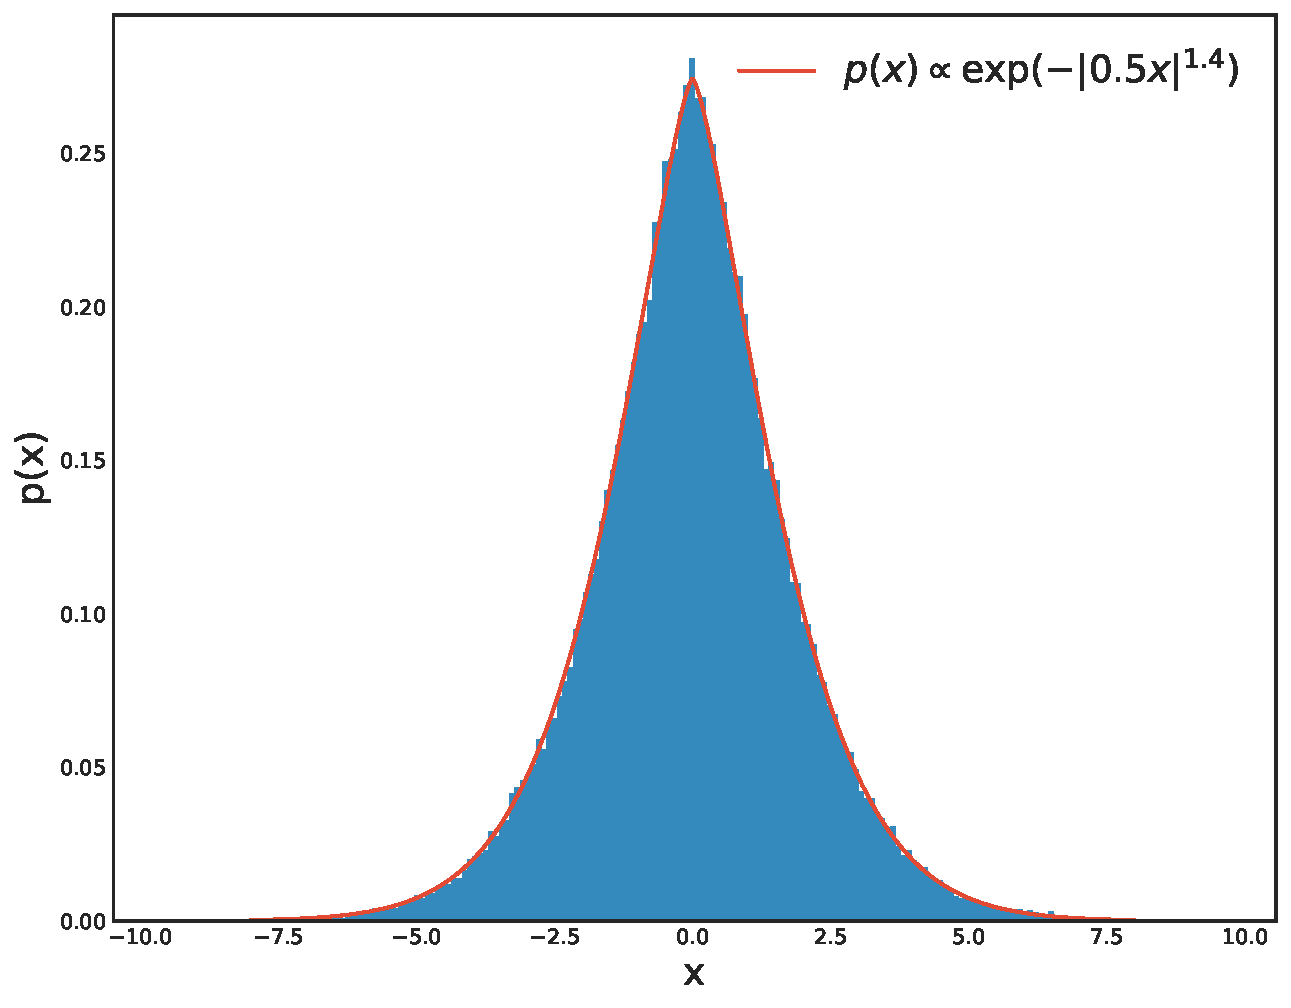
\includegraphics[scale=0.35]{pic/Coulomb/MCSamples.pdf}
\includegraphics[scale=0.33]{pic/Coulomb/MCMCInt.pdf}
\caption{A baloldali ábra mutatja a $p(x)\propto e^{-\abs{0.5x}^{1.4}}$ eloszlással Metropolis algoritmus által generált mintát és céleloszlást. A jobboldali ábra mutatja az Markov-lánc Monte Carlo integrál eredményét a minta nagyságának függvényébe. }
\label{fig:MCMC}
\end{figure}

\subsection{Implementáció}

A Coulomb integrál számolását két lépésben végeztem: először kiszámoltam ~\aref{eq:Levyint} összefüggés által definiált Lévy integrált sok különböző paraméter esetén, majd második lépésben ezen eredményt felhasználva számoltam a Coulomb integrált.

A Lévy integrál számolásához ~\aref{sec:GK} fejezetben bemutatott 15-öd rendű Gauss-Kronrod módszert használtam. Próbálkoztam Markov-lánc Monte Carlo módszerrel is számolni ezen integrált, de a Gauss-Kronrod sokkal hatékonyabb és pontosabb eredményt adott. ~\Aref{eq:LevyintR} összefüggés alapján elegendő a számolást $R=1$ esetén elvégezni, az eredményből aztán bármely másik $R$ paraméter esetén meghatározható az integrál értéke. ~\Aref{eq:LevyintO} összefüggés alapján az integrál értéke csupán az $\bm{r}$ vektor hosszától függ, az iránytól nem, ezért választhatjuk a $\bm{r}=(0,0,r)$ vektort a számolás során, így a z integrál a következő alakra egyszerűsödik:

\begin{equation}
\mathcal{L}(r, \alpha, R) = \frac{1}{2\pi^2}\int_0^\infty \frac{q\sin{qr}}{r}e^{-|qR|^\alpha}dq
\end{equation}

Az integrálás során a lépésközt (azaz a $dq$-t) adaptívan határoztam meg, úgy, hogy a hibát a 7 pontú Gauss szabály és a 15 pontú pontosabb becslés különbségével közelítettem. Az integrálást mind CPU párhuzamos, mind GPU párhuzamos verzióban implementáltam. A saját implementáció mögötti motiváció abból az egyszerű tényből ered, hogy mivel rengeteg sok pontban kell kiszámolnom az integrált ($10^6$ nagyságrendű különböző paraméter esetén), saját implementációval nagyon erősen ki tudom használni a sokmagos architektúrák nyújtotta előnyöket. Továbbá azért döntöttem a grafikus processzorra (GPU) való implementálás mellett is, mert a GPU sokkal nagyobb része van számításra tervezve mint a CPU-é (több tranzisztor vesz részt a számolásban), sokkal több maggal rendelkezik (tipikusan egy modern CPU 4-6, míg egy GPU több ezer maggal), amelyek kihasználhatók a sok integrálás párhuzamos végzése során. Az általános tapasztalatom, az, hogy a GPU bevonása a számolásba költséges, használata csupán a masszívan párhuzamosítható problémák esetén érdemes (konkrétan 128 darab integrál elvégzésig a laptopomban levő 4 magos Intel i7 processzor gyorsabb volt, mint az Nvidia Geforce 960m videokártyán történő számolás, azonban 128 fölött a GPU már győzelmet aratott).

A CPU párhuzamos változat implementálását C++ nyelven végeztem, a legújabb, 2014-es nyelvi standardot követve, amely tartalmazza a CPU-ra történő párhuzamosításhoz szükséges eszközöket. A GPU általános számítás célú programozására több lehetőség van. Nvidia kártyák esetén a leghatékonyabb választás az Nvidia saját fejlesztésű CUDA platformja. De használható erre a célra a más gyártók eszközeit is támogató OpenCL is, viszont általában hosszú és átláthatatlan kódot eredményez. Azonban napjainkban a mesterséges intelligencia térhódításának köszönhetően, kiemelkedő szerephez jutottak a nagy teljesítményű, GPU-t kihasználni tudó könyvtárak. A legbiztatóbb jövőt mutató könyvtár a SYCL, amelynek a szabványát a Khronos csoport definiálta, és ipari szintű implementációja jelenleg béta státuszban van. Ezen könyvtár egy modern C++ absztrakciós réteg az OpenCL-hez, így több gyártó eszközén használható a számítások gyorsításra, miközben az OpenCL hátrányait kiküszöbölve, elegáns kódot eredményez. Mivel én Nvidia GPU-val rendelkezek, ezért a GPU párhuzamosításra CUDA könyvtárat választottam. Következő alfejezetben ezen könyvtár működését mutatom be röviden. 

 
\subsubsection{CUDA}\label{sec:CUDA}
A GPU elsősorban grafikus alkalmazások számára van kifejlesztve. Ezen alkalmazások közös jellemzője, hogy nagyon nagy számítási igényűek és masszívan párhuzamosíthatók. A grafikus processzorokat ennek szellemében fejlesztik. Ennek eredményeként sokkal több tranzisztort dedikálnak számoláshoz, mint a CPU. Az Nvidia ismerte fel először, hogy hardverükben nagy lehetőségek rejlenek a számítás-intenzív, nem grafikus programok számára is, amelyek a tudományos világban folyton felbukkannak. Ezért alkották meg a CUDA platformot, amely egy olyan kiegészítést ad elsősorban C, C++ nyelvekhez, amely segítségével a grafikus processzor általános célú számításra használható. 

CUDA felhasználásával hibrid kódot fejleszthetünk, melyet az Nvidia saját, nvcc névre keresztelt fordítójával tudunk lefordítani. Ezen kódokat azért szokás hibridnek nevezni, mert mind a GPU mind a CPU kódot egy helyen tartalmazzák. A GPU önmagában csak nagyon egyszerű feladatokat tud ellátni (pl. kiszámolni sok integrált), működését a CPU vezérli, ezért a CUDA kódban, a számítások végzésére úgynevezett kerneleket írunk (kb. egy függvény), standard C++ nyelven (STL könyvtár nem használható), amelyeket aztán a CPU-n futó kód tud indítani. A grafikus processzorok saját memóriával rendelkeznek, és a kernelek ezen tudnak operálni. Ez azt jelenti, hogy egy CUDA programban a következő szisztéma szerint kell kódot fejleszteni (ezt szemlélteti ~\aref{fig:cuda} bal oldali ábrája):  
\begin{itemize}
\item Előkészítjük az adatokat, melyeket a CPU-hoz tartozó memóriába tárolunk.
\item Lefoglaljuk a GPU memóriájában a váltózóinknak a helyet a cudaMalloc függvény segítségével. A foglalás után a CPU-n futó programrész printerekkel rendelkezik a lefoglalt helyekre.
\item Az adatokat amelyek szükségesek a GPU-n végzett számításhoz, átmásoljuk a GPU memóriájában lefoglalt helyekre. A másolást a CPU végzi, a cudaMemcpy függvény hívásának következtében.
\item A GPU-ra szánt függvényt (azaz kernelt) meghívjuk, hívás közben megadjuk hogy hány példányban szeretnénk elindítani párhuzamosan és átadjuk a GPU memóriájába lefoglalt helyekre mutató változókat. A kernelek indítása nagyon hasonló a megszokott függvényhíváshoz, csupán annyi az eltérés, hogy függvény neve után \(<\!\!<\!\!<\)\dots\(>\!\!>\!\!>\) alakban specifikálni kell az indítási információkat (hány példányba fusson párhuzamosan). A számolás eredményét a kernelek szintén a GPU memóriájába tudják írják.
\item A számolás eredményét átmásoljuk a GPU memóriájából a CPU memóriájába.
\end{itemize}  

A kernel indításánál \(<\!\!<\!\!<\) és \(>\!\!>\!\!>\) szimbólumok közé kell írni a kernel indításának leírását. A leíráshoz két paramétert kell megadni: blokkok száma és szálak száma blokkonként. Ez mutatja, hogy a CUDA programozási modellje, a párhuzamosan futó szálakat blokkokba csoportosítja. Az Nvidia kártyákban a magok szintén hardveresen blokkokba vannak csoportosítva, ezeket streaming multiprocessornak (SM) nevezik, és a magok mellett tartalmaznak vezérlő áramköröket. Egy blokk egy SM-en fog futni, tetszőleges sorrendben, azaz nem biztos hogy párhuzamosan, hiszen a blokkok száma nincs korlátozva. Amennyiben több blokkot adunk meg mint amennyi SM van a grafikus processzorunkban, akkor hardveresen meg van oldva, hogy ezek egymás után szét legyenek osztva, úgy, hogy mindig kihasználja az adott hardver képességét. Ez gyakorlatilag azt jelenti, hogy a GPU-ra írt kód úgymond erősen skálázik. Tehát megírunk egy kódot, aztán a grafikus processzor belsőleg úgy fogja szétosztani a számolást, hogy mindig teljesen ki legyen használva a hardver. Ezt hivatott szemléltetni ~\aref{fig:cuda} jobb oldali ábra: 8 blokk egy 2 SM-el rendelkező hardver esetén 4-4 blokk csoportra lesz szétosztva, és ezeket egymás után a hardver küldi az SM-eknek, 4 SM-el rendelkező hardver esetén pedig 2-es csoportokba osztja a blokkokat. Ezen működés pedig a GPU architektúrájába van építve. A blokkok számával ellentétbe a szálak száma korlátozott, az újabb eszközökén maximálisan 1024 szál indítható blokkonként. Minden blokkhoz és minden szálhoz tartozik egy egyedi azonosító, egy ID (akárcsak egy ciklus esetén a futó index), ezen azonosítókat minden futó kernel ismeri.

\begin{figure}[H]
\centering
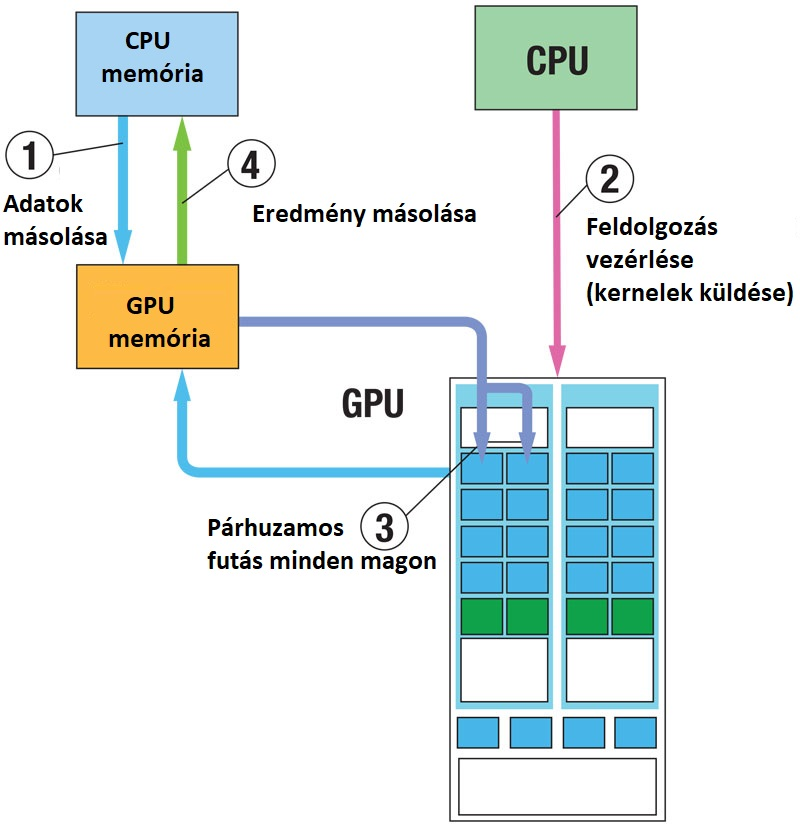
\includegraphics[scale=0.32]{pic/prog/cudamodel}
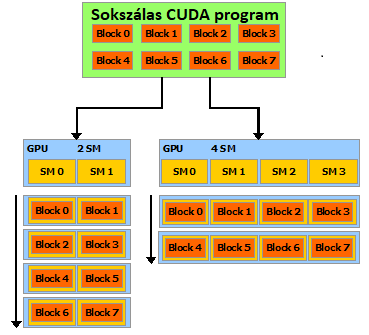
\includegraphics[scale=0.8]{pic/prog/cudascale}
\caption{Baloldali kép: a CUDA program általános felépítését láthatjuk. Jobb oldali kép: CUDA-ban írt programok skálázását mutatja be. (Forrás: internet) }
\label{fig:cuda}
\end{figure}

\subsubsection{MapReduce programozási modell}\label{sec:MapReduce}

A MapReduce egy általánosan használt, egyszerű programozási modell, amelyet párhuzamos adatfeldolgozásra lehet használni. A modell két fő részből épül fel: map és reduce, amely két magasabb rendű függvény (azaz olyan függvények amelynek paraméteri lehetnek függvények). A map függvény mint a neve sugallja egy leképzést végez, alkalmazza az adatokra a kapott függvényt (érezhető módon ez triviálisan párhuzamosítható). A reduce pedig a kapott adatokat a kapott függvény szerint összefűzi (összegzi). Ezen két roppantul hasznos függvénynek sok hasznos implementációja van. Például a map-nek python nyelven az ipyparallel könyvtárban található a klaszter-párhuzamos implementációja, amely a leképzést egy egész klaszteren végzi. 

A Coulomb integrálok számolásánál ezen modell szerint jártam el. Első lépésben az integrál fejlesztettem egy az integrálokat számoló C++ könyvtárat, amelyből egy python csomagot készítettem. Ezután az ipyparallel csomag felhasználásával python nyelven ezen csomagot a MapReduce modell keretében a Brookhaven nemzeti laboratórium egyik klaszterén szétosztva használtam. Azaz először az integrálási paramétereket csoportosítottam kis csomagokba, úgy, hogy annyi csomagot állítsak elő amennyi számítógép áll rendelkezésemre(tipikusan 200-300 gépet használtam), aztán a klaszter-párhuzamos map segítségével elvégeztem az integrálást (egy csomag esetén a leképzés: csomag minden elemére Coulomb integrál kiszámolása). Végül a kapott eredményt reduce függvény segítségével összefűztem, így előállt eredmény egyszerűbb struktúrába került. A programozási modellt ~\aref{fig:mapreduce} ábra szemlélteti.

A MapReduce programozási modell nem csak az integrálás során jött elő, hanem az adatanalízis során is. Ugyanis itt a rendelkezésre álló adatokat szétosztva sok gépre párhuzamosítva meghatároztam a korrelációs függvényt (map), aztán a sok különböző eredményt összefűztem (reduce).

\begin{figure}[H]
\centering
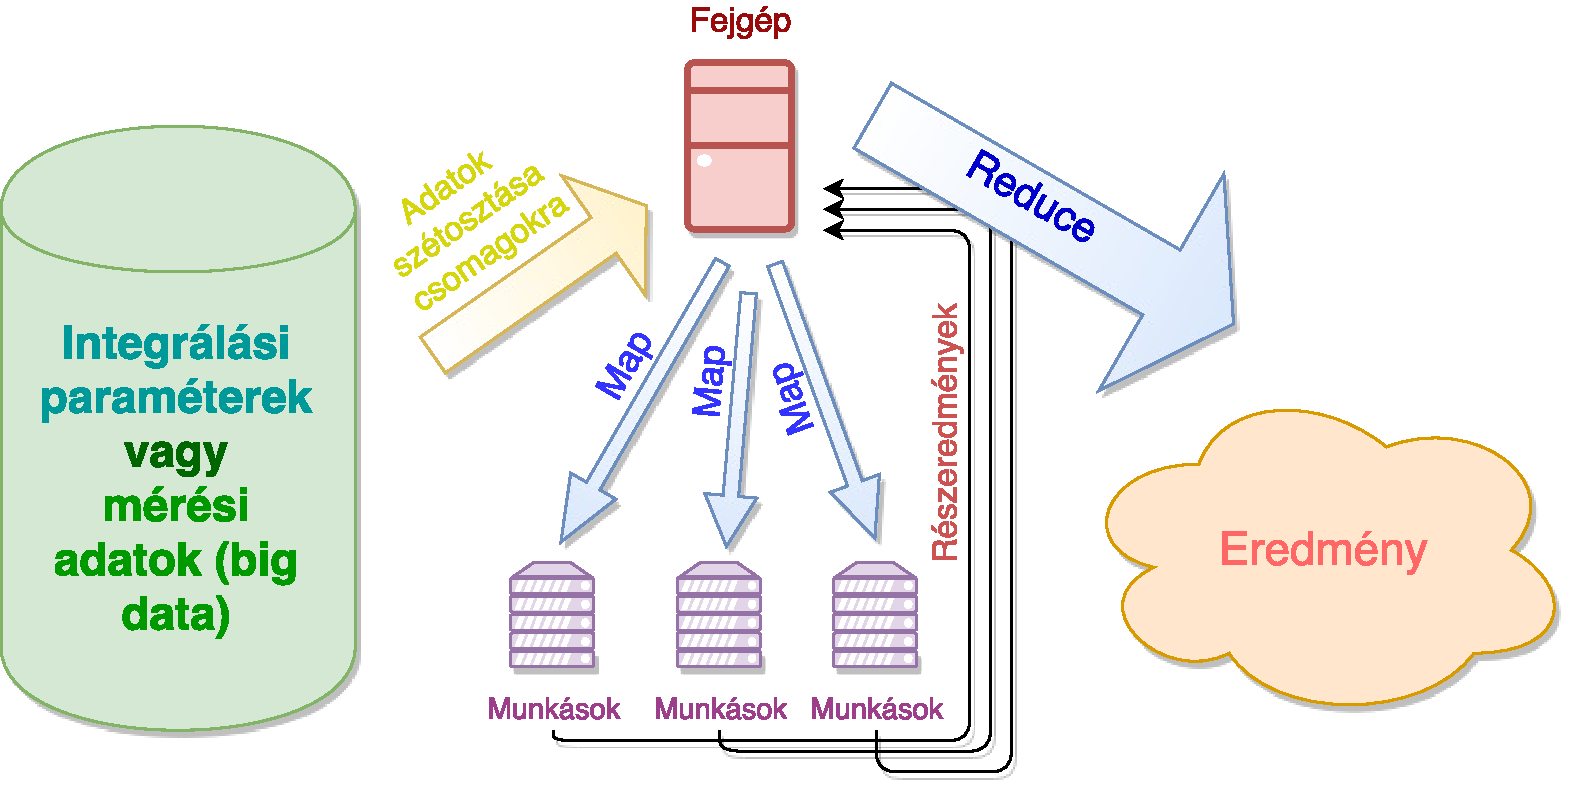
\includegraphics[scale=0.4]{pic/prog/MapReduce}
\caption{Az ábra a MapReduce programozási modellt mutatja be. A fejgép kisebb csomagokra osztja az adatokat, majd a klaszter számítógépein (munkások) elindít egy párhuzamos leképzést egy adott függvénnyel az adatokon (map). Végül a kapott eredményeket a fejgép összefűzi (reduce) és így előáll a végeredmény. }
\label{fig:mapreduce}
\end{figure}



\subsection{Eredmények}

\subsubsection{Teszt: Coulomb kölcsönhatás nélküli eset}

A számolás elvégzésére írt kódot modulárisan fejlesztettem, minden modult külön teszteltem. Minden elvégzett teszt bemutatása hosszadalmas lenne, ezért itt két tesztet mutatok be. 

Az első teszt egy modul kivételével az össze modul megbízhatóságát mutatja (az egy kieső modul a komplex hipergeometrikus függvényt számoló kód, ezt a python mpmath könyvtár segítségével teszteltem). Amennyiben ~\aref{eq:K2} kétrészecske integrál nevezőjét tekintjük, felismerhetjük a korrelációs függvény definícióját, Coulomb kölcsönhatás nélküli esetben. Ez Lévy eloszlást feltételezve forrásfüggvénynek, ~\aref{eq:CHC2} összefüggés alapján a Lévy karakterisztikus függvénye lesz. Az eredményt ~\aref{fig:CRT} ábra szemlélteti. Látható, hogy a numerikus eredmény kellően pontosan reprodukálja az analitikusat.


\begin{figure}[H]
\centering
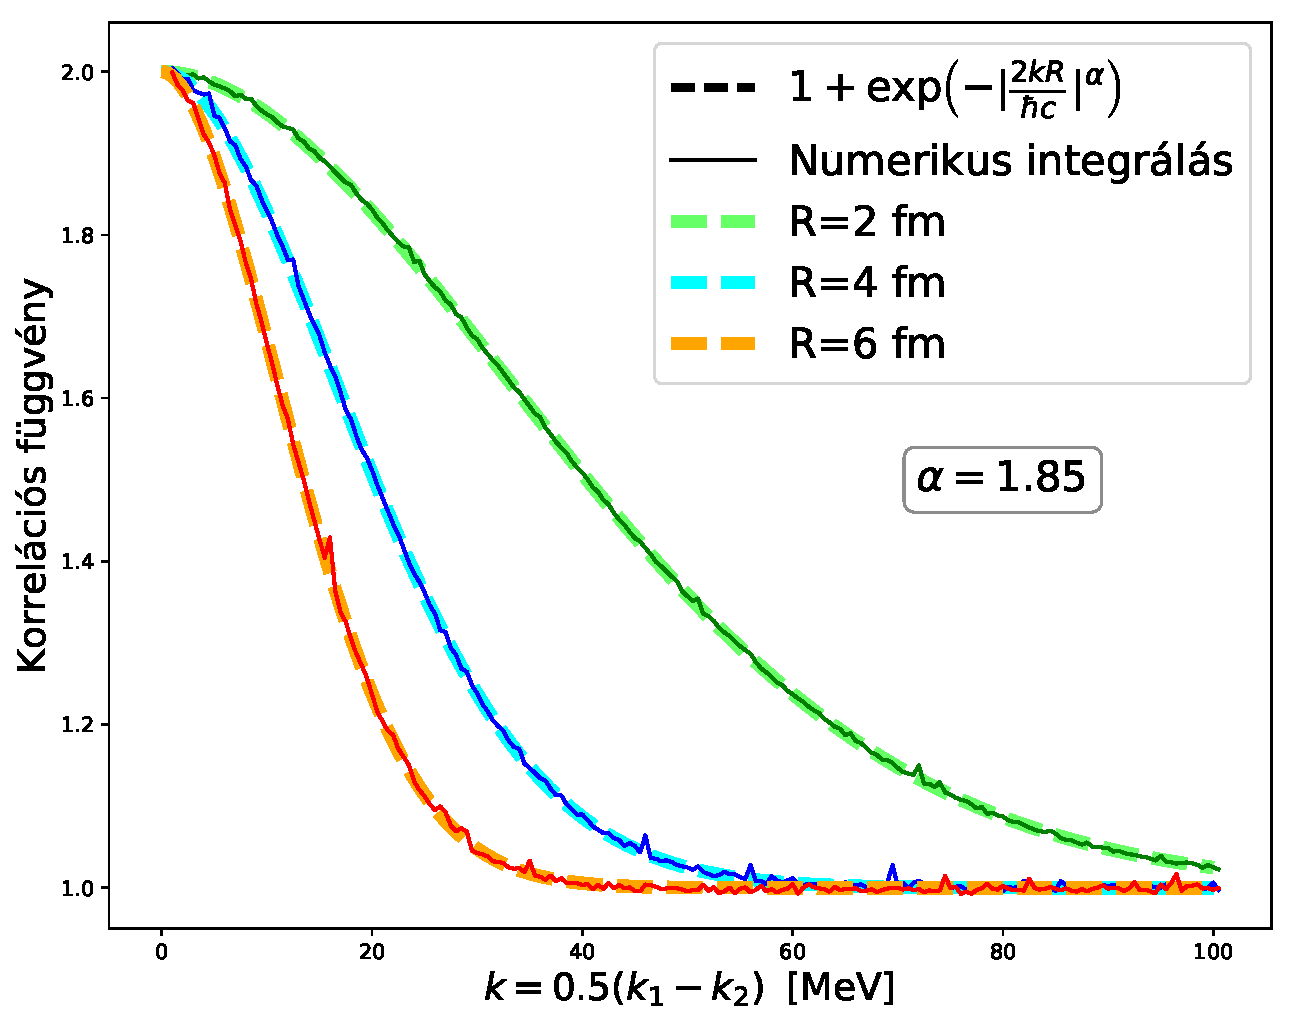
\includegraphics[scale=0.36]{pic/Coulomb/C2_noCoulomb_R246_a185.pdf}
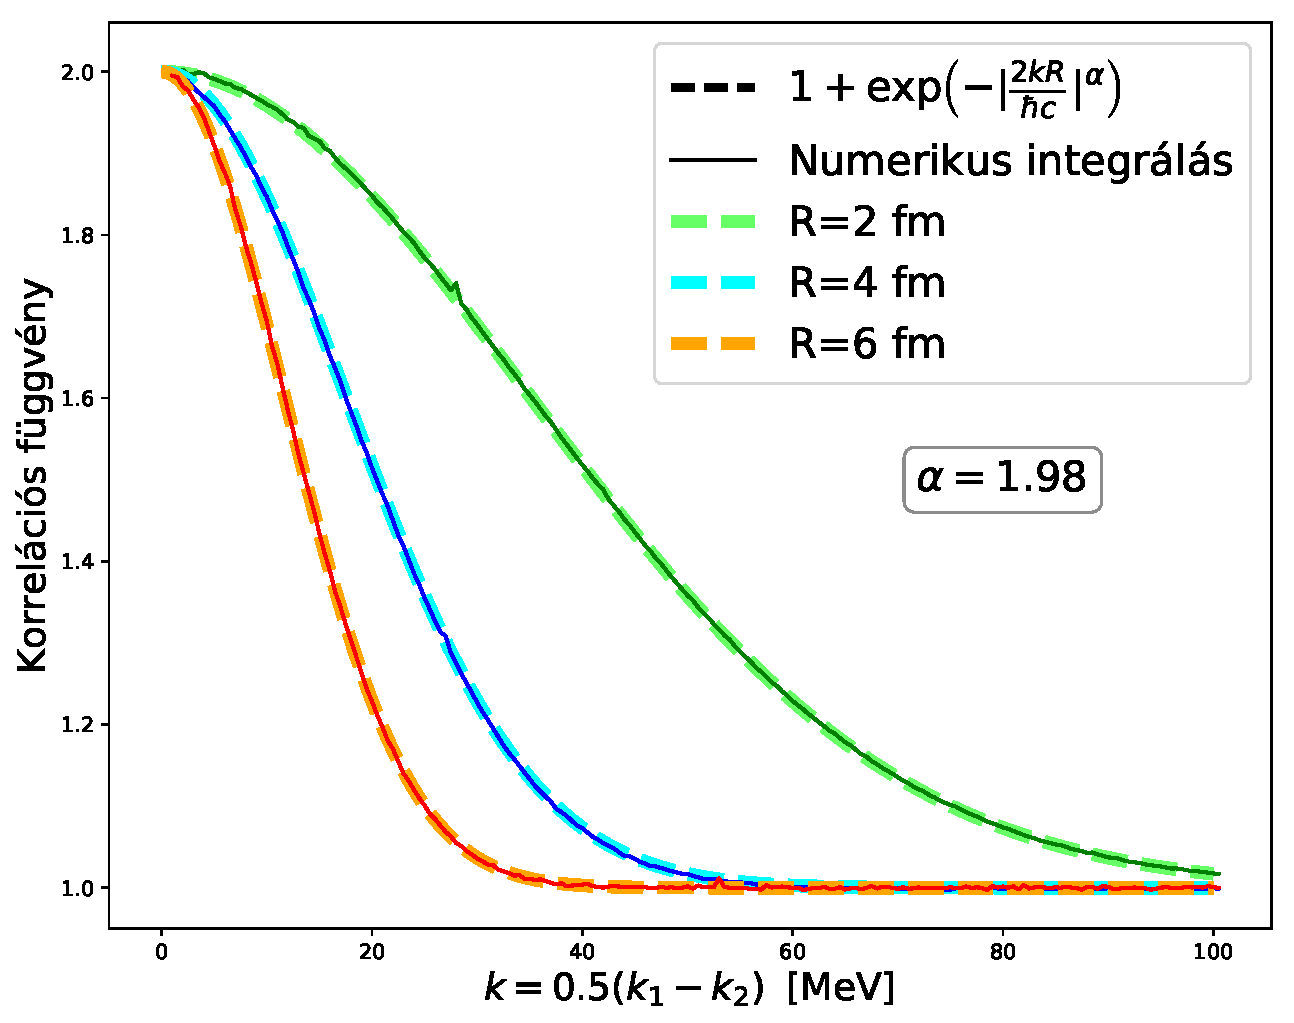
\includegraphics[scale=0.36]{pic/Coulomb/C2_noCoulomb_R246_a198.pdf}
\caption{Coulomb kölcsönhatás nélküli kétrészecske korreláció számolása numerikusan és analitikusan, a kód tesztelése céljából.}
\label{fig:CRT}
\end{figure}


A PHENIX magyar csoport már régóta foglakozik Bose-Einstein korrelációk vizsgálatával, ezért a Coulomb integrál betáblázatozása több körben megtörtént. Jelenleg a legutóbbi számolás eredményeként született táblázat van használatban, amelyet a Nagy Márton készített. Ezt fel lehet használni az általam készített kód tesztelésére. Az összehasonlítás ~\aref{fig:nmc} ábrán látható. Az ábra mutatja, hogy maximálisan $1\%$ a relatív eltérés a két számolás között, ez elfogadható.

\begin{figure}[H]
\centering
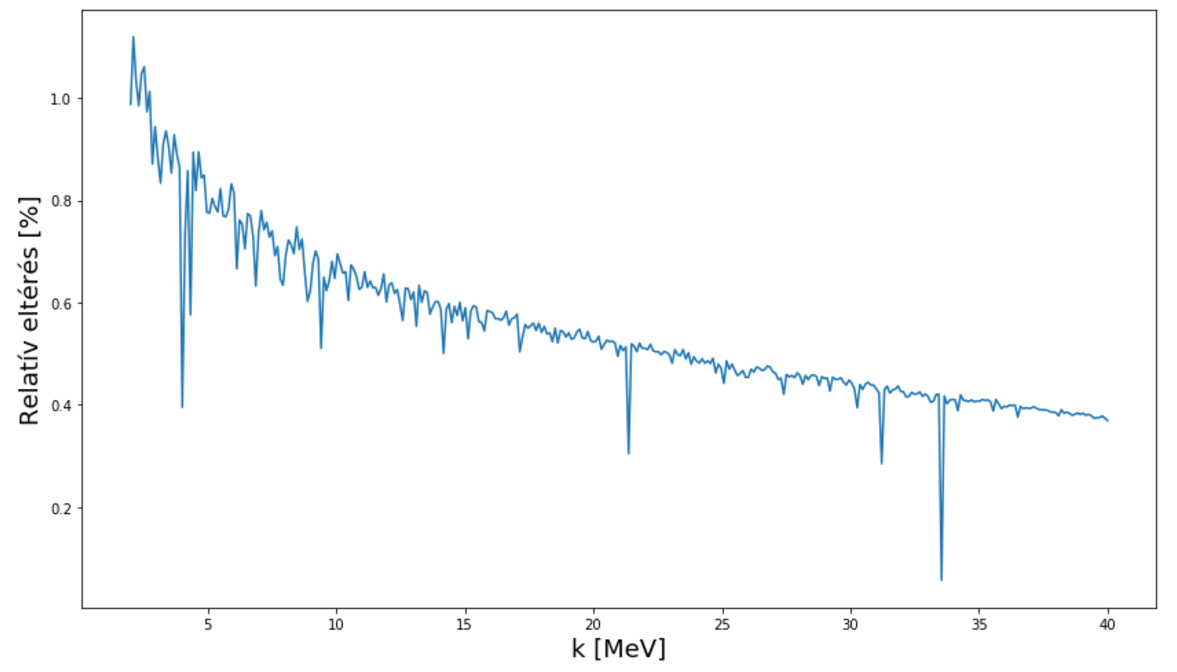
\includegraphics[scale=0.6]{pic/Coulomb/mynm}
\caption{A fejlesztett kód tesztelése a Nagy Márton által számolt Coulomb integrál összehasonlítása révén.}
\label{fig:nmc}
\end{figure}

\subsubsection{Kétrészecske Coulomb korrekció}

A kétrészecske Coulomb integrál relatív impulzus különbség felétől való függését különböző $R$ Lévy paraméter esetén ~\aref{fig:CRK2dR} ábra szemlélteti. Hasonlóan az $\alpha$ Lévy paramétertől való függést \aref{fig:CRK2dalpha} ábra mutatja.

\begin{figure}[H]
\centering
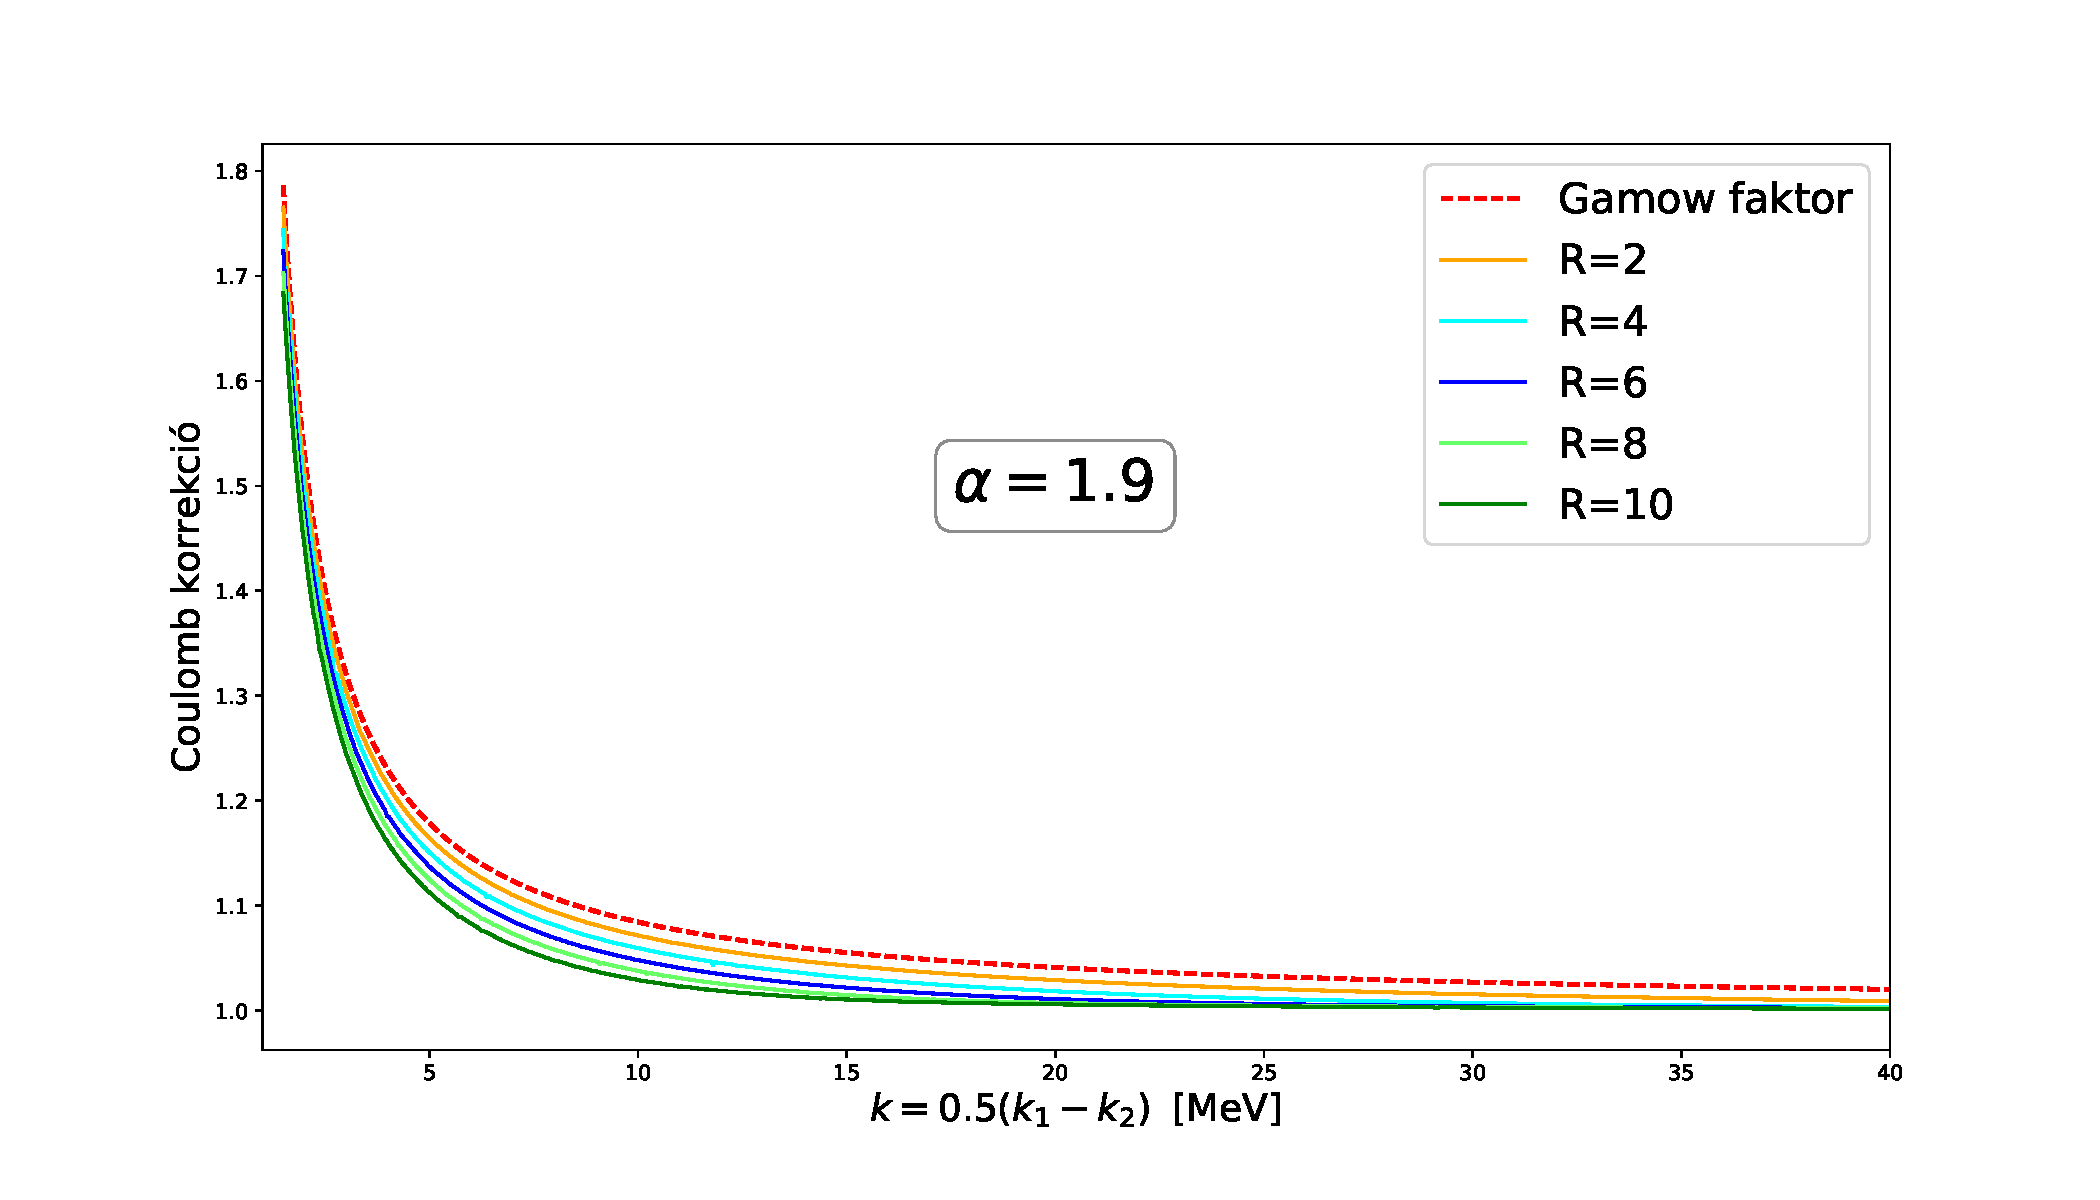
\includegraphics[scale=0.45]{pic/Coulomb/C2_dR_a19_S2correct.pdf}
\caption{Kétrészecske Coulomb korrekció a Lévy eloszlás $R$ paraméterének függvényében. A szaggatott vonal mutatja ~\aref{eq:Gamow} egyenlet által definiált Gamow faktort.}
\label{fig:CRK2dR}
\end{figure}

\begin{figure}[H]
\centering
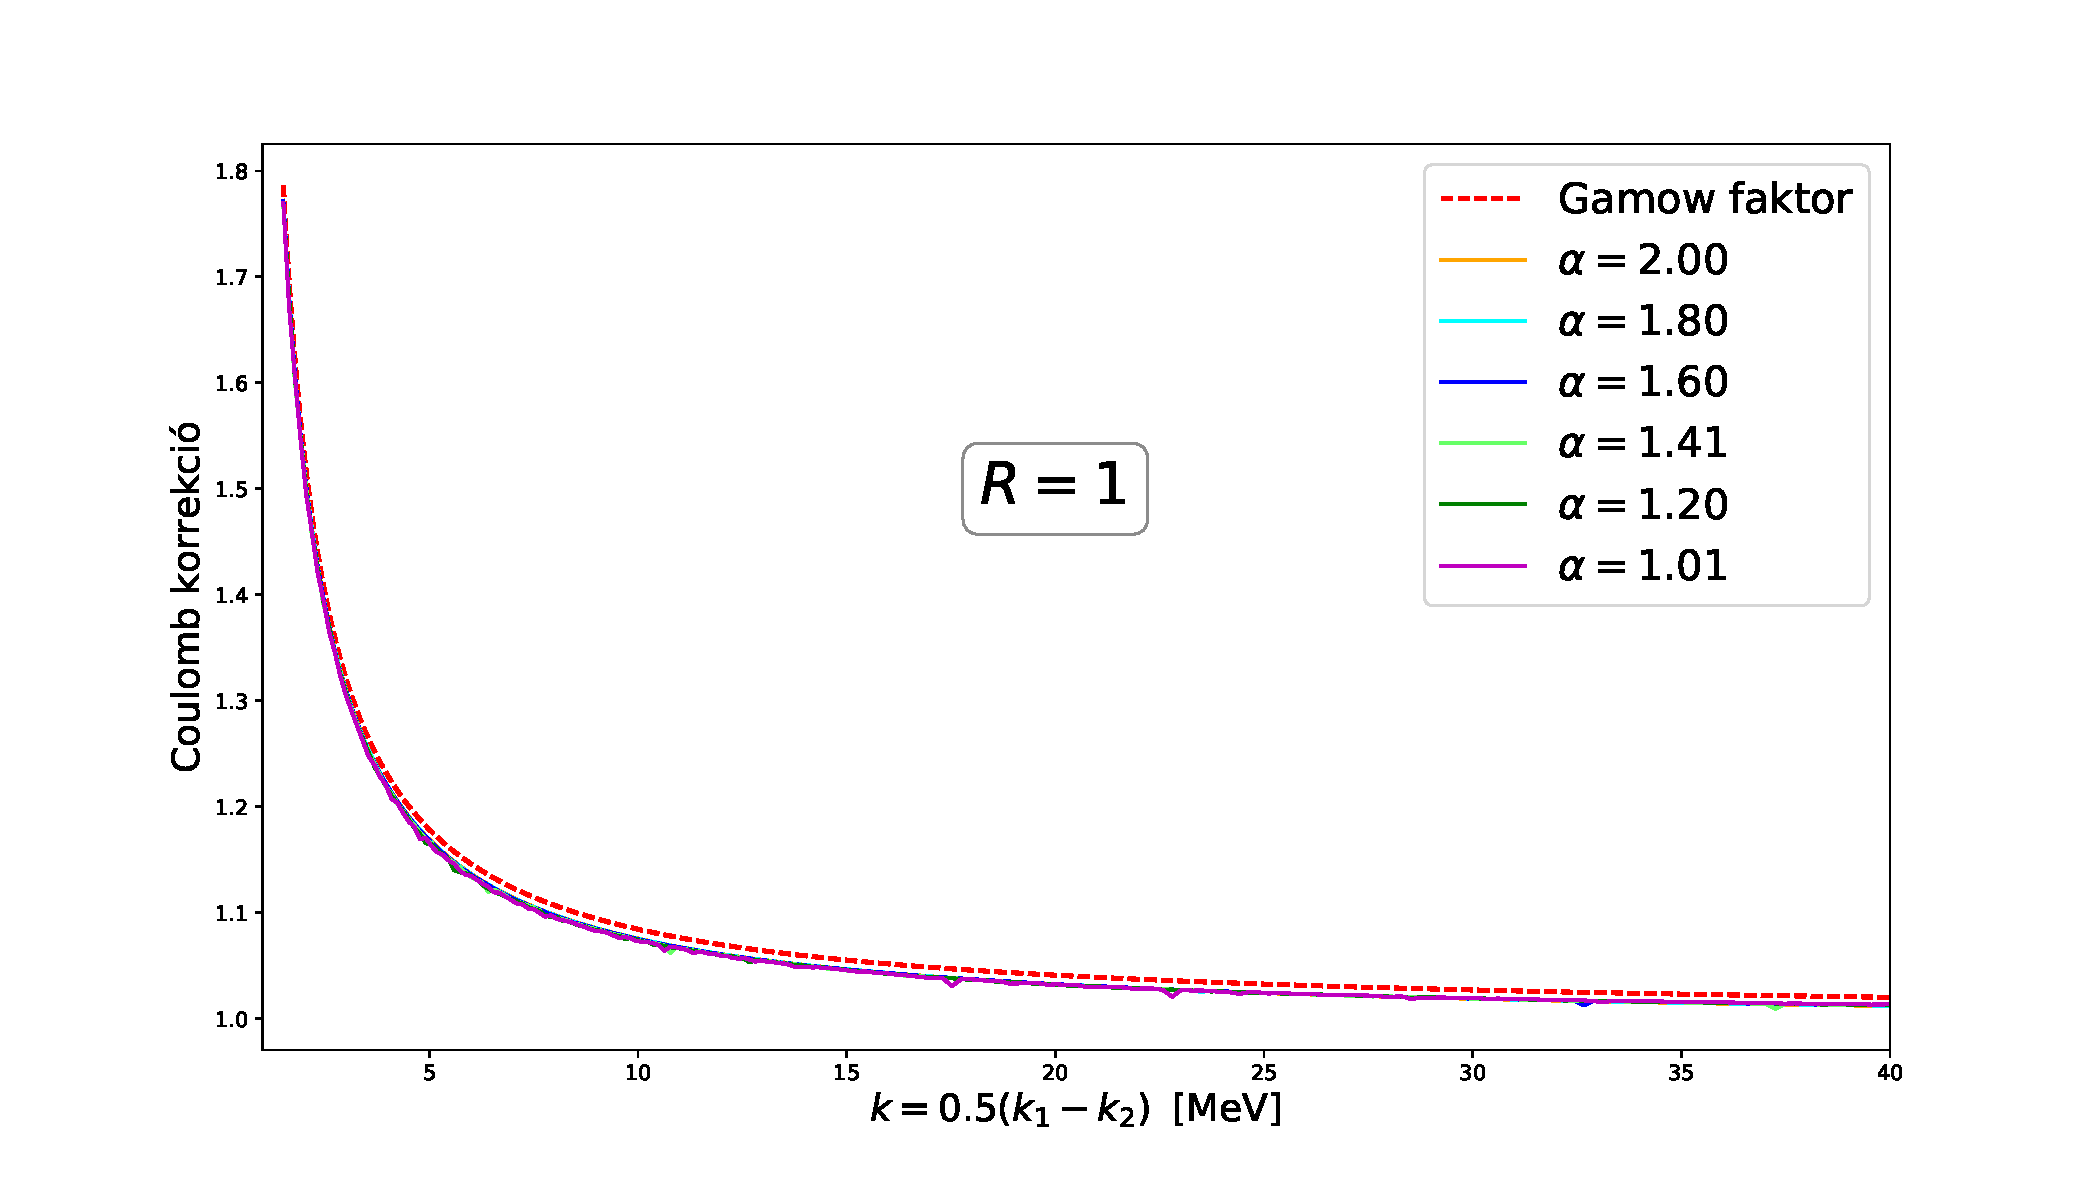
\includegraphics[scale=0.45]{pic/Coulomb/C2_dalpha_R1_S2correct.pdf}
\caption{Kétrészecske Coulomb korrekció a Lévy eloszlás $\alpha$ paraméterének függvényében. A szaggatott vonal mutatja ~\aref{eq:Gamow} egyenlet által definiált Gamow faktort.}
\label{fig:CRK2dalpha}
\end{figure}

\subsubsection{Háromrészecske Coulomb korrekció}

Háromrészecske Coulomb integrál számolásához először meg kell határozni ~\aref{eq:S3} integrált, amely megadja a 3 részecske forrásfüggvényt. Azonban kétrészecske esetén ~\aref{fig:CRK2dalpha} ábra szerint a Coulomb integrál nem függ a Lévy eloszlás $\alpha$ paraméterétől, ezért az $\alpha=2$ közelítést alkalmazzuk az $\mathcal{S}_3$ kiszámolásához. Ekkor a Lévy eloszlás a jól ismert Gauss eloszlás lesz, amelyre analitikusan ki tudjuk számolni az $\mathcal{S}_3$ integrált.

\begin{figure}[H]
\centering
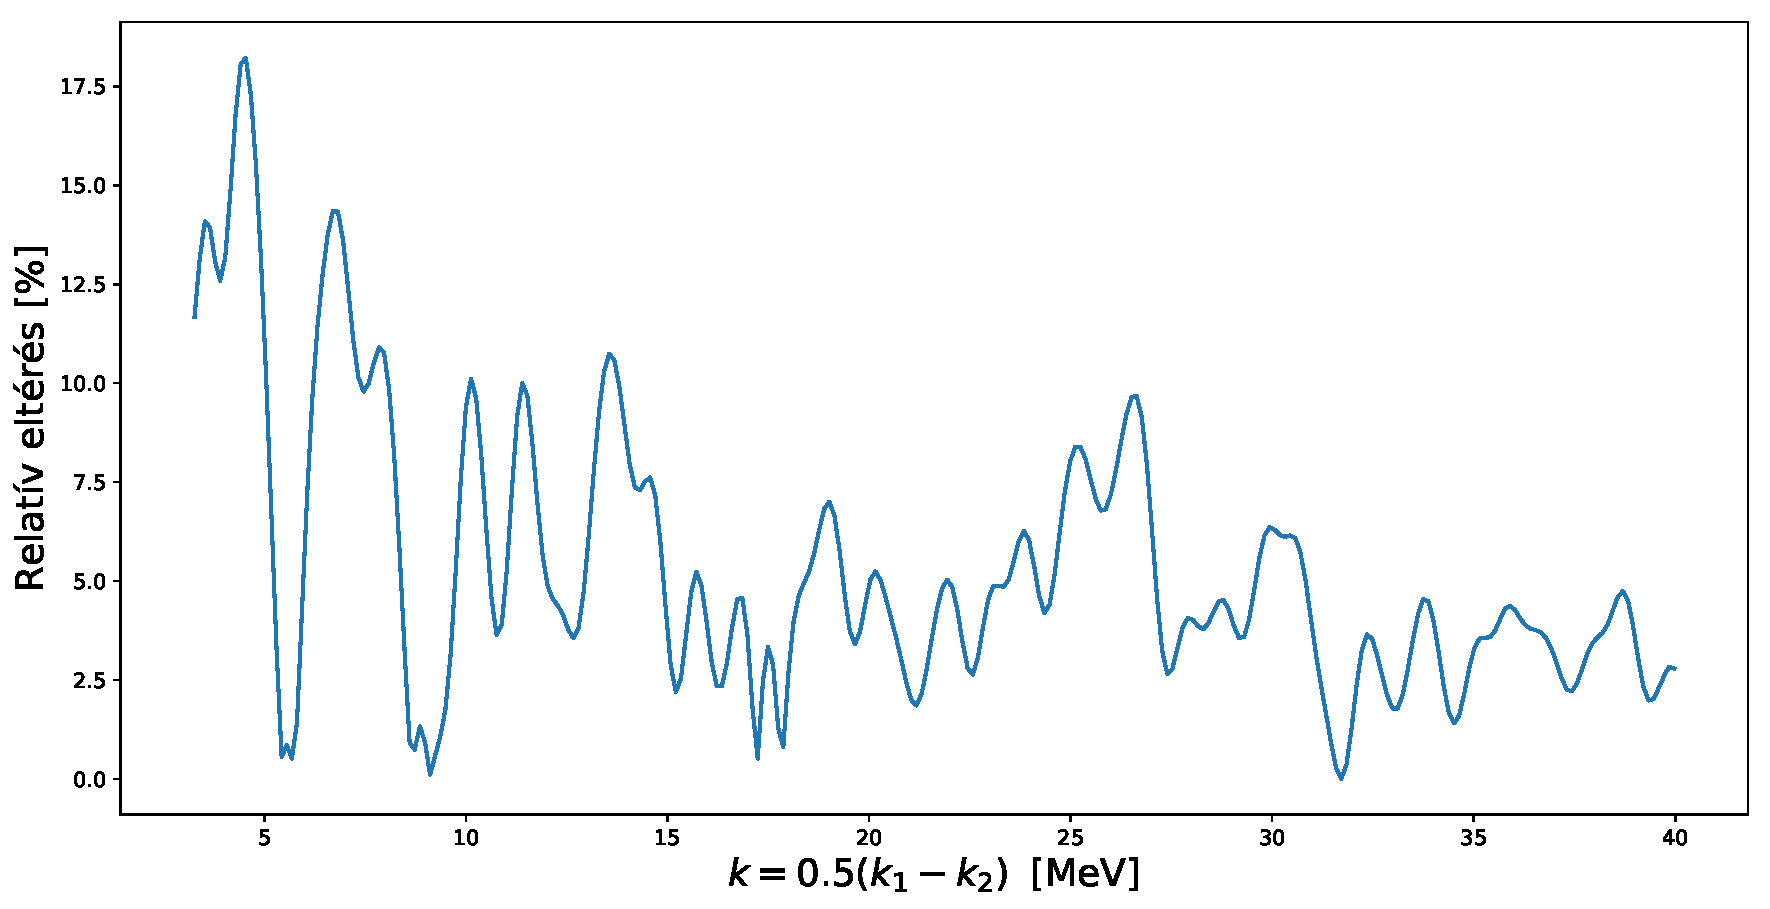
\includegraphics[scale=0.5]{pic/Coulomb/K3_error2.pdf}
\end{figure}
%Ha azt mondhatnánk, hogy $\abs{\bm{q}_1R_M+\bm{q}_2R_M}^\alpha\approx \abs{\bm{q}_1R_M}^\alpha+\abs{\bm{q}_2R_M}^\alpha$, akkor az $\mathcal{S}_3$ a következő lenne:
%\begin{equation}
%\mathcal{S}_3(\bm{r}_{12}, \bm{r}_{13})=\mathcal{L}(4\bm{r}_{12}+\bm{r}_{13}, \alpha, 2^{\frac{1}{\alpha}}R_M)
%\mathcal{L}(3\bm{r}_{12}+\bm{r}_{13}, \alpha, 2^{\frac{1}{\alpha}}R_M)
%\end{equation}


\section{Adatanalízis}

Az analízis során a PHENIX detektorrendszerrel 2010-ben, $\sqrt{s_{NN}}=200\;\mathrm{GeV}$ tömegközépponti ütközési energián felvett arany-arany ütközések adatait használtam. Az adathalmaz körülbelül $7.3\cdot 10^9$ eseményt tartalmaz. A kalibrációkat és részecskeazonosítást Nagy Márton végezte el. Az általam analizált adatmennyiség tömörítve, binárisan formátumban tárolva $2.3$ TB volt. Az analízist a ROOT programcsomag segítségével végeztem ~\cite{root}.

A kvantumstatisztikai korrelációkat különböző részecskék esetén vizsgálhatjuk (pionok, kaonok, protonok, stb.). Annak érdekében, hogy legyen elég statisztikánk a háromrészecske analízishez, az ütközések során legnagyobb számba létrejövő azonos töltésű pionok esetén vizsgáltam a Bose-Einstein korrelációkat.

\subsection{Részecskeazonosítás}

A részecskeazonosítás a ~\aref{sec:phenix2} fejezetben bemutatott módon történt, azaz először meghatároztuk a részecske pályáját a DC és PC1 detektor segítségével, majd ugyanezen detektorok segítségével a részecske momentumát, és végül  TOF és PbSc detektorok segítségével a repülési időt.

Mivel a részecske pályáját a DC és PC1 detektorban mért pálya alapján rekonstruáltuk, és a megtett út meghatározása érdekében ezt a rekonstruált utat a TOF és PbSc detektorokba vetítettük, vizsgálni kell a projekcióhoz közeli beütések és projekció helye közti különbség ($\varphi, z$ koordinátákban) eloszlását. Ezen az eloszláson vágást kell alkalmaznunk (ezt nevezzük 'matching' vágásnak). Különböző matching vágások alkalmazása a szisztematikus hiba egyik fontos forrása.

Az analízis során pionok közötti korrelációt mérünk, és szeretnénk kizárni a többi részecskét, ezért fontos, a pontos részecskeazonosítás. Az ezt meghatározó vágásokat PID vágásnak nevezzük, és különböző vágások alkalmazása a szisztematikus hibaanalízis során vizsgálandó. A részecskeazonosítást a különböző detektorokban $2\sigma$ vágás esetén ~\aref{fig:m2sum1} és ~\aref{fig:m2sum2} ábra szemlélteti.

\begin{figure}[H]
\centering
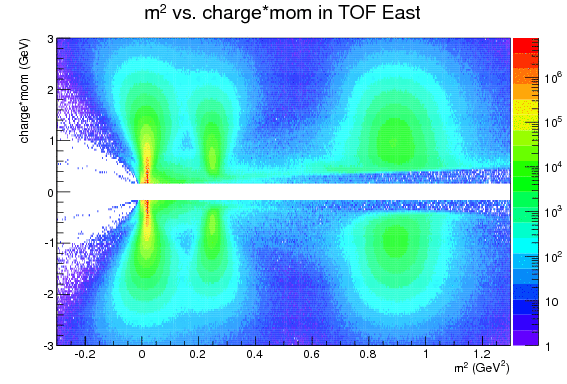
\includegraphics[scale=0.39]{pic/dat/nm/h_m2sum_tofe_all.png}
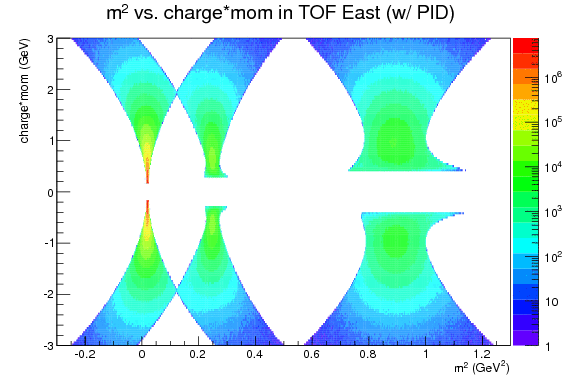
\includegraphics[scale=0.39]{pic/dat/nm/h_m2sum_tofe_pid.png}\\
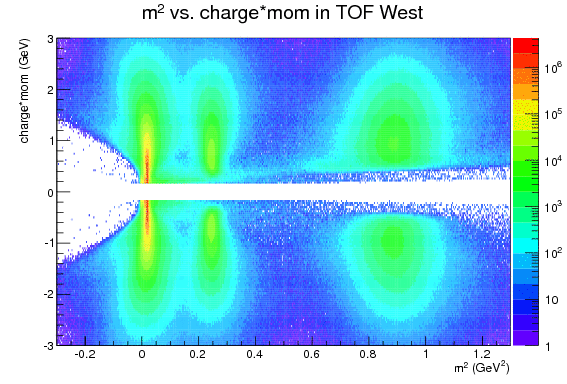
\includegraphics[scale=0.39]{pic/dat/nm/h_m2sum_tofw_all.png}
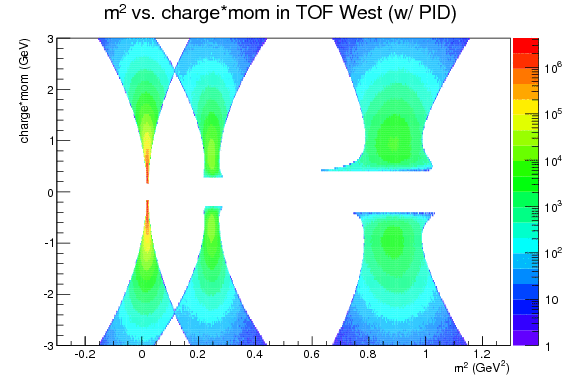
\includegraphics[scale=0.39]{pic/dat/nm/h_m2sum_tofw_pid.png}
%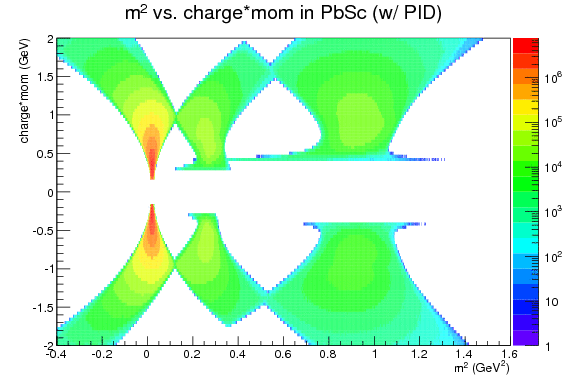
\includegraphics[scale=0.39]{pic/dat/nm/h_m2sum_pbsc_pid.png}
\caption{Nagy Márton által végzett részecskeazonosítás a TOF detektorokban, $2\sigma$ PID vágások alkalmazása mellett (baloldali ábra vágás nélkül, jobb oldali a PID vágás alkalmazása után).}
\label{fig:m2sum1}
\end{figure}

\begin{figure}[H]
\centering
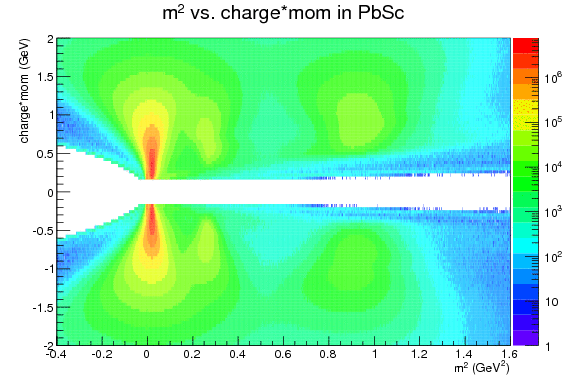
\includegraphics[scale=0.39]{pic/dat/nm/h_m2sum_pbsc_all.png}
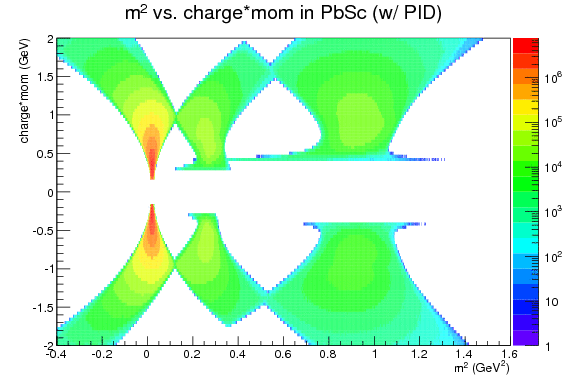
\includegraphics[scale=0.39]{pic/dat/nm/h_m2sum_pbsc_pid.png}
%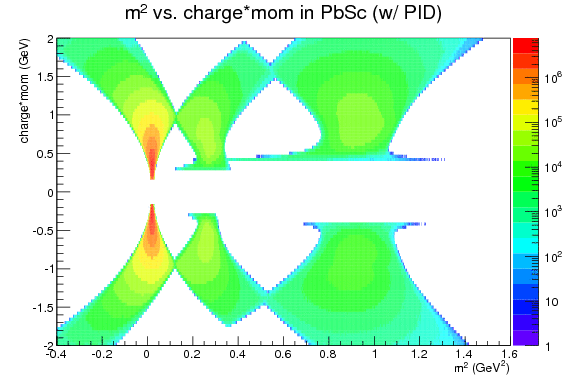
\includegraphics[scale=0.39]{pic/dat/nm/h_m2sum_pbsc_pid.png}
\caption{Nagy Márton által végzett részecskeazonosítás a PbSc detektorokban, $2\sigma$ vágások alkalmazása mellett (baloldali ábra vágás nélkül, jobb oldali a PID vágás alkalmazása után).}
\label{fig:m2sum1}
\end{figure}

\subsection{Kétrészecske vágások}

Ettől a fejezettől kezdve a PbSc detektorok keleti karban levő részére EMCE, a nyugati karban levő részére pedig EMCW rövidítésekkel hivatkozok. Továbbá a Drift Chamber (DC) detektor nevét olykor DCH rövidítéssel írom.

A korrelációs függvény mérésekor figyelembe kell venni a különböző detektorok pontatlanságát, amely a pálya rekonstrukciós algoritmus sajátosságaiból adódik. A pálya rekonstrukciója során két effektus okoz hibát: közeli részecskepályák esetén az algoritmus összeolvaszthatja a két részecskét eggyé valamint az is megtörténhet, hogy egy pályát ketté oszt az algoritmus, létrehozva egy úgynevezett ``szellem'' részecskét. Ezen effektusok kiküszöbölése érdekében kétrészecske vágásokat alkalmazunk, melynek során kidobjuk az adott távolságnál közelebb eső részecskéket. Ezen vágások megkonstruálása érdekében vizsgáltuk a kétrészecske pályatávolságok, a $\Delta z$ és $\Delta\varphi$, eloszlását a különböző detektorokban, amelyeket ~\aref{fig:paircuts} ábrák mutatnak különböző detektorban, az alkalmazott vágásokkal együtt (mivel ezen vágások is azonosak a kétrészecske analízis során alkalmazott vágásokkal ezért a bemutatott ábrák esztétikai okokból abból az analízisből származnak ~\cite{AN1244}).

A különböző detektorokban a kétrészecske vágásokat az alábbi egyenletekkel definiáltuk:

\begin{itemize}
\item DCH, EMCE, EMCW:
\begin{equation}
\Delta\varphi > \Delta\varphi_0-\frac{\Delta\varphi_0}{\Delta z_0}\Delta z \textnormal{ és } \Delta\varphi > \Delta\varphi_1 \label{e:newdchpaircut}
\end{equation}
\item TOFE:
\begin{equation}
\Delta\varphi > \Delta\varphi_0-\frac{\Delta\varphi_0}{\Delta z_0}\Delta z \label{e:newtofepaircut}
\end{equation}
\item TOFW:
\begin{equation}
\Delta\varphi > \Delta\varphi_0 \textnormal{ és } \Delta z > \Delta z_0 \label{e:newtofwpaircut}
\end{equation}
\end{itemize}

Az egyenletekben megjelenő paramétereket ~\aref{tab:paircuts} táblázat foglalja össze. A végső számolás során a $0$ sorszámú vágást alkalmaztam, a táblázatban szereplő többi értéket a szisztematikus hiba analízis során használtam.

\begin{table}[H]
\begin{center}
\begin{tabular}{|c||c|c|c||c|c|c||c|c||c|c|}\hline
\multirow{2}{*}{\small{vágás}} 
& \multicolumn{3}{c||}{DCH}
& \multicolumn{3}{c||}{EMC}
& \multicolumn{2}{c||}{TOFE}
& \multicolumn{2}{c|}{TOFW}\\
  & $\Delta z_0$ [fm] & $\Delta \varphi_0$ & $\Delta \varphi_1$ 
  & $\Delta z_0$ [fm] & $\Delta \varphi_0$ & $\Delta \varphi_1$
  & $\Delta z_0$ [fm] & $\Delta \varphi_0$
  & $\Delta z_0$ [fm] & $\Delta \varphi_0$\\\hline\hline
0 & 11 & 0.15 & 0.025 & 18 & 0.14 & 0.020 & 13 & 0.13 & 15.0 & 0.14\\\hline
1 & 10 & 0.14 & 0.020 & 18 & 0.14 & 0.020 & 13 & 0.13 & 15.0 & 0.14\\\hline
2 & 12 & 0.16 & 0.030 & 18 & 0.14 & 0.020 & 13 & 0.13 & 15.0 & 0.14\\\hline
3 & 11 & 0.15 & 0.025 & 17 & 0.13 & 0.015 & 12 & 0.12 & 14.5 & 0.13\\\hline
4 & 11 & 0.15 & 0.025 & 19 & 0.15 & 0.025 & 14 & 0.14 & 15.5 & 0.15\\\hline

\end{tabular}
\end{center}
\caption{A (\ref{e:newdchpaircut})-(\ref{e:newtofwpaircut}) egyenletekben használt vágások paraméterei. A vágások hatását függetlenül vizsgáljuk, a 0-2 vágások a DCH detektorra, a 0,3,4 vágások pedig az EMC, TOFE, TOFW detektorokra vonatkoznak.}
\label{tab:paircuts}
\end{table}

\begin{figure}[H]
\centering
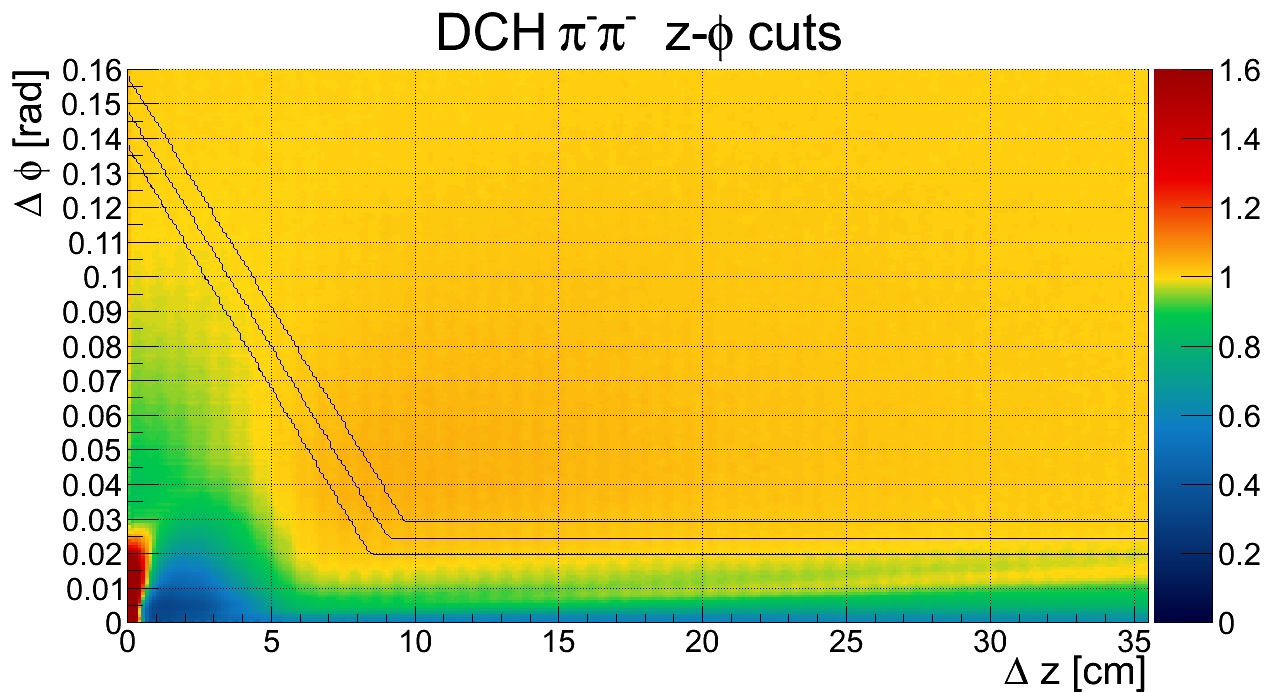
\includegraphics[scale=0.17]{pic/dat/kd/Corr_DCH_dzdp_mm.png}
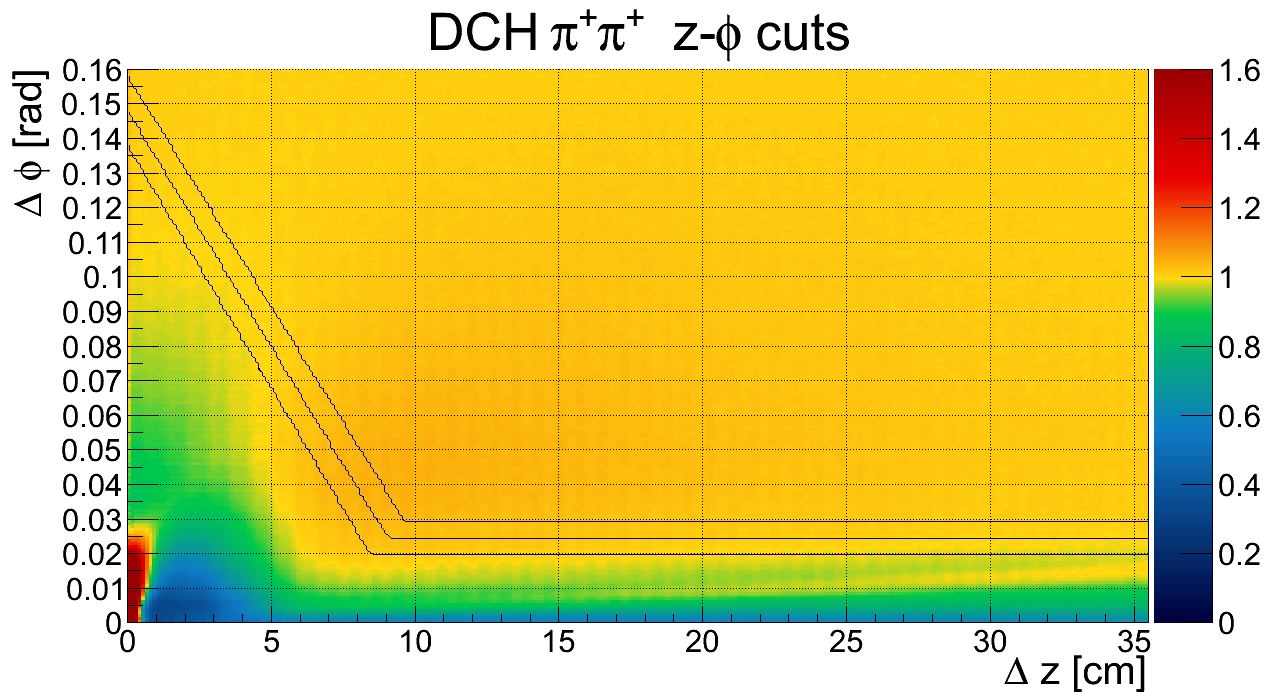
\includegraphics[scale=0.17]{pic/dat/kd/Corr_DCH_dzdp_pp.png}\\
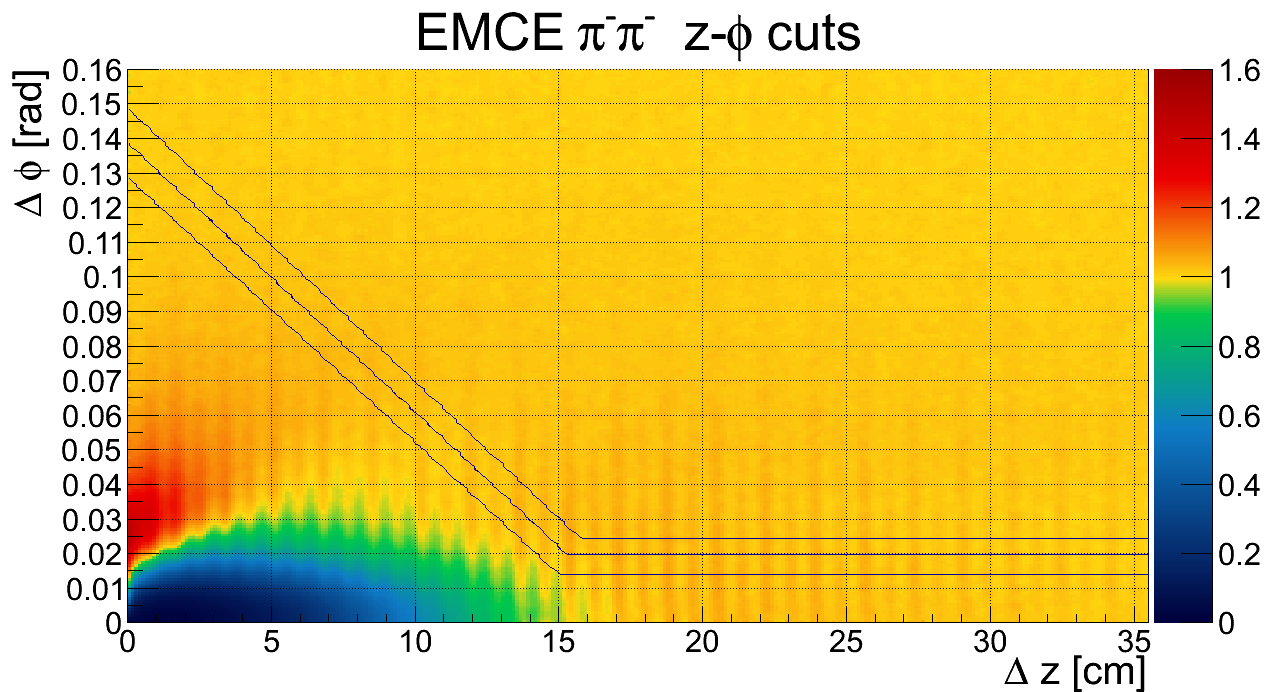
\includegraphics[scale=0.17]{pic/dat/kd/Corr_EMCE_dzdp_mm.png}
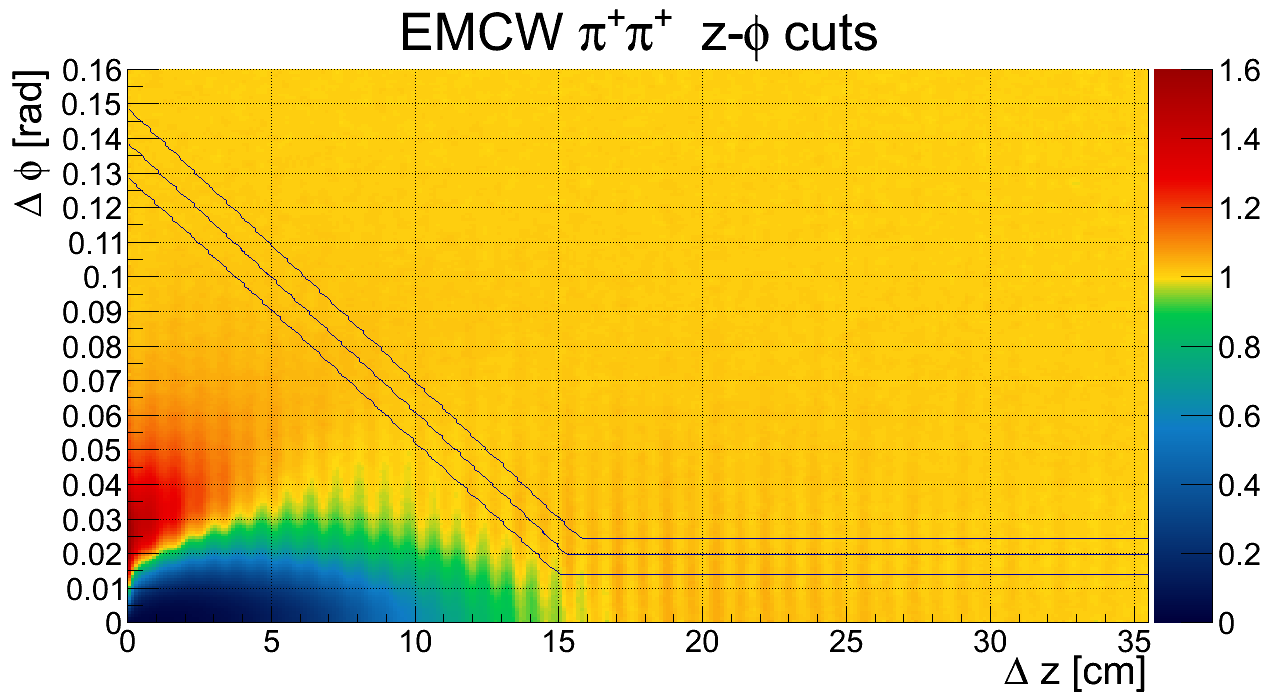
\includegraphics[scale=0.17]{pic/dat/kd/Corr_EMCW_dzdp_pp.png}\\
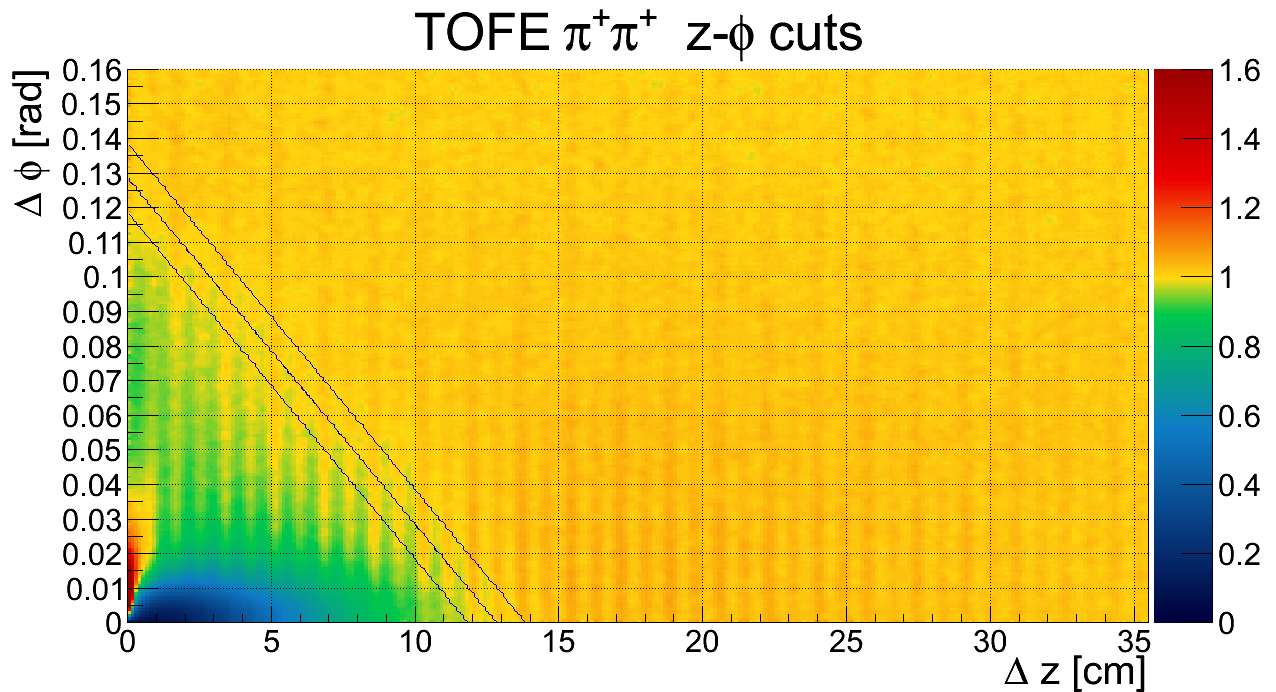
\includegraphics[scale=0.17]{pic/dat/kd/Corr_TOFE_dzdp_pp.png}
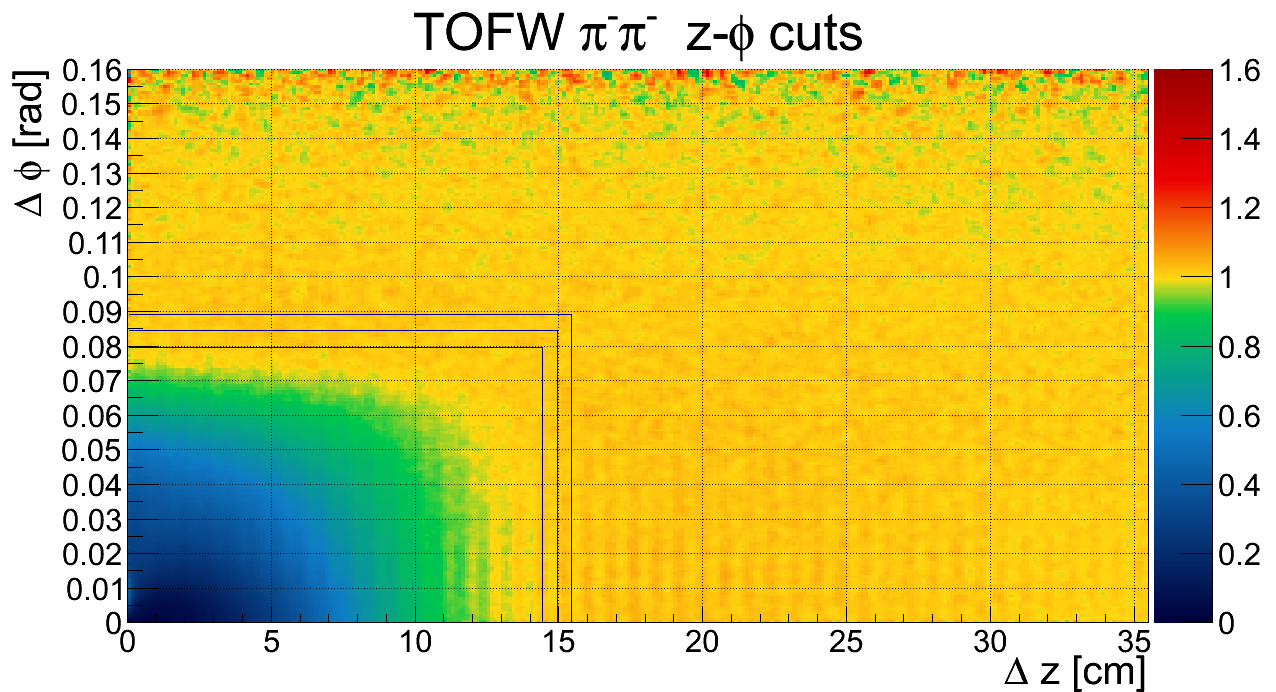
\includegraphics[scale=0.17]{pic/dat/kd/Corr_TOFW_dzdp_mm.png}
\caption{A kétrészecske analízis során készült $\Delta\varphi-\Delta z$ eloszlások, és az alkalmazott vágások a különböző detektorokban.}
\label{fig:paircuts}
\end{figure}


\subsection{Korrelációs függvény változói}

~\Aref{sec:C20} fejezetben láttuk, hogy a kétrészecske korrelációs függvényben célszerű áttérni a $2k=p_1-p_2$ és $2K=p_1+p_2$ változókra. A korrelációs függvény  $K$ függése tipikusan simább mint a $k$ függés ~\cite{Lisa:2005dd}, ekkor szokás alkalmazni a $p_1\approx p_2\approx K$ közelítést, azaz feltesszük, hogy a $K$ körülbelül tömeghéjon van. Ennek következtében ~\aref{eq:kK} egyenlet kihasználásával a kétrészecske korrelációs függvény vizsgálható a $\bm{k}$ és $\bm{K}$ hármas vektorok függvényeként, ahol a $\bm{k}$-ra gondolhatunk fő kinematikai változóként. Továbbá midrapiditáshoz közel a $\bm{K}$ hármasvektor helyett áttérhetünk $K_T$ (transzverz momentum nagysága) vagy $m_T$ (transzverz tömeg) változókra, amelyeket a következő összefüggések definiálnak:
\begin{equation}
K_T = \frac{1}{2}\sqrt{K_x^2+K_y^2},\;\;\;\;\;\;\;\;
m_Tc = \sqrt{m^2c^2+K_T^2},
\end{equation}
ahol $m$ a piontömeg és $\bm{K}=(K_x, K_y, K_z)$.

Háromrészecske korrelációk vizsgálata során szintén áttérünk a már bevezetett $2k_{ij}=p_i-p_j$ és  $3K=p_1+p_2+p_3$ változókra. Az előbb tárgyal tömeghéj közelítést ebben az esetben is megtehetjük ($p_1\approx p_2\approx p_3 \approx K$), melynek eredményeként áttérhetünk a $\bm{k}_{ij}$ és $\bm{K}$ hármasvektorokra, továbbá a $\bm{K}$ vektor helyett használhatjuk a $K_T$ (vagy $m_T$) skalár változót.

Tehát különböző $m_T$ tömegek esetén mérjük a háromrészecske korrelációs függvényt, mint a $\bm{k}_{ij}$ változók függvénye. A relatív momentumok esetén használjuk a  Bertsch-Pratt (BP) ~\cite{Pratt:1986ev,Bertsch:1988db} dekompozíciót, melynek keretében a vektort out-side-long irányokra bontjuk, ahol az out az átlagos transzverz momentum iránya, a long a nyalábirány, a side pedig az előző kettőre merőleges:
\begin{equation}
\bm{k}_{ij} = (k_{ij}^{\mathrm{out}}, k_{ij}^{\mathrm{side}}, k_{ij}^{\mathrm{long}})
\end{equation}
 Szokás még áttérni a longitudinálisan együtt mozgó rendszerre (LCMS) egy longitudinális irányba végzett Lorentz boost segítségével ~\cite{Wiedemann:1999qn}.

Tehát ezek alapján a háromrészecske korrelációs függvény a $\bm{k}_{ij}^{\mathrm{LCMS}}$ vektorok és $m_T$ függvénye, azaz minden $m_T$ esetén egy $6$ dimenziós eloszlás. Mivel nincsen elég adat ilyen magas dimenzióban a korrelációs függvény meghatározásához, ezért $\bm{k}_{ij}^{\mathrm{LCMS}}$ vektorokról át kell térnünk valamilyen skalár mennyiségekre, így csökkentve a dimenziószámot háromra. Kétrészecske korrelációk vizsgálata során is gyakran áttérnek a $3$ dimenziós relatív momentum vektorról valamilyen skalár mennyiségre, így növelve a statisztikát ~\cite{Achard:2011zza, Khachatryan:2011hi}. Kétrészecske esetén a legegyszerűbb Lorentz-transzformációra invariáns mennyiséget a következőképpen kapjuk:
\begin{equation}
k_{\mathrm{inv}} = \sqrt{k_\mu k^\mu} = \sqrt{(1-\beta_T)^2k_{\mathrm{out}}^2+k_{\mathrm{side}}^2+k_{\mathrm{long}}^2},
\end{equation}
ahol $\beta_T=\frac{2K_T}{E_1+E_2}$. Az összefüggés mutatja, hogy $k_{\mathrm{inv}}$ értéke lehet kicsi, miközben a $k_{\mathrm{out}}$ nagy, ha a $\beta_T$ $1$-hez közeli.

A Bose-Einstein korrelációk korábbi vizsgálata során kiderült, hogy $\sqrt{s_{NN}}=200\;\mathrm{GeV}$ tömegközépponti energián végzett ütközések esetén az úgynevezett Bertsch-Pratt-sugarak ($R_\mathrm{out}$, $R_\mathrm{side}$, $R_\mathrm{long}$) azonos nagyságrendűek, azaz a korrelációs függvény közel gömbszimmetrikus az LCMS rendszerben ~\cite{Adler:2004rq, Afanasiev:2009ii, Adams:2004yc, Afanasiev:2007kk}. Amennyiben az LCMS rendszer helyett a pár tömegközépponti rendszerébe (PCMS) térünk át, teljesülni fog, hogy:
\begin{equation}
k_{\mathrm{inv}}=\abs{\bm{k}^{\mathrm{PCMS}}}
\end{equation}
Ebben a rendszerben azonban a korrelációs függvény már nem lesz gömbszimmetrikus, így $\sqrt{s_{NN}}=200\;\mathrm{GeV}$ tömegközépponti energián a $k_{\mathrm{inv}}$ nem jó választás. Ezért egy olyan változóra kell áttérnünk, amelynek kis értékei esetén teljesül, hogy mindhárom komponens értéke kicsi. A legegyszerűbb ilyen választás az LCMS rendszerben a momentumkülönbség vektor nagysága (jel. $k=\bm{k_{\mathrm{LCMS}}}$). A $k$ a laborrendszerben vett változók segítségével a következő lesz:
\begin{equation}
k=\sqrt{k_x^2+k_y^2+k_{\mathrm{long,LCMS}}^2},
\end{equation} 
ahol $2k_{x/y}=p_{1,x/y}-p_{2,x/y}$ és
\begin{equation}
k_{\mathrm{long,LCMS}}^2=\frac{(p_{1z}E_2-p_{2z}E_1)^2}{(E_1+E_2)^2-(p_{1z}-p_{2z})^2}
\end{equation}

A kétrészecske esetén látottak alapján a háromrészecske korrelációk vizsgálata során, a kétrészecske momentumkülönbség vektorok helyett az LCMS koordináta-rendszerben számolt nagyságukra térünk át. Így laborrendszerben mért változók segítségével a korrelációs függvény változói a következőképpen számolhatók:
\begin{equation}
k_{ij} = \abs{\bm{k}^{\mathrm{LCMS}}_{ij}} = \sqrt{k_{ij, x}^2+k_{ij, y}^2+k_{ij, \mathrm{long, LCMS}}^2},
\end{equation}
ahol
\begin{equation}
k_{ij, \mathrm{long, LCMS}}^2 = \frac{
\Big[p_{iz}E_j-p_{jz}E_i+\frac{1}{2}E_k(p_{iz}-p_{jz})-\frac{1}{2}(E_i-E_j)p_{kz}\Big]^2
}{(E_1+E_2+E_3)^2-(p_{1z}+p_{2z}+p_{3z})^2},
\end{equation}
ahol $i\neq j\neq k$.

Tehát a korrelációs függvényt különböző $m_T$ esetén a $k_{ij}$ LCMS rendszerben vett momentumkülönbség nagyságok függvényében vizsgáljuk, így a dimenziószámot $6$-ról $3$-ra redukáltuk.
 
\subsection{Korrelációs függvény mérése}

A korrelációs függvény mérése során az adott eseményben beazonosított részkecskénekből tripletteket képezünk. Ezután a triplettben a részecskepárok momentum különbségéből az előző fejezetben tárgyalt módon meghatározzuk nagyságukat a longitudinálisan együtt mozgó rendszerben. Ezen nagyságokból elkészítünk egy 3 dimenziós momentum eloszlást a triplettek transzverz tömegeinek különböző értékeire (transzverz tömegek tartományát összesen 32 bin-re osztottuk). Ideális esetben ez lenne a korrelációs függvény, azonban ezen mérési módszer során azonban nem vettük figyelembe a detektorok jelentős kinematikai akceptanciai effektusait. Ezen effektusok kiküszöbölése érdekében az úgynevezett eseménykeverés módszerét kell alkalmazni.

Az eseménykeverés módszere során az ideális esetben korrelációs függvényt megadó eloszlást aktuális eloszlásnak nevezzük, és $\mathcal{A}(k_{12},k_{23},k_{31})$ jelölést alkalmazzuk rá (ez az eloszlás az ideálistól jelentősen eltér). Az aktuális eloszlás mellett meg kell határoznunk egy háttéreloszlást ($\mathcal{B}(k_{12},k_{23},k_{31})$), amelyet az $\mathcal{A}$ eloszláshoz hasonló módon, azonban a triplett tagjait különböző eseményből véve kapunk, így ez csupán a detektorok által mesterségesen létrehozott korrelációt tartalmazza. Ezen eloszlás segítségével már megkapható a korrelációs függvény:
\begin{equation}
C_3(k_{12},k_{23},k_{31}) = \frac{\mathcal{A}(k_{12},k_{23},k_{31})}{\mathcal{B}(k_{12},k_{23},k_{31})}\frac{\int \mathcal{B}(k_1, k_2, k_3) dk_1dk_2dk_3}{\int \mathcal{A}(k_1,k_2,k_3)dk_1dk_2dk_3},
\end{equation}
ahol az integrálás olyan tartományon történik ahol a korrelációs függvény már nem mutat kvantumstatisztikai effektusokat.

Ahhoz, hogy biztosítsuk, hogy a háttéreloszlás a hasonló kinematikai akceptancia effektusokat tartalmazza, teljesülnie kell, hogy az aktuális és háttéresemények hasonlóak $z-$vertex pozícióban és centralitásban. Ezért a $z-$vertex tartományát $2$ cm, a centralitási tartományt pedig $3\%$ felbontással felosztottam, és az aktuális eseményhez az azonos centralitás és $z-$vertex bin-ben levő háttéreseményeket választottam.

Az eseménykeverés módszere során a háttéreloszlás meghatározása többféleképpen történhet. Az általam alkalmazott eseménykeverő módszert ~\aref{fig:mixingevents} ábra szemlélteti. A módszer során az eseményekből egy $N_\mathrm{pool}$ méretű háttérhalmazt készítünk, amelynek mérete legalább akkora mint a legnagyobb esemény multiplicitása. Az aktuális eloszlás meghatározása során, az esemény minden pionjához véletlenszerűen választunk egy eseményt a háttérhalmazból, majd a választott eseményből sorsolunk egy az aktuális eseményből származó pion töltésével egyező piont. Az így kapott háttérrészecskékből az $\mathcal{A}$ eloszláshoz hasonlóan meghatározzuk a $\mathcal{B}$ háttéreloszlást. 


\begin{figure}[H]
\centering
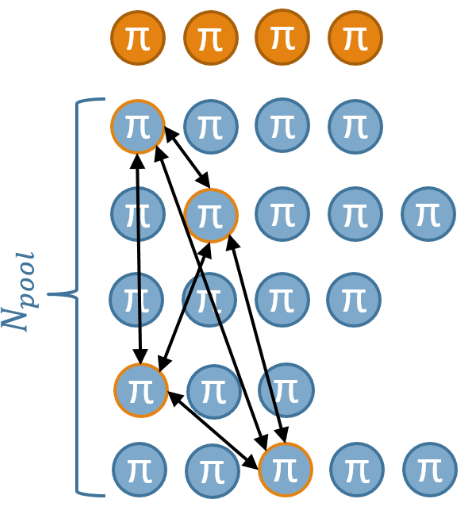
\includegraphics[scale=0.5]{pic/dat/mixingevents}
\caption{A használt eseménykeverő módszer szemléltetése: az aktuális esemény multiplicitásával megegyező számú régi eseményt választunk véletlenszerűen, majd minden eseményből egy részecskét sorsolunk.}
\label{fig:mixingevents}
\end{figure}


Az aktuális és háttéreloszlások meghatározása során, kitüntetek egy sorrendet a triplettek részecskéi között, mivel így sokkal hatékonyabb az eloszlásokat meghatározó algoritmus. Azonban fizikailag a sorrend nem számít, ezért fontos ezen mesterséges effektustól való megszabadulás. Ezt a $\mathcal{A},\; \mathcal{B}$ eloszlások összehajtogatásával tehetjük meg.  Ez azt jelenti, hogy, ha az aktuális eloszlás $(i,j,k)$ bin-ben levő értékéhez, hozzá kell adnunk az indexek minden lehetséges permutációját (lenullázva ezeket), azaz:
\begin{equation}
\mathcal{A}(i, j, k) = \mathcal{A}(i,j,k) + \mathcal{A}(i, k, j) + \mathcal{A}(k, i, j) + \mathcal{A}(k, j, i) + \mathcal{A}(j, k, i) + \mathcal{A}(j, i, k).
\end{equation}
A hajtogatást az aktuális és háttéreloszláson kell végezni, a korrelációs függvény meghatározása előtt. ~\Aref{fig:f4} ábra mutatja az aktuális eloszlást hajtogatás előtt és után. Az ábrákon látjuk továbbá, hogy a $\vec{k}_{12}$, $\vec{k}_{13}$, $\vec{k}_{23}$ között teljesül a háromszög-egyenlőtlenség.

\begin{figure}[H]
\centering
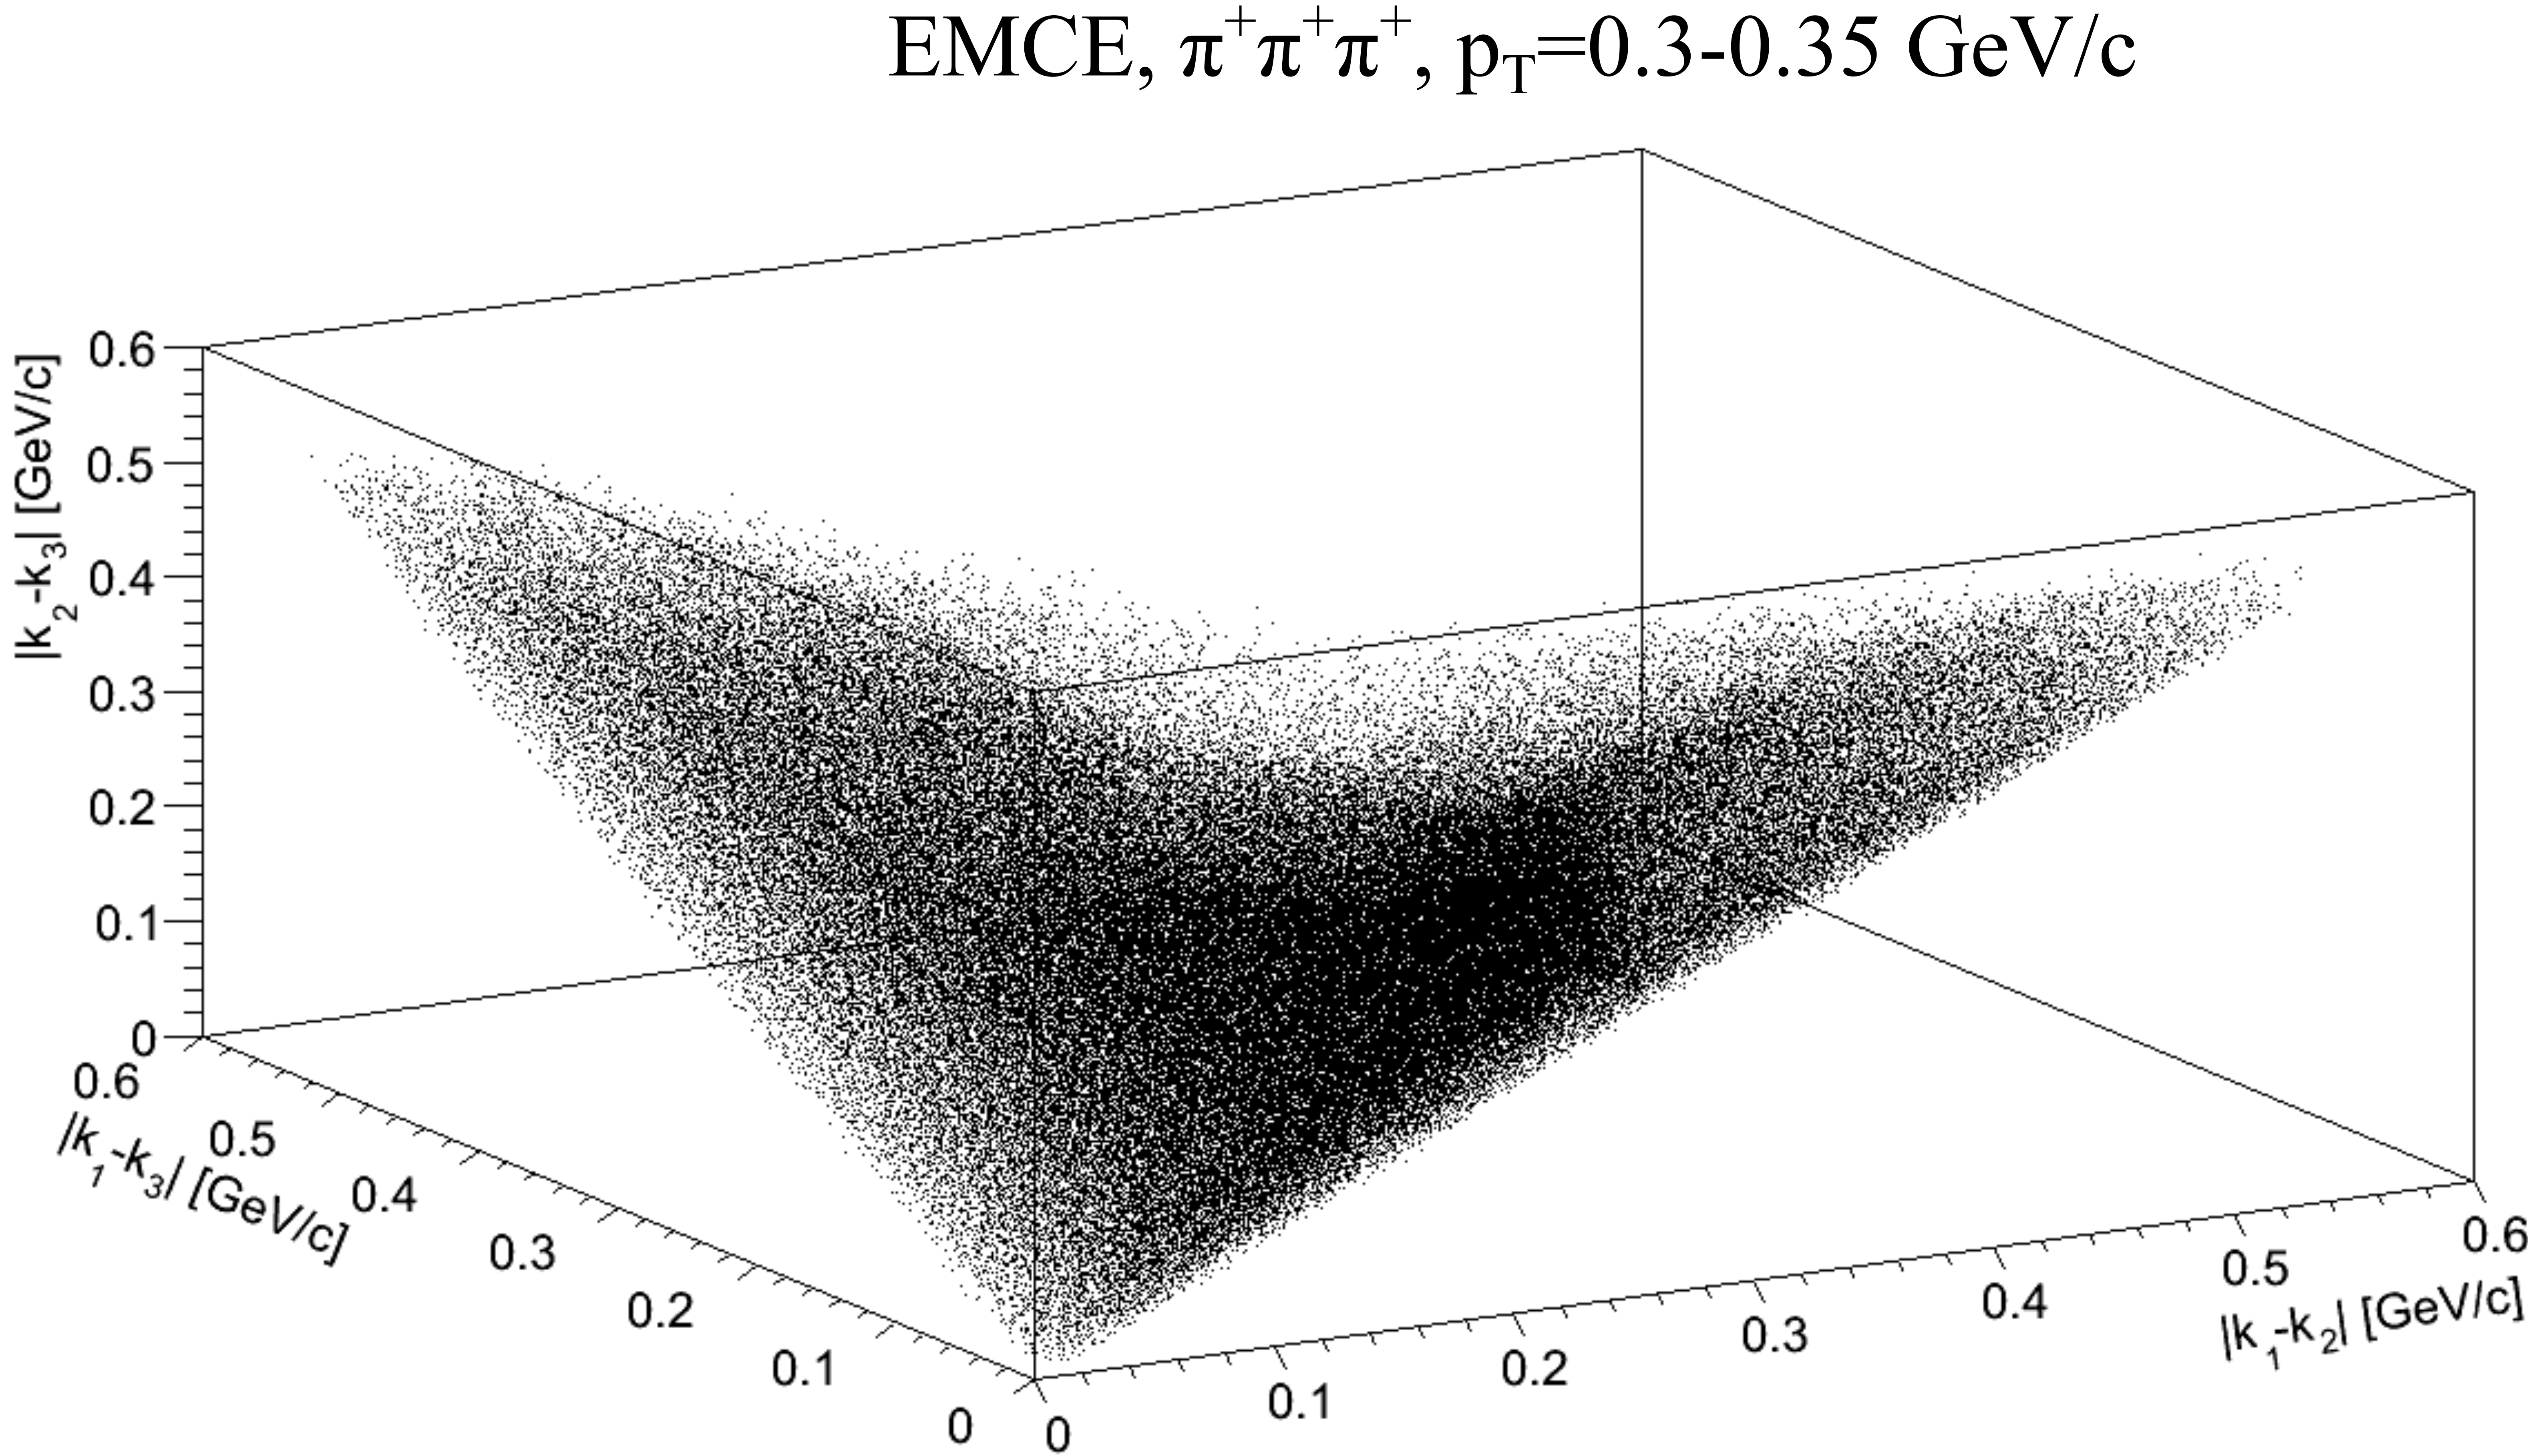
\includegraphics[scale=0.24]{pic/corrfunc/C1}
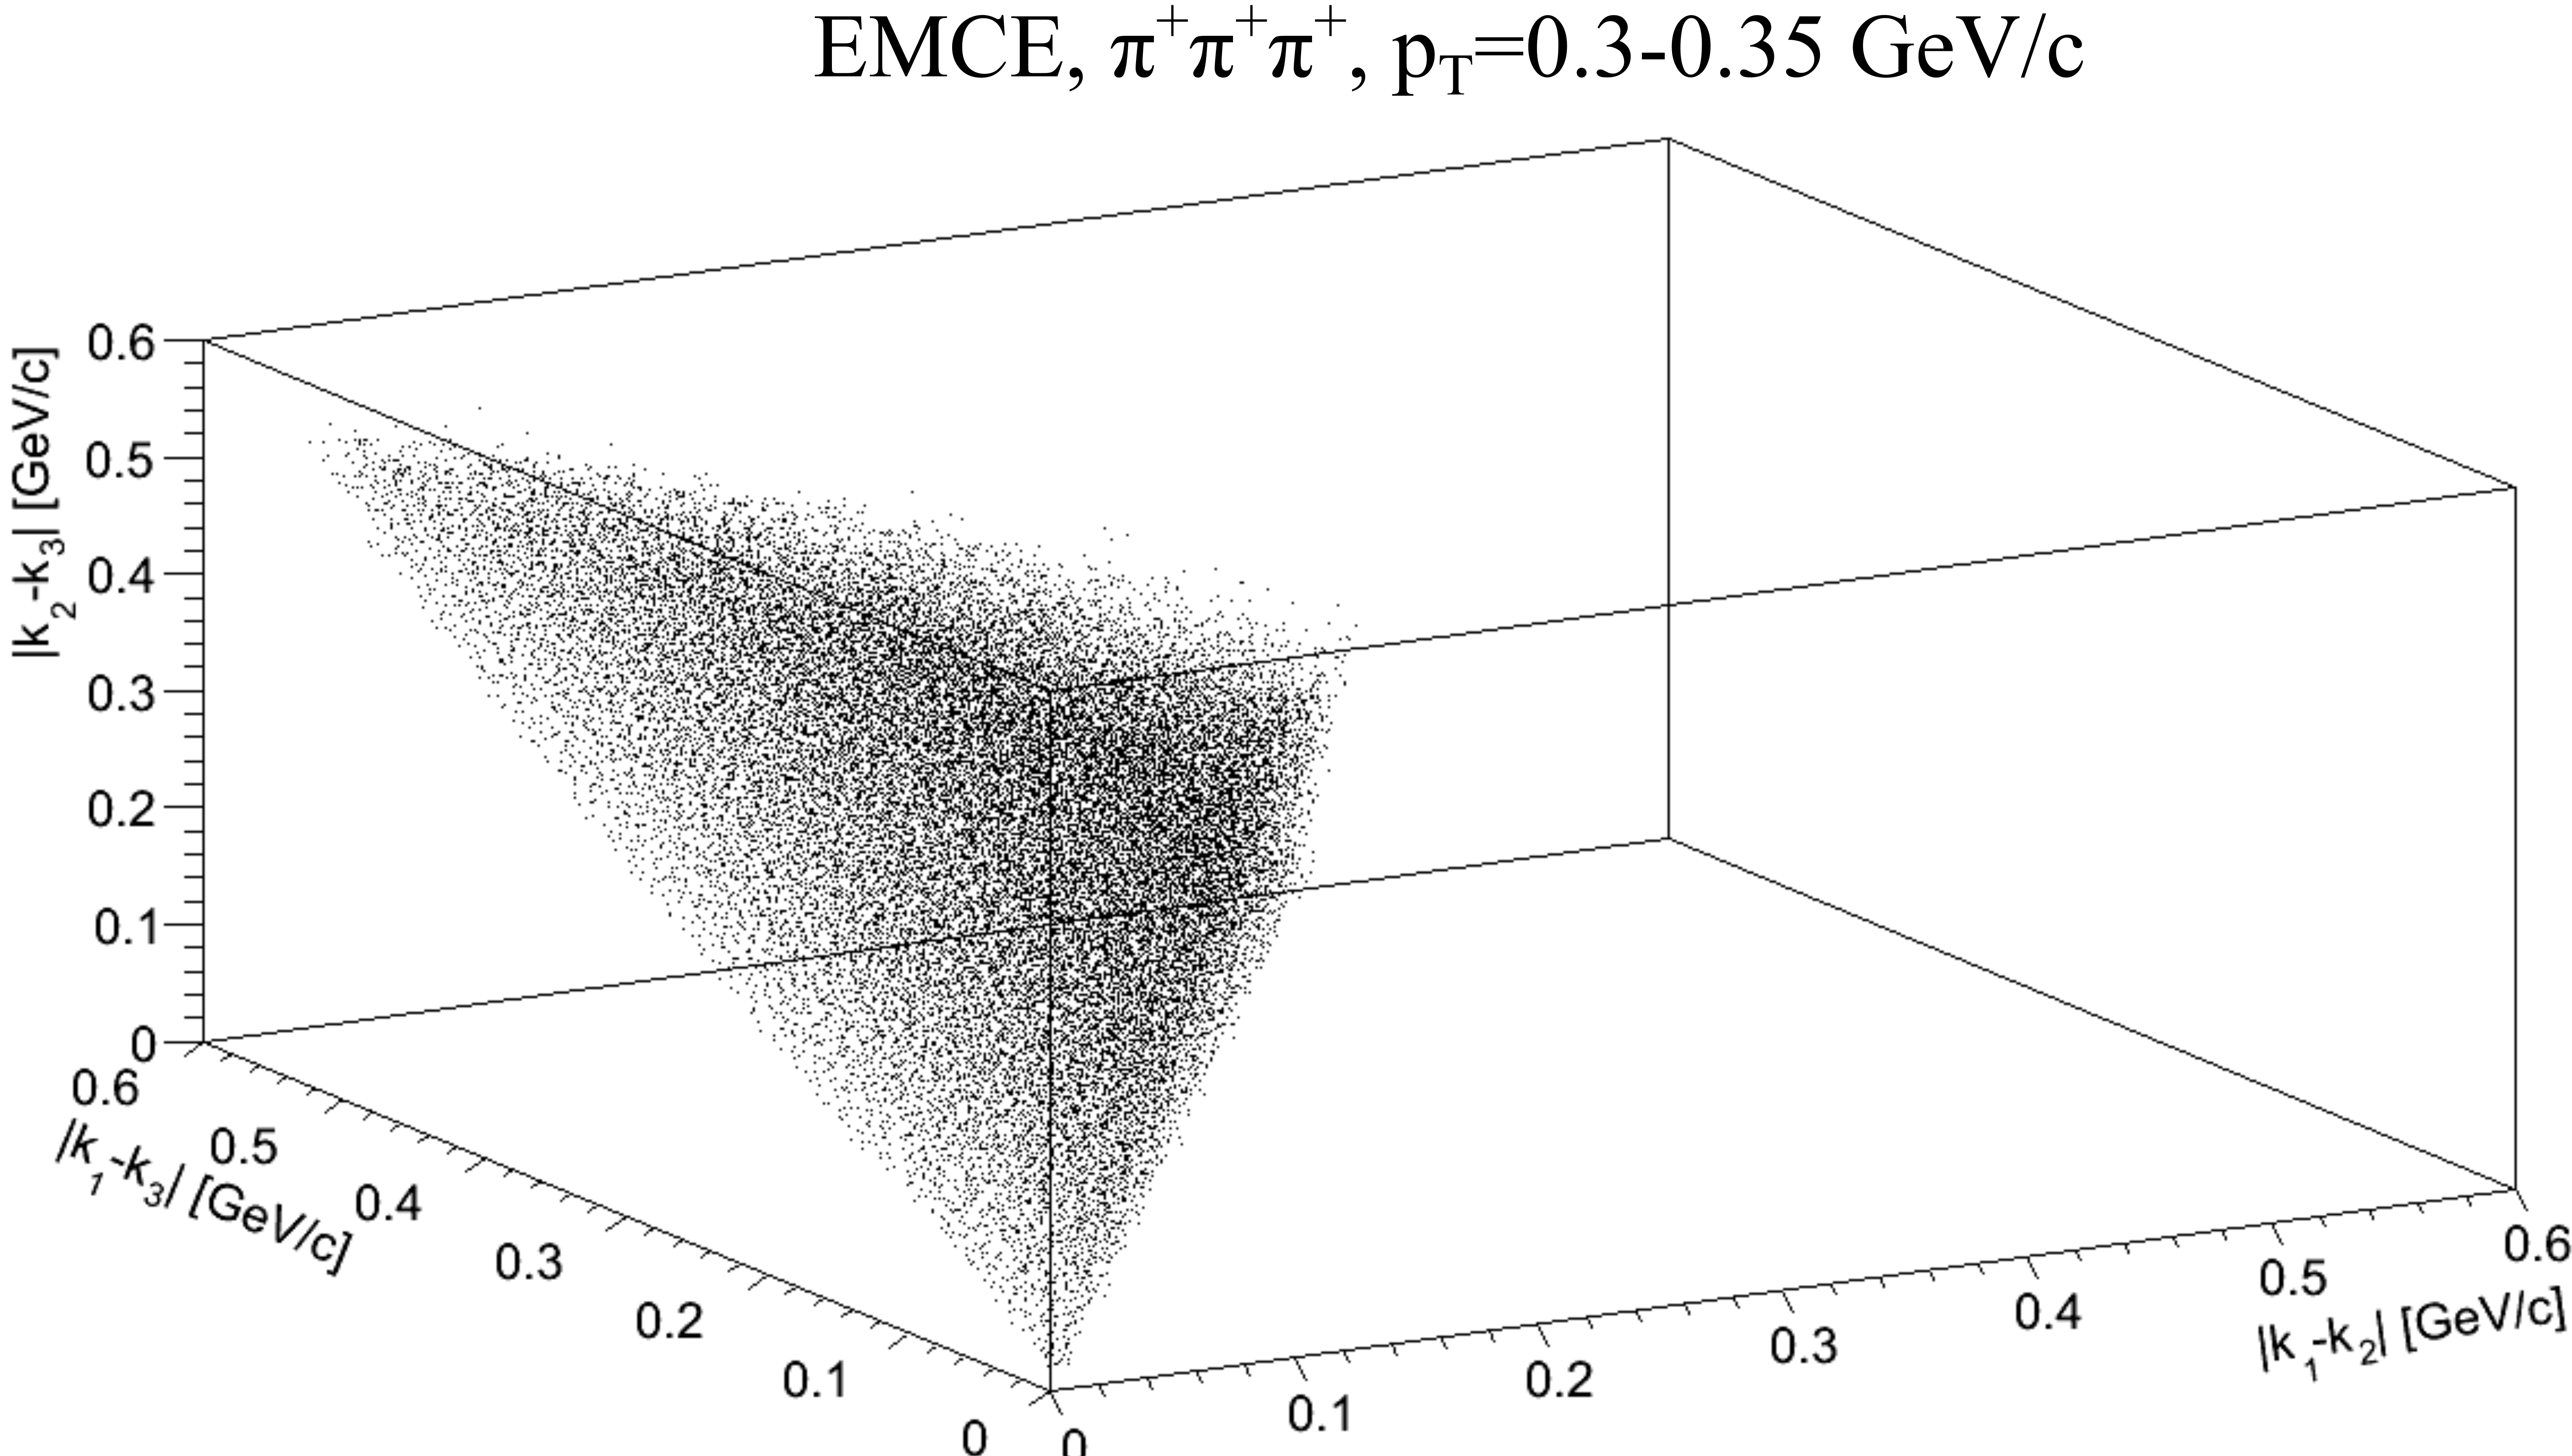
\includegraphics[scale=0.24]{pic/corrfunc/C2}
\caption{Baloldali ábra mutatja a mérés utáni (hajtogatás előtti) aktuális eloszlást, míg a jobboldali a hajtogatás utáni eloszlást.}
\label{fig:f4}
\end{figure}


\subsection{Illesztett modell}\label{sec:fit}

A kvantumstatisztikai modell meghatározása a kétrészecskés esetben bemutatotthoz hasonlóan történik, azaz kétrészecskés hullámfüggvény relatív koordinátafüggésére síkhullámot használunk:
\begin{equation}
\Psi_{\boldsymbol{k_{ij}}}(\boldsymbol{r_{kl}})=e^{i\boldsymbol{k_{ij}}\boldsymbol{r_{kl}}},
\end{equation}
majd három ilyen hullámfüggvény szorzatának szimmetrizálása után kapjuk meg a háromrészecske hullámfüggvényt:
\begin{align}
\begin{split}
\Psi_{\boldsymbol{k_{12}},\boldsymbol{k_{23}},\boldsymbol{k_{31}}}(\boldsymbol{r_{12}},\boldsymbol{r_{23}},\boldsymbol{r_{31}})=&\frac{1}{\sqrt{6}}\Big(e^{i\boldsymbol{\frac{2}{3}k_{12}}\boldsymbol{r_{12}}}e^{i\frac{2}{3}\boldsymbol{k_{23}}\boldsymbol{r_{23}}}
e^{i\frac{2}{3}\boldsymbol{k_{31}}\boldsymbol{r_{31}}}+
e^{i\frac{2}{3}\boldsymbol{k_{12}}\boldsymbol{r_{13}}}e^{i\frac{2}{3}\boldsymbol{k_{23}}\boldsymbol{r_{32}}}
e^{i\frac{2}{3}\boldsymbol{k_{31}}\boldsymbol{r_{21}}}+\\
+&e^{i\frac{2}{3}\boldsymbol{k_{12}}\boldsymbol{r_{21}}}e^{i\frac{2}{3}\boldsymbol{k_{23}}\boldsymbol{r_{13}}}
e^{i\frac{2}{3}\boldsymbol{k_{31}}\boldsymbol{r_{32}}}+
e^{i\frac{2}{3}\boldsymbol{k_{12}}\boldsymbol{r_{23}}}e^{i\frac{2}{3}\boldsymbol{k_{23}}\boldsymbol{r_{31}}}
e^{i\frac{2}{3}\boldsymbol{k_{31}}\boldsymbol{r_{12}}}+\\
+&e^{i\frac{2}{3}\boldsymbol{k_{12}}\boldsymbol{r_{31}}}e^{i\frac{2}{3}\boldsymbol{k_{23}}\boldsymbol{r_{12}}}
e^{i\frac{2}{3}\boldsymbol{k_{31}}\boldsymbol{r_{23}}}+
e^{i\frac{2}{3}\boldsymbol{k_{12}}\boldsymbol{r_{32}}}e^{i\frac{2}{3}\boldsymbol{k_{23}}\boldsymbol{r_{21}}}
e^{i\frac{2}{3}\boldsymbol{k_{31}}\boldsymbol{r_{13}}}\Big)
\label{eq:psi3}
\end{split}
\end{align}

Ezen hullámfüggvény használva, valamint a forrásfüggvény leírására Lévy eloszlást feltételezve elvégezhető ~\aref{eq:Cn} összefüggés által definiált háromrészecske korrelációs függvény kiszámolása. Áttérve az előző fejezetben tárgyalt változókra, ez a következő alakú lesz:

\begin{align}
C_3^{(0)}(k_{12}, k_{13}, k_{23}) = 1+ \ell_3e^{-0.5(|2k_{12}R|^\alpha+|2k_{13}R|^\alpha+|2k_{23}R|^\alpha)}\nonumber\\
+\ell_2\bigg(e^{|2k_{12}R|^\alpha}+e^{|2k_{13}R|^\alpha}+e^{|2k_{23}R|^\alpha}\bigg),
\end{align}

ahol $\ell_2$ a kétrészecske szektor korrelációs erőssége, $\ell_3$ pedig a háromrészecske szektor korrelációs erőssége. Ezek mag-glória modell esetén $f_C$ függvények.

A háromrészecske korrelációs erősség ebben az esetben a következő adódik:
\begin{equation}
\lambda_3(m_T) \equiv \lim_{\substack{k_{12}\rightarrow 0\\ k_{23}\rightarrow 0\\ k_{31}\rightarrow 0}} C_3(k_{12},k_{23}, k_{31}, m_T) = \ell_3(m_T)-3\ell_2(m_T)
\end{equation}


Annak érdekében, hogy a modellt illeszthessük, még be kell vezetnünk egy hátteret. A háttér leírására a legegyszerűbb függvényt választottuk, amely három koordinátában ugyanazon meredekséggel leírt lineáris függvény szorzatából áll:
\begin{equation}
C_{3, \mathrm{fit}}^{(0)}(k_{12}, k_{13}, k_{23})= N(1+\epsilon k_{12})(1+\epsilon k_{13})(1+\epsilon k_{23})C_3^{(0)}(k_{12}, k_{13}, k_{23})
\end{equation}
Tapasztalataink azt mutatták, hogy ez a háttérválasztás megfelelő, és nem kell a különböző változókhoz különböző meredekséget társítani, ami kettővel több illesztési paramétert eredményezne. Az illesztést a $k_{12}=k_{23}=k_{31}$ altéren ~\aref{fig:fit} ábra mutatja két különböző $m_T$ érték esetén. Az ábrán látszik, hogy az illesztések kellően pontosak.

\begin{figure}[H]
\centering
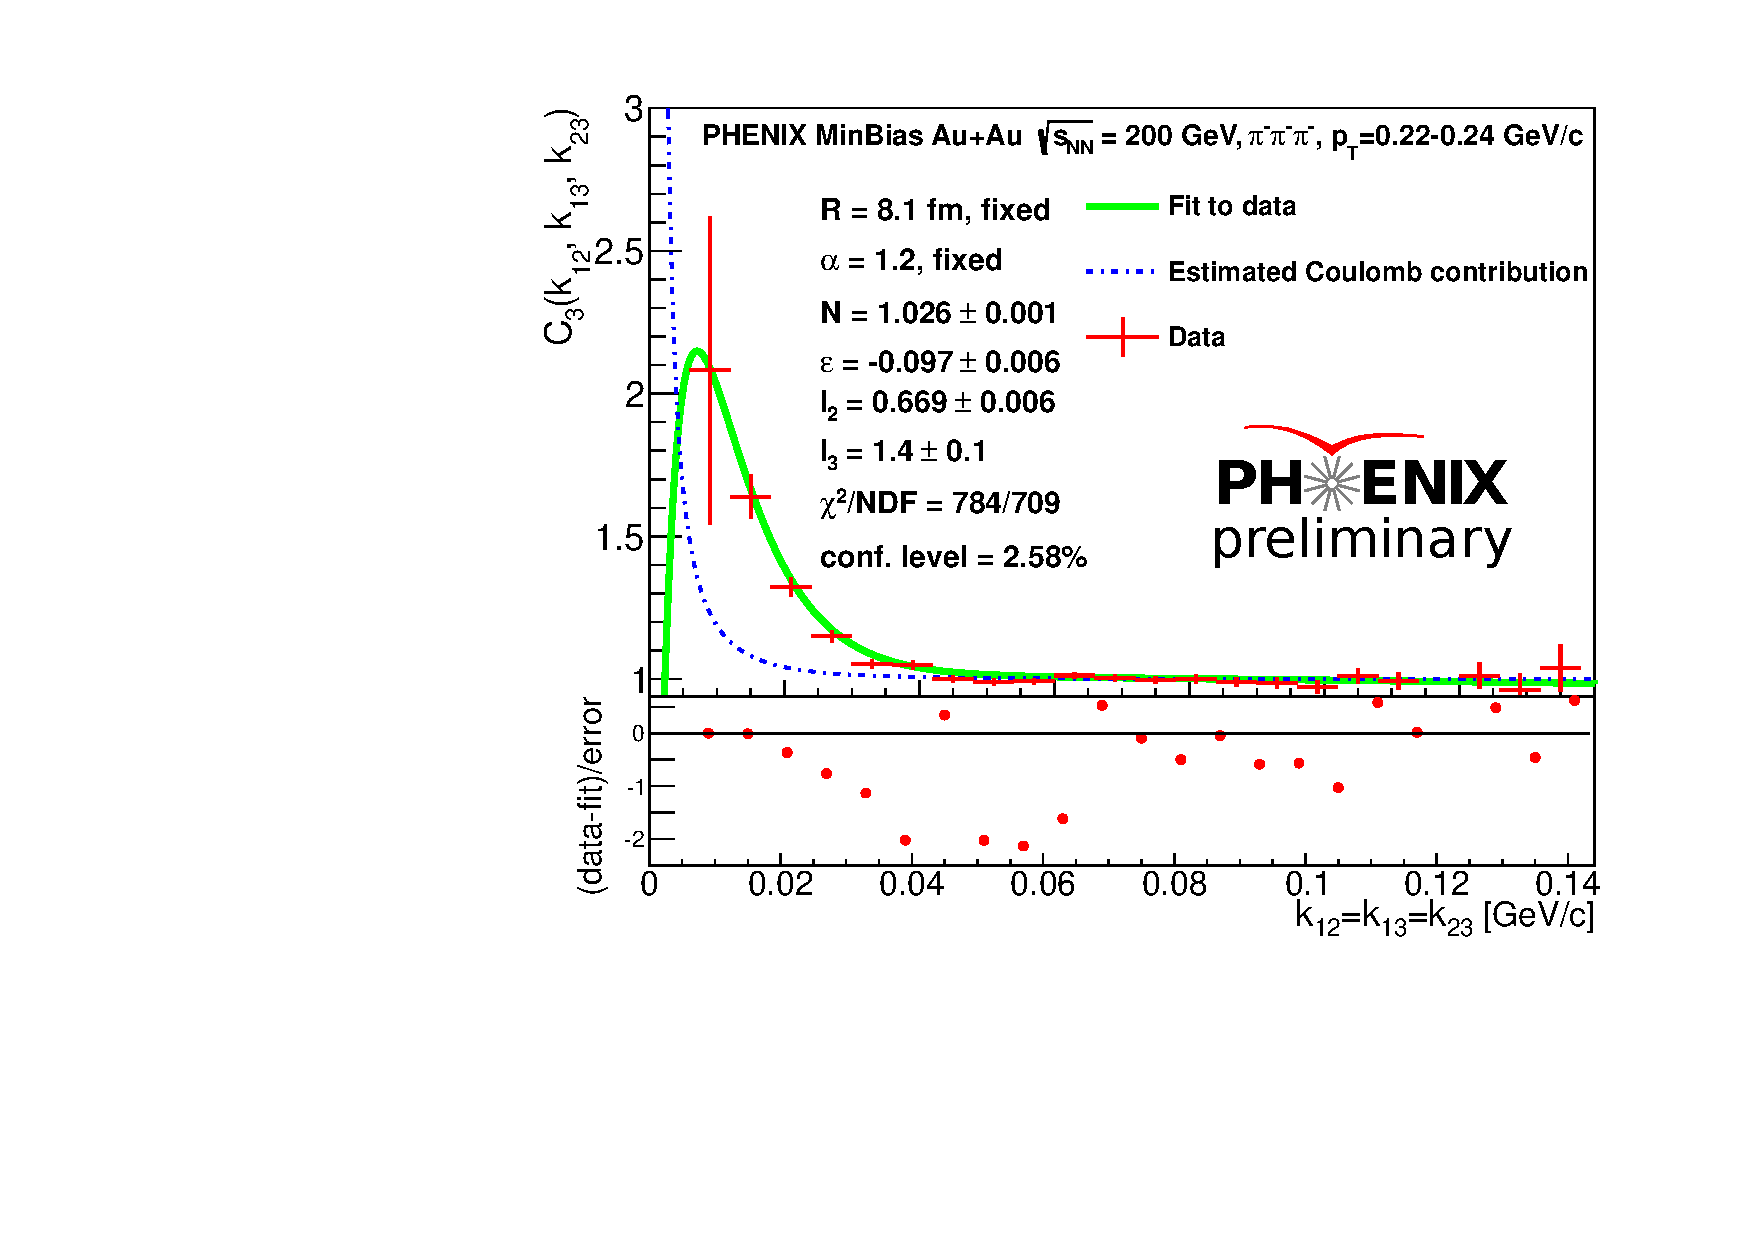
\includegraphics[scale=0.6]{pic/res/diag_lowpt.pdf}
\centering
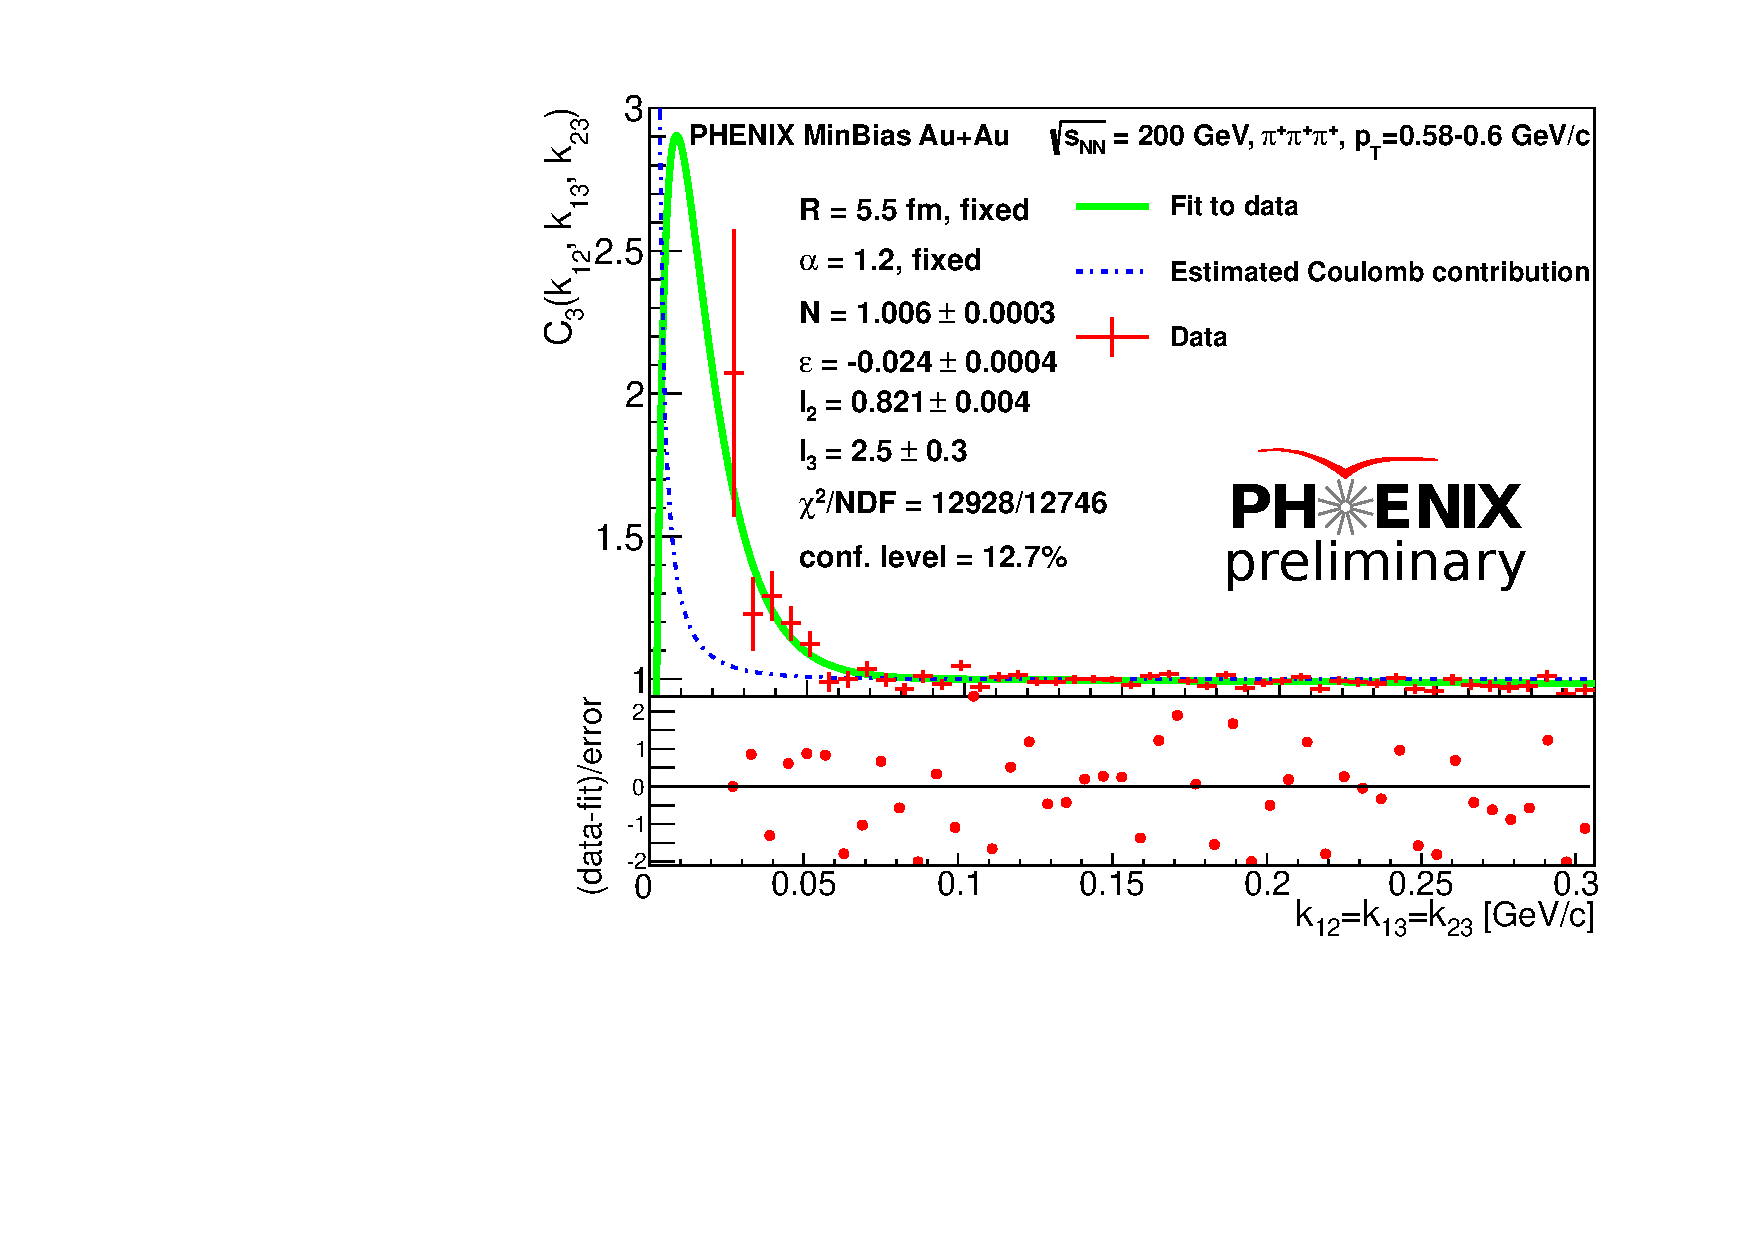
\includegraphics[scale=0.6]{pic/res/diag_highpt.pdf}
\caption{A háromrészecske korrelációs függvény illesztésének vizualizációja a $k_{12}=k_{23}=k_{31}$ altéren.}
\label{fig:fit}
\end{figure}



\subsection{Szisztematikus hibák}

Az előző fejezetekben láttuk, hogy a detektorok esetén különböző matching illetve párvágásokat alkalmazhatunk, amelyek a szisztematikus hiba leglényegesebb forrásai. A detektorrendszerből származó szisztematikus hiba mellett az illesztésnél előredefiniált paraméterek választása is hozzájárul a szisztematikus hibához (ezek közül az egyetlen jelentős hibaforrás az illesztési tartomány megválasztása). A szisztematikus hibaforrásokat és az alkalmazott vágásokat a következő lista foglalja össze:

\begin{itemize}
\item PID vágás: 3 különböző vágás ($1.5\sigma,\;2\sigma$ és $2.5\sigma$)
\item PC3 matching vágás: 3 különböző vágás ($1.5\sigma,\;2\sigma$ és $2.5\sigma$)
\item Matching vágás a PID detektorokban: 3 különböző vágás ($1.5\sigma,\;2\sigma$ és $2.5\sigma$)
\item Párvágás a DCH detektorban: három különböző vágás (\aref{tab:paircuts} táblázat 0,1,2 sora)
\item Párvágás a PID detektorban: három különböző vágás (\aref{tab:paircuts} táblázat 0,3,4 sora)
\item PID nyugati/keleti kar választása: három vágás (mindkető, keleti, nyugati)
\item Illesztés határának változtatása: $k_{\rm min}$ vágás (több vágás a $5-15$ MeV tartományban)
\end{itemize}

A szisztematikus hiba kiszámolása érdekében jelöljük az analízis során kapott mennyiségeket $P$-vel ($\lambda_3$, $\kappa_3$, $R$, $\alpha$). Az alapvágásoknál ennek az értékét jelöljük $P^0(i)$-val (ahol az $i$ az $m_T$ bin száma). Más vágások alkalmazása esetén a paraméter értéke megváltozhat, $n$ típusú vágás vizsgálata során a $j$-ik beállítás esetén a paraméter értékét jelöljük $P_n^j(i)$-vel. Adott $m_T$ esetén a $P$ paraméter szisztematikus hibáját a felső és alsó eltéréseket különválasztva a következőképpen számolhatjuk:

\begin{align}
\delta P^\uparrow(i)  &=\sqrt{\sum_{n={\rm cuts}}\frac{1}{N_n^{j\uparrow  }}\sum_{j\in J_n^\uparrow  }(P_n^j(i)-P^0(i))^2}\\
\delta P^\downarrow(i)&=\sqrt{\sum_{n={\rm cuts}}\frac{1}{N_n^{j\downarrow}}\sum_{j\in J_n^\downarrow}(P_n^j(i)-P^0(i))^2},
\end{align}
ahol $J_n^\uparrow$ azon $j$ értékek halmaza, amelyekre $P_n^j(i)>P^0(i)$, és $N_n^{j\uparrow}$ ezen halmaz számossága. Hasonlóan $J_n^\downarrow$ azon $j$ értékek halmaza amelyekre $P_n^j(i)<P^0(i)$, és  $N_n^{j\downarrow}$ ezen halmaz számossága. Az így kapott $\delta
P^\uparrow(i)$ és $\delta P^\downarrow(i)$ hibák nem fizikai fluktuációkat tartalmaznak, amelyeket egy $5$ pontos súlyozott átlagolással simítottunk ki.




\section{Eredmények}

Az analízis során a $\pi^-\pi^-\pi^-$ és $\pi^+\pi^+\pi^+$ triplettek közti Bose-Einstein korrelációt vizsgáltam. ~\Aref{sec:fit} fejezetben bemutatott $C_{3, \mathrm{fit}}^{(0)}$ modellt a Coulomb korrekciós integrállal osztva illesztettem a mérési adatokra, meghatározva a modell $R, \alpha, \ell_2, \ell_3, \varepsilon, N$ paramétereit. Az illesztéseket $m_T$ transzverz tömeg $32$ binjében végeztem, a $180-850$ MeV tartományban.

\subsection{Lévy eloszlás paraméterei}

A Lévy eloszlás $\alpha$ és $R$ sugárparaméterére a várakozásunk az volt, hogy megegyezik a kétrészecske analízisből kapott eredménnyel, hisz ezek a paraméterek a forrásra jellemzőek, és nem lehetnek érzékenyek arra, hogy hány részecske közti korrelációt vizsgálunk.  A várakozásunknak megfelelően az illesztésből kapott $R$ és $\alpha$ paraméter megegyezett a kétrészecske analízis során kapott paraméterekkel. Az utóbbiakat mutatja ~\aref{fig:aR} ábra. Az $\alpha(m_T)$ ábra mutatja, hogy ez a paraméter minden $m_T$ esetén jelentősen eltér az $\alpha=2$ esettől, azaz a Gauss eloszlástól.

Mivel a tesztillesztések során az $R$ és $\alpha$ paraméter megegyezett a kétrészecske analízisben meghatározott paraméterekkel, ezért a végső illesztésekben ezeket a paramétereket a lefixáltuk a kétrészecske analízisben kapott értékere (ezeket mutatja ~\aref{fig:aR} ábra). Ezzel az illesztési paraméterek számát $6$-ról $4$-re csökkentettük, ami jelentősen növelte az illesztési sebességet, valamint az illesztések stabilitását.

\begin{figure}[H]
\centering
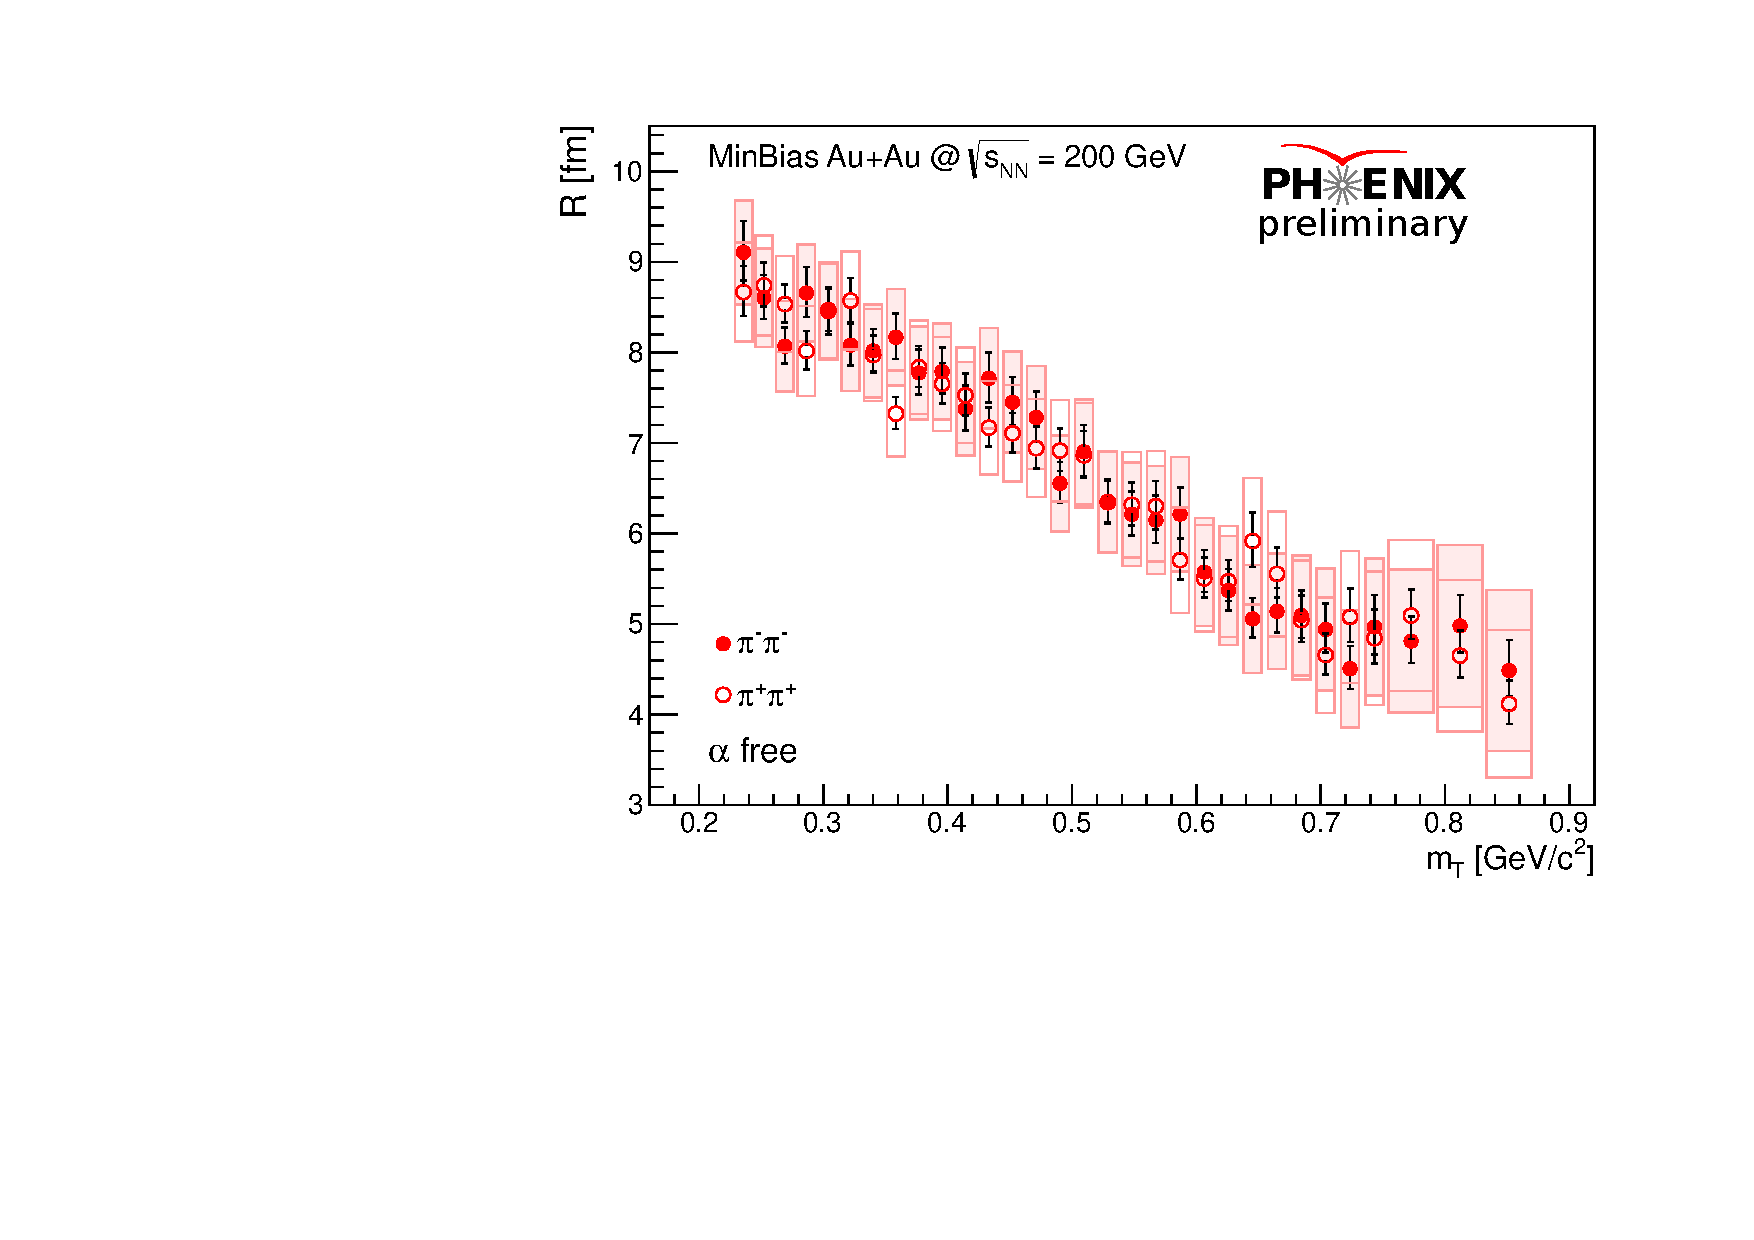
\includegraphics[scale=0.39]{pic/res/R_preliminary_stamp.pdf}
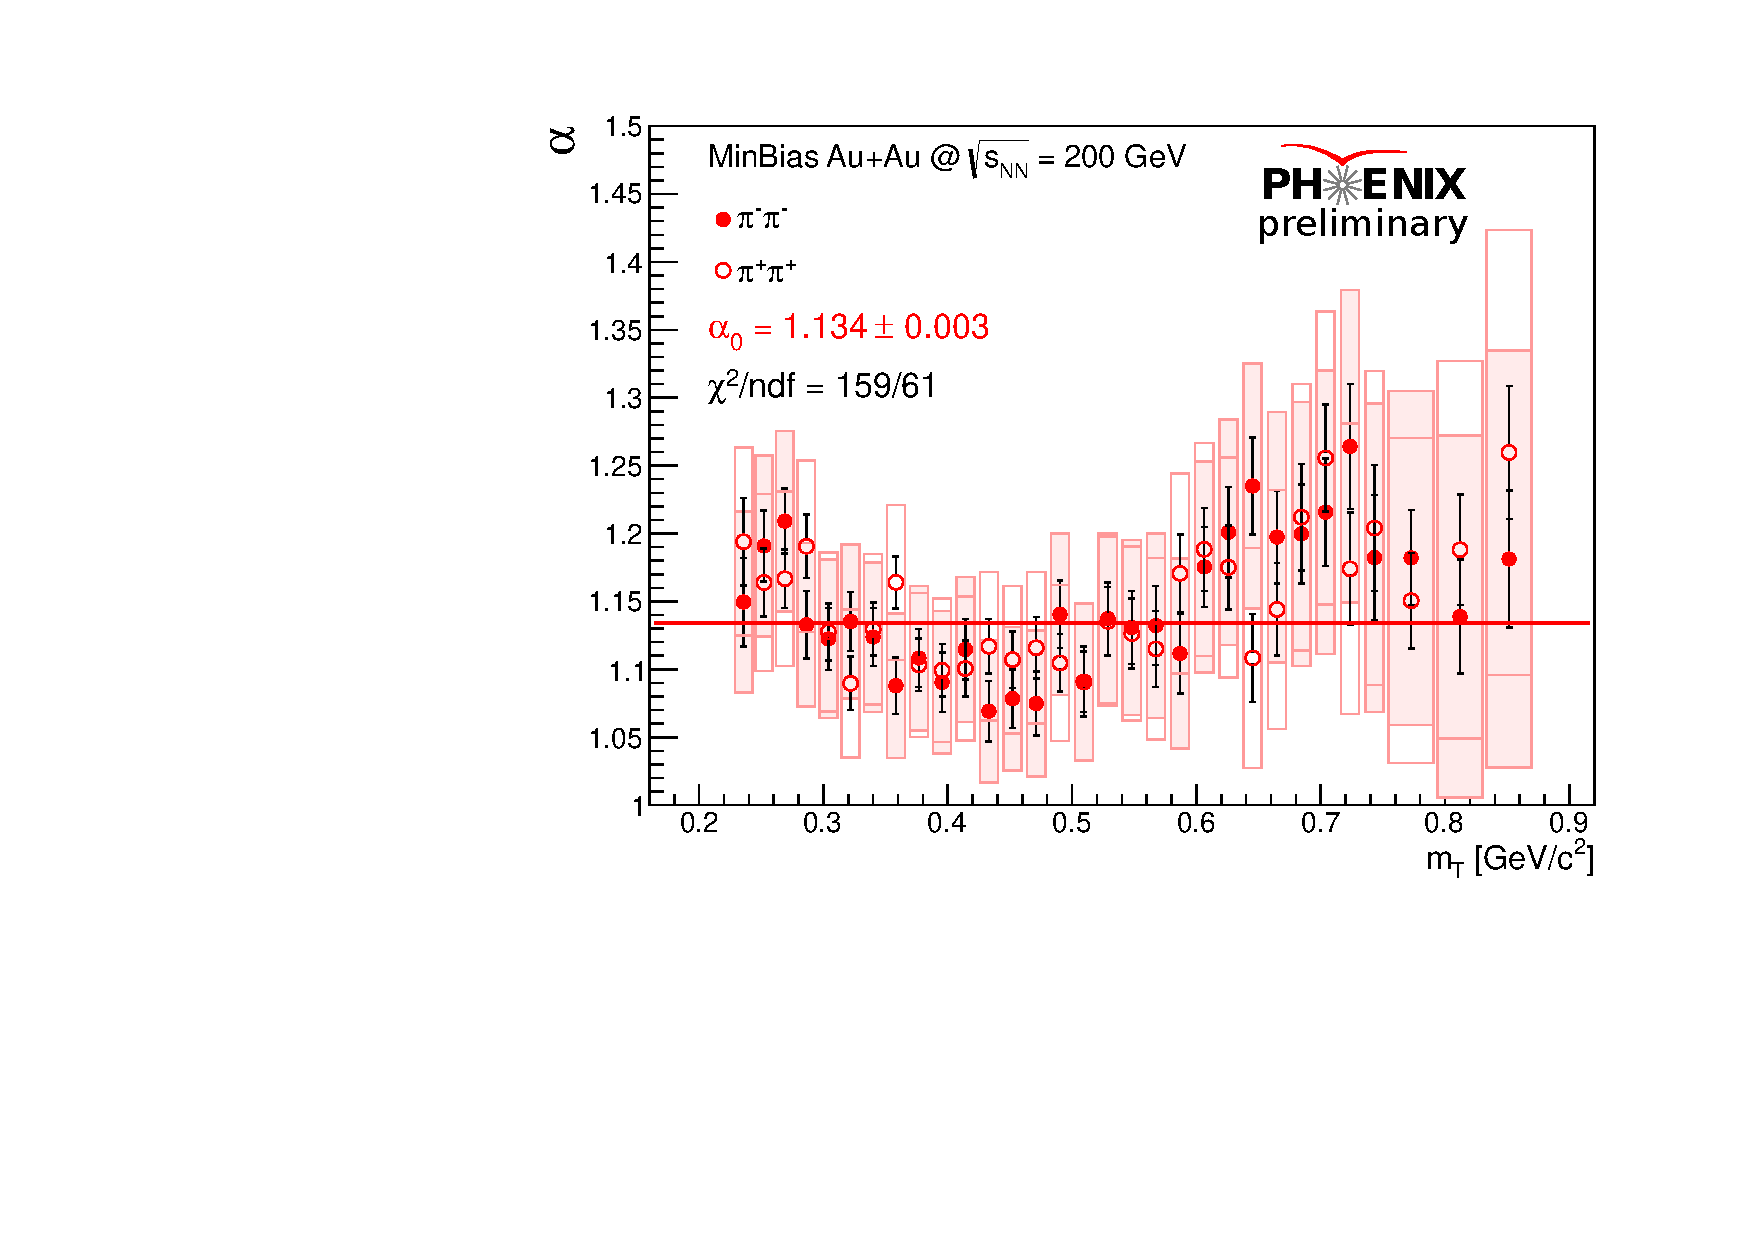
\includegraphics[scale=0.39]{pic/res/alpha_preliminary_stamp.pdf}
\caption{A kétrészecske analízis ~\cite{AN1244} során kapott $R$ és $\alpha$ illesztési paraméterek az $m_T$ függvényében.}
\label{fig:aR}
\end{figure}

\subsection{Háromrészecske korrelációs erősség}

Az $\ell_2$ és $\ell_3$ illesztési paraméterek segítségével a háromrészecske korreláció erősség megkapható: $\lambda_3=\ell_3-3\ell_2$. A korreláció erősségre kapott $m_T$ függést ~\aref{fig:lambda3} ábra mutatja. Az ábrán látható mag-glória modellben kaotikus forrás esetén a $\lambda_3$ megengedett tartománya (zöld doboz). Továbbá az ábrán kék dobozok mutatják a szisztematikus hibát, a szokásos hibajelzők pedig a statisztikus hibát. Az ábra mutatja, hogy a korrelációs erősség minden $m_T$ esetén a megengedett tartományban helyezkedik el.

\begin{figure}[H]
\centering
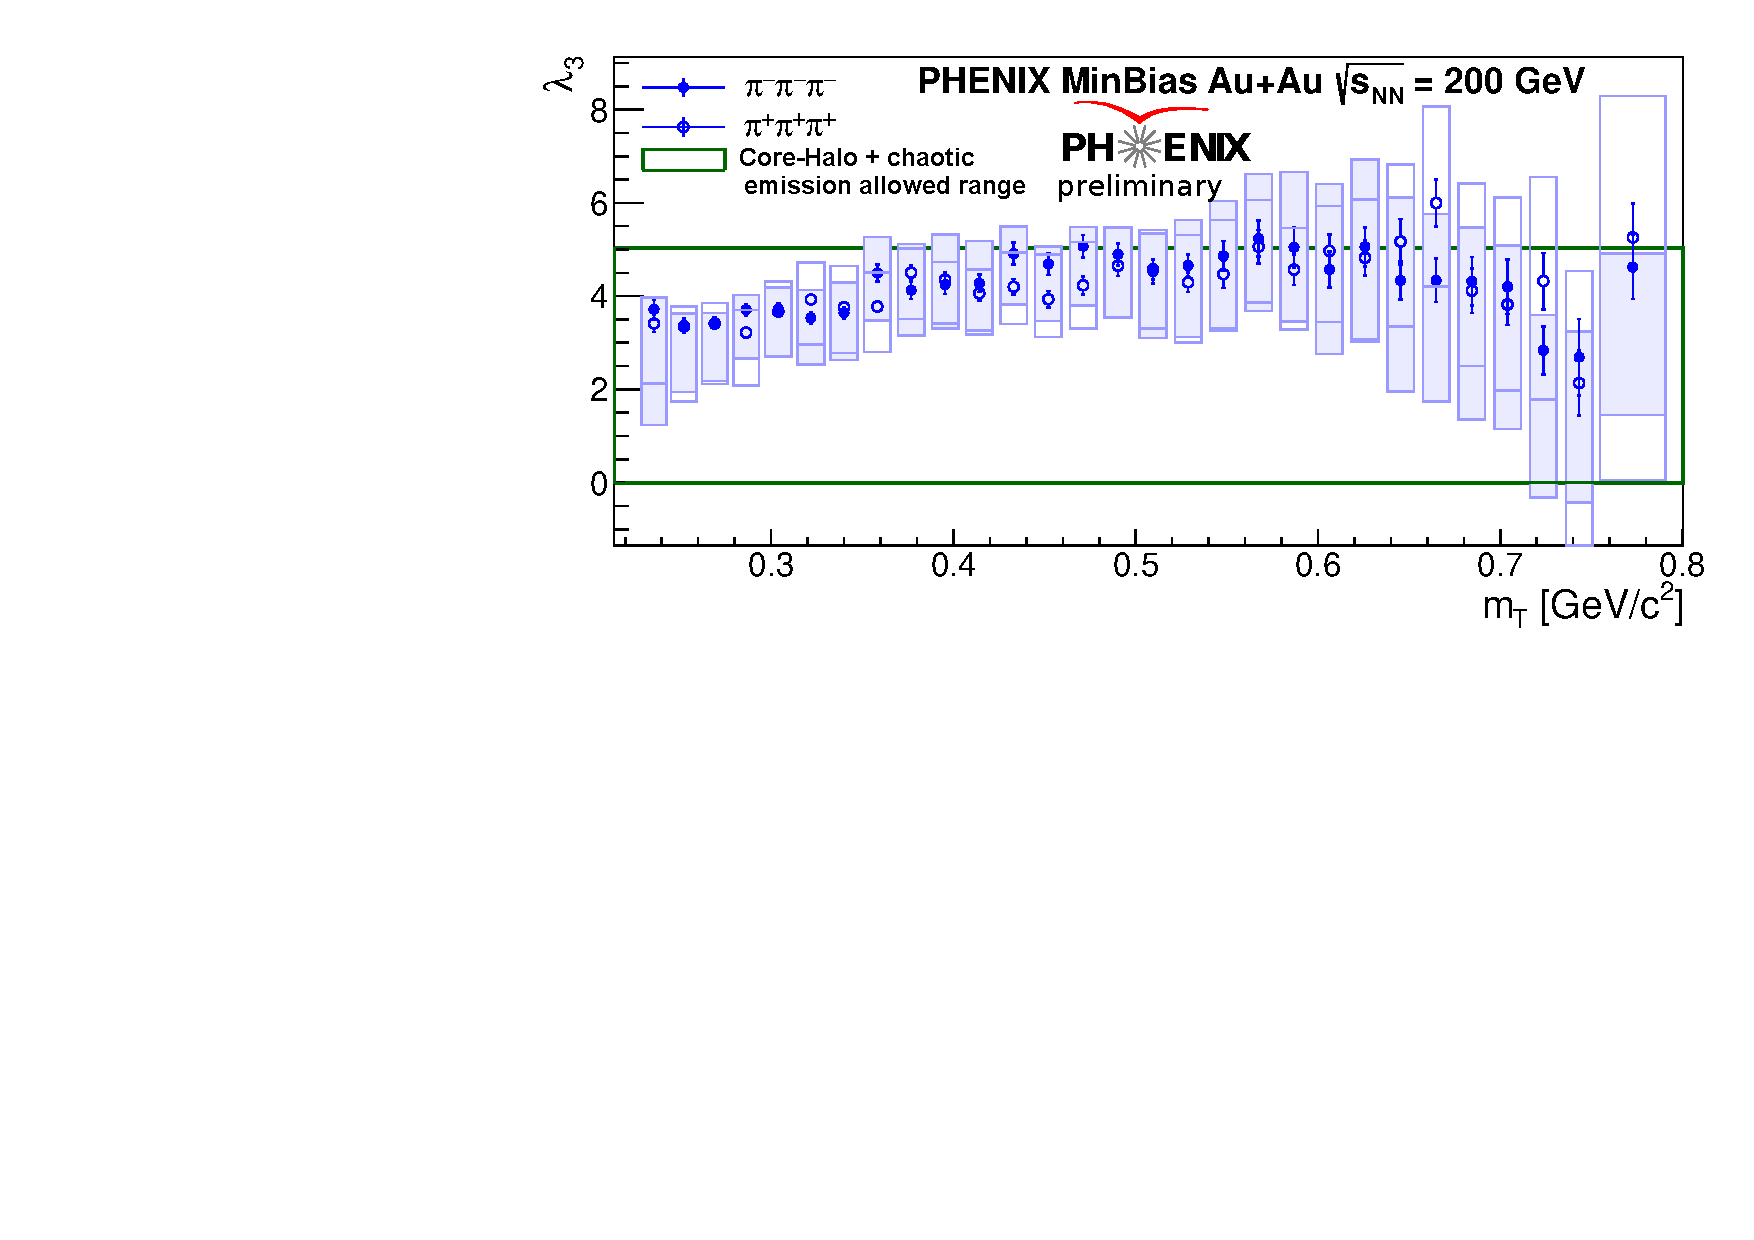
\includegraphics[scale=0.75]{pic/res/lambda3.pdf}
\caption{A háromrészecske korrelációs erősségének az $m_T$ függése. Az ábrán a pontok köré rajzolt dobozok mutatják a szisztematikus hibát.}
\label{fig:lambda3}
\end{figure}

\subsection{Parciális koherencia}

A mag-glória modell esetén már bevezettük a magarány paraméterét, valamint a parciális koherencia vizsgálata érdekében a koherensen keltett pionok arányát, melyeknek a definíciója az alábbi:
\begin{equation}
f_C=\frac{N_M}{N_M+N_G},\;\;\;\;\;\;\;\;\;\;\;p_C = \frac{N_M^C}{N_M^C+N_M^I},
\end{equation}
ahol $N_M$ a magban, $N_G$ a glóriában keletkezett részecskék száma. Az $N_M^C$ a magban koherensen keletkezett, $N_M^I$ az inkoherens módon keletkezett részecskék száma.

A két- és háromrészecske korrelációs erősségeknek ($\lambda_2,\;\lambda_3$) a már bevezetett, $\kappa_3$-al jelölt, kombinációjának specialitása, hogy nem függ az $f_C$ paramétertől, azaz tisztán mag-glória modell esetén $\kappa_3=1$ minden $m_T$-re. A paraméter a $\lambda_3,\; \lambda_2$ korrelációs erősségek alábbi kombinációja:

\begin{equation}
\kappa_3 = \frac{\lambda_3-3\lambda_2}{2\sqrt{\lambda_2^3}}
\end{equation}

Láttuk továbbá, hogy amennyiben a mag részben koherens módon kelt részecskéket, amit a $p_C$ paraméterrel jellemzünk, a $\kappa_3$ már nem lesz konstans, ehelyett valamilyen nem triviális $p_C$ függéssel rendelkezik. Azaz ha az $m_T$ függvényében a $p_C$ változik, akkor a $\kappa_3$ paraméter is fog változni az $m_T$ függvényében. ~\Aref{fig:kappa3} ábra mutatja ezen paraméter $m_T$ függését. Az ábra azt mutatja, hogy a $\kappa_3=1$ esettől statisztikailag szignifikáns eltérés van, amely lehetőség ad a parciális koherencia létezésére.

\begin{figure}[H]
\centering
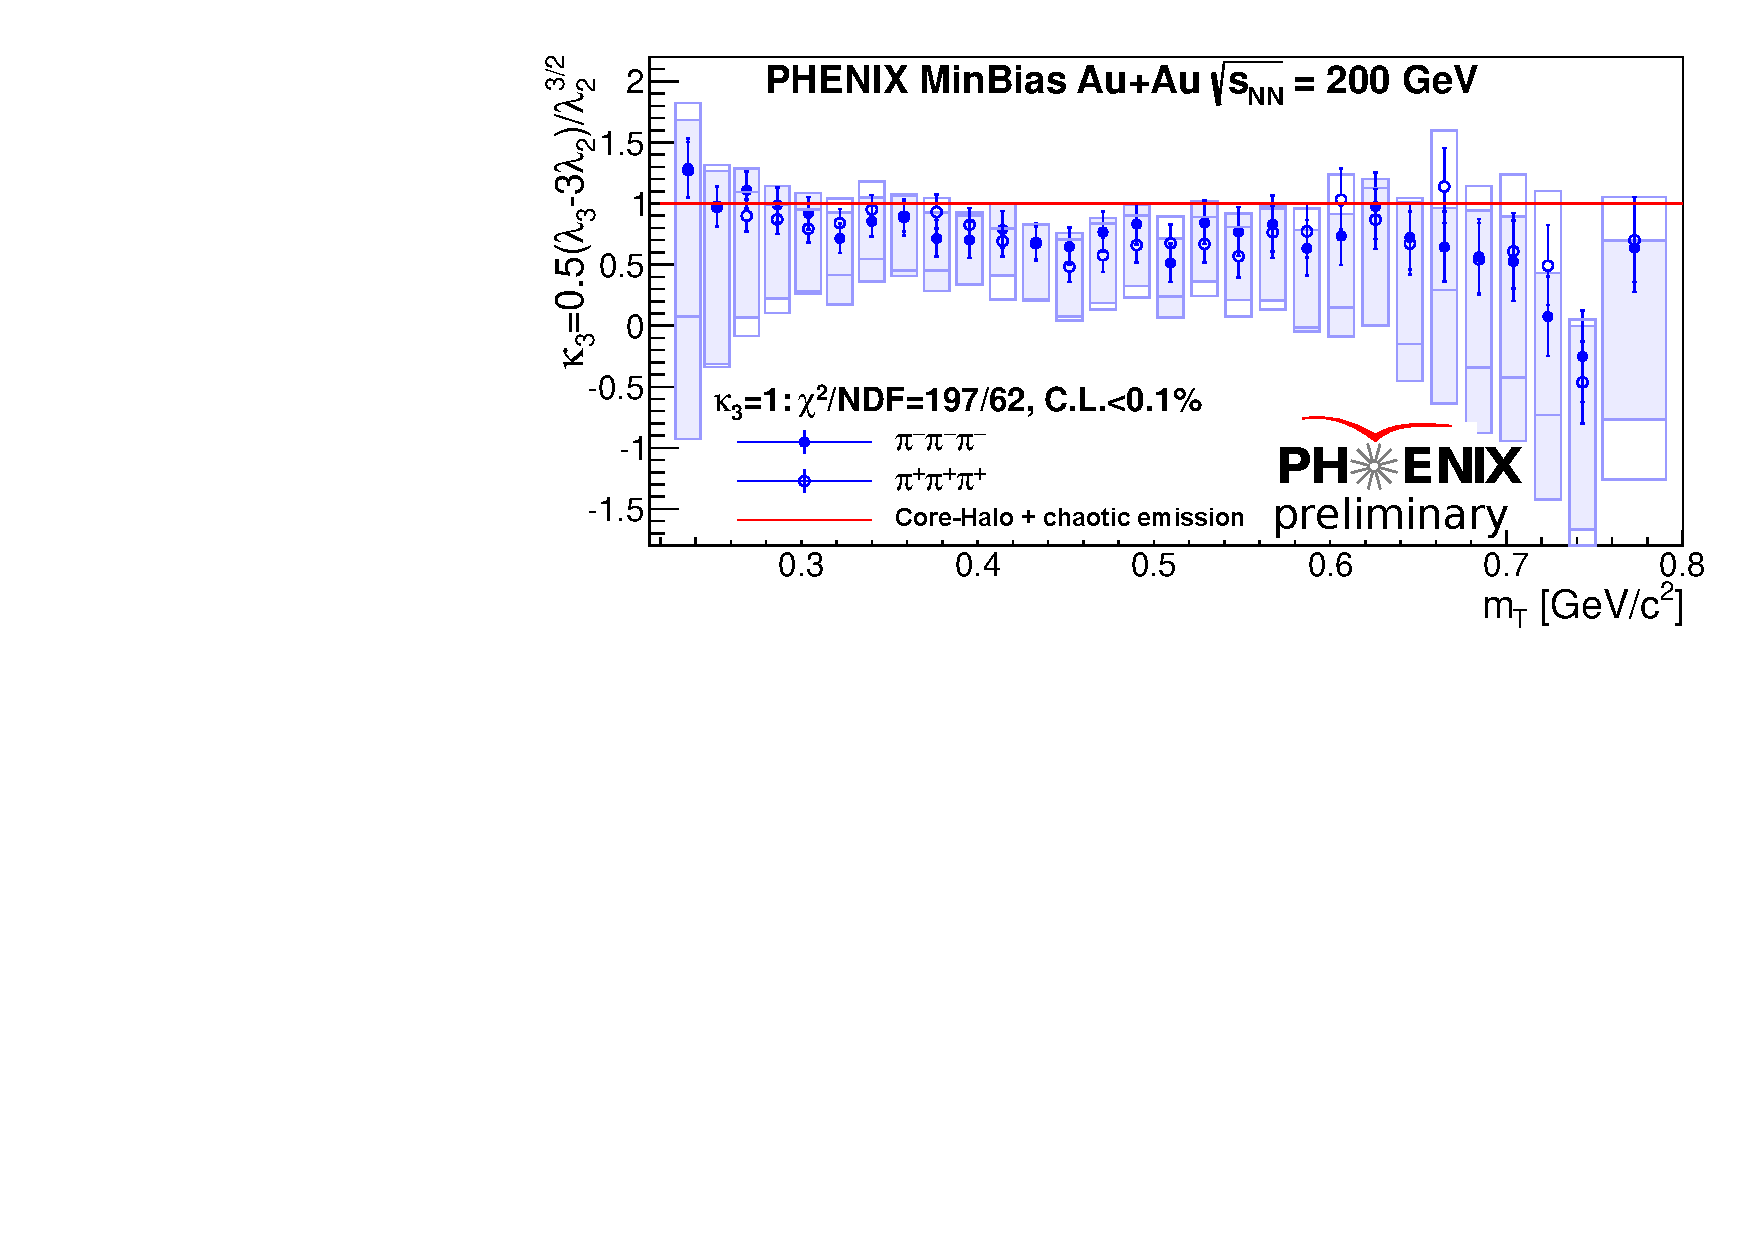
\includegraphics[scale=0.75]{pic/res/kappa3.pdf}
\caption{A $\kappa_3$ paraméter $m_T$ függése. Az ábrán a pontok köré rajzolt dobozok mutatják a szisztematikus hibát.}
\label{fig:kappa3}
\end{figure}

Mivel a $\kappa_3(m_T)$ ábra nem zárta ki a parciális koherencia létét, tovább vizsgáltuk ezt a jelenséget. Az előző fejezetekben tárgyaltam, hogy amennyiben létezik a jelenség, a két- és háromrészecske korrelációs erősségek a következő alakban írhatók fel:

\begin{equation}
\begin{aligned}
\lambda_2(f_C, p_C) =  f_C^2\big[(1-p_C)^2+2p_C(1-p_C)\big]\\
\lambda_3(f_C, p_C) =  2f_C^3\big[(1-p_C)^3+3p_C(1-p_C)^2\big]+3f_C^2\big[(1-p_C)^2+2p_C(1-p_C)\big]
\end{aligned}
\label{eq:l2l3}
\end{equation}

Adott $m_T$ esetén ismerjük a $\lambda_2$ és $\lambda_3$ korrelációs erősségeket. Ezeket ~\aref{eq:l2l3} összefüggésekbe beírva kapunk két egyenletet az $f_C$ paraméterre, mint a $p_C$ függvénye. Ezután a $0<p_C<1$ értékeire mindkét $f_C(p_C)$ függvényt ábrázolhatjuk. Ezt láthatjuk két különböző $m_T$ esetén ~\aref{fig:fcpc} ábrákon. Az ábrán a sávok mutatják az $1\sigma$ statisztikus hibát, amely a $\lambda_2,\;\lambda_3$ statisztikus hibájából adódik.

~\Aref{fig:fcpc} ábrák alapján a két vizsgált $m_T$ érték esetén kizárható a $80\%$-nál kisebb magarány. Kizárható továbbá a domináns parciális koherencia léte, azaz az $50\%$-nál több koherens módon keltett pion, a két vizsgált transzverz tömeg esetén. Azonban ezen ábrák alapján lehetséges az $50\%$-nál kisebb parciális koherencia. Sőt, az ábrák mutatják, hogy lehetőség van a koherencia arányának modellfüggő meghatározására. A koherencia aránya $\lambda_2$ és $\lambda_3$ görbék metszéspontjából kapható meg. Az ábrák alapján $m_T=250$ MeV esetén $p_C\approx 15\%$, $m_T=360$ MeV esetén pedig $p_C\approx 32\%$.

\begin{figure}[H]
\centering
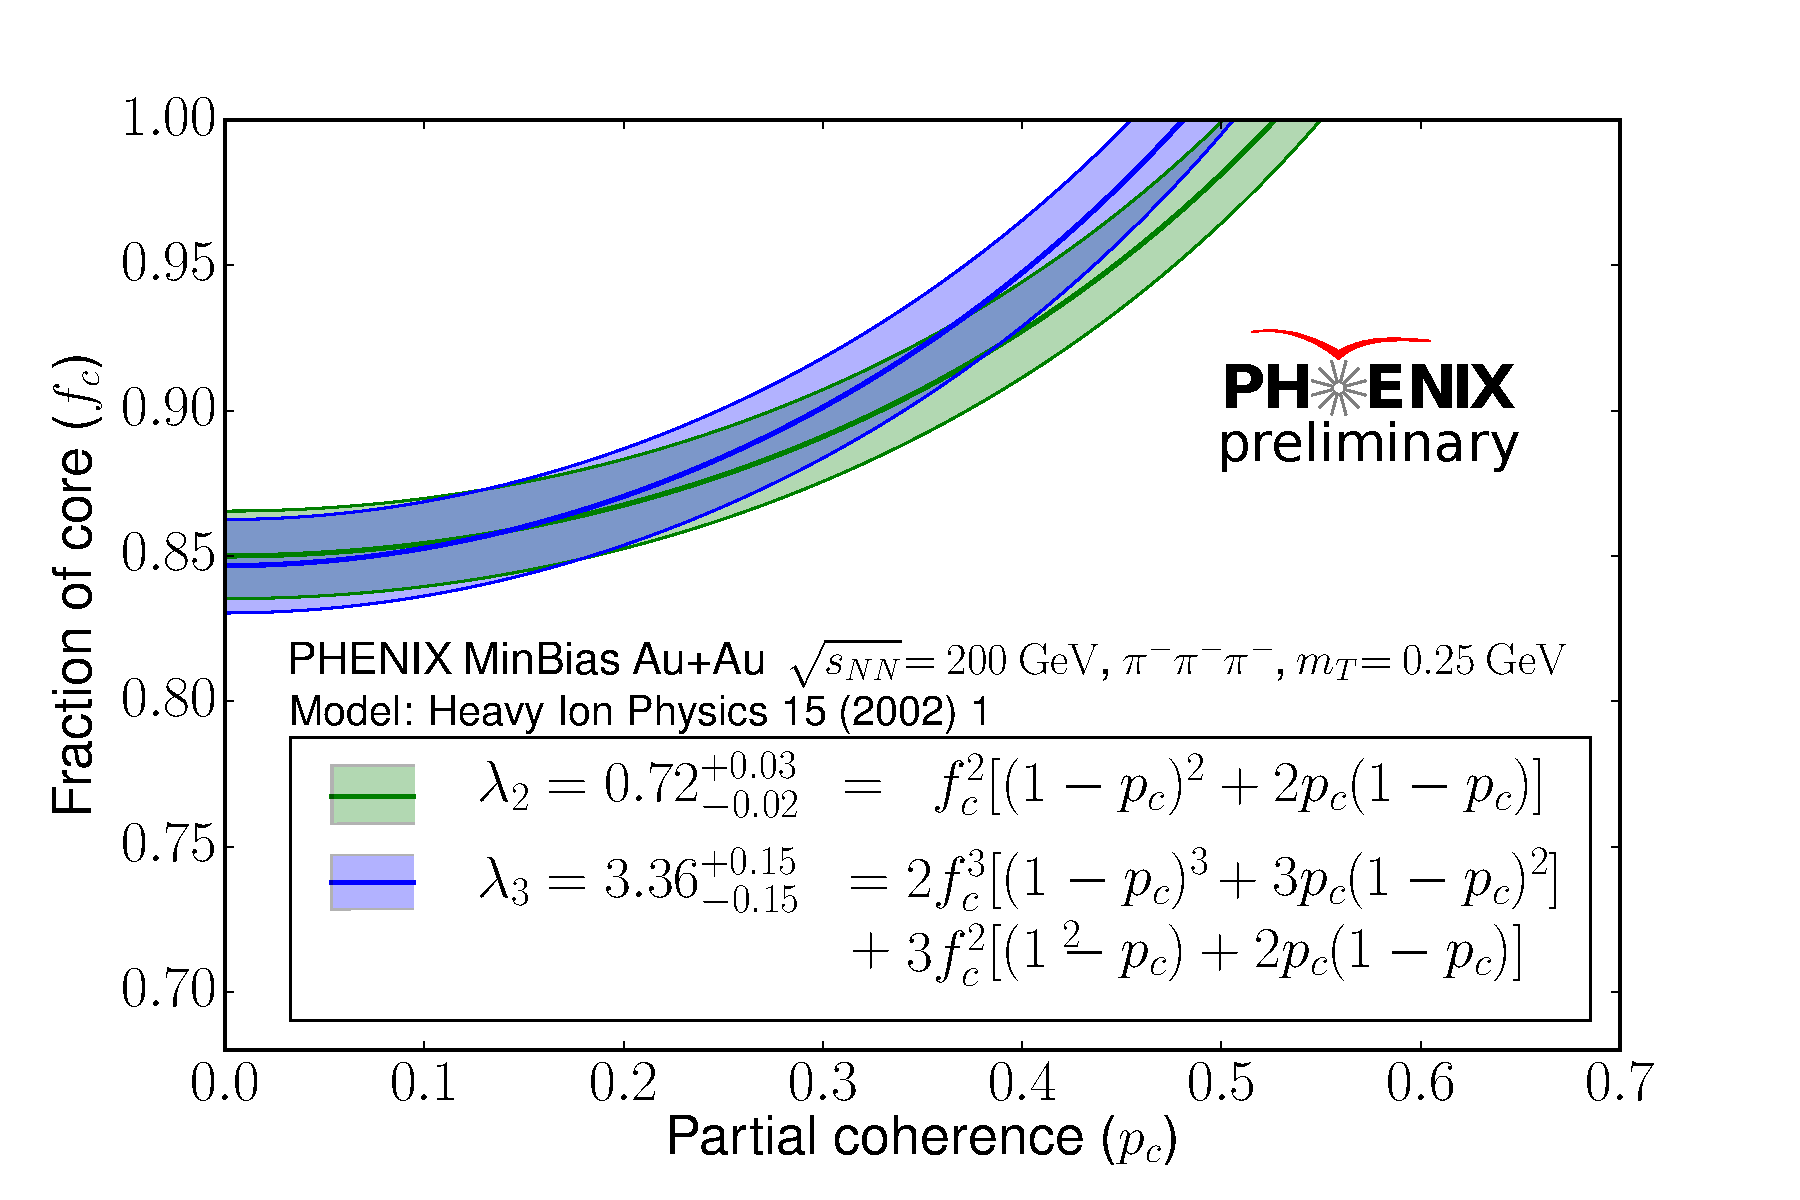
\includegraphics[scale=0.5]{pic/res/fcpc1.pdf}
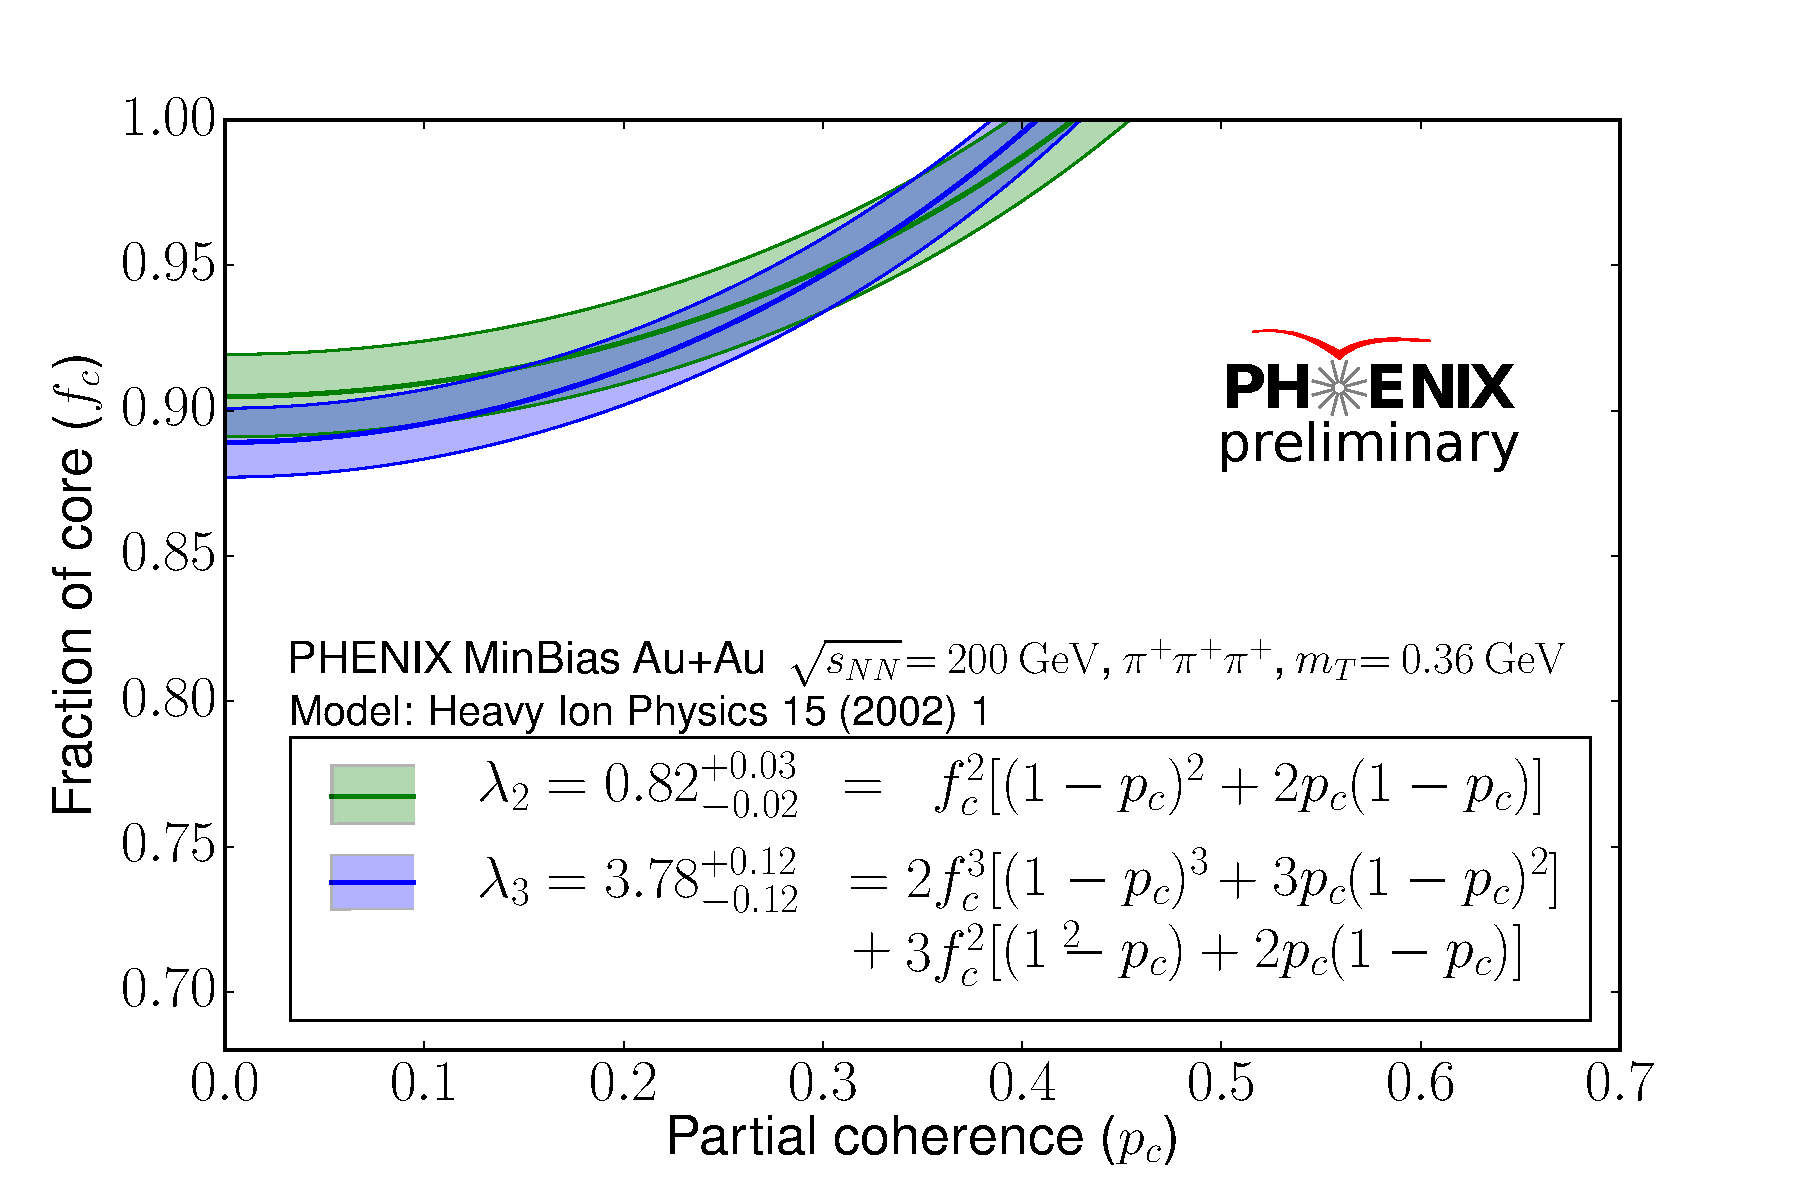
\includegraphics[scale=0.5]{pic/res/fcpc2.pdf}
\caption{A megmért $\lambda_2,\;\lambda_3$ paramétereket ~\aref{eq:l2l3} egyenletekbe helyesítve adódik a két $f_C(p_C)$ függvény. Az ábrán a sávok mutatják az $1\sigma$ statisztikai hibát.}
\label{fig:fcpc}
\end{figure}

\section{Összefoglaló}




\bibliography{ref}

\end{document}
